% arara: makeindex

% Template for IEEE papers
%% bare_conf.tex
%% V1.4b
%% 2015/08/26
%% by Michael Shell
%% See:
%% http://www.michaelshell.org/
%% for current contact information.
%%
%% This is a skeleton file demonstrating the use of IEEEtran.cls
%% (requires IEEEtran.cls version 1.8b or later) with an IEEE
%% conference paper.
%%
%% Support sites:
%% http://www.michaelshell.org/tex/ieeetran/
%% http://www.ctan.org/pkg/ieeetran
%% and
%% http://www.ieee.org/

%%*************************************************************************
%% Legal Notice:
%% This code is offered as-is without any warranty either expressed or
%% implied; without even the implied warranty of MERCHANTABILITY or
%% FITNESS FOR A PARTICULAR PURPOSE!
%% User assumes all risk.
%% In no event shall the IEEE or any contributor to this code be liable for
%% any damages or losses, including, but not limited to, incidental,
%% consequential, or any other damages, resulting from the use or misuse
%% of any information contained here.
%%
%% All comments are the opinions of their respective authors and are not
%% necessarily endorsed by the IEEE.
%%
%% This work is distributed under the LaTeX Project Public License (LPPL)
%% ( http://www.latex-project.org/ ) version 1.3, and may be freely used,
%% distributed and modified. A copy of the LPPL, version 1.3, is included
%% in the base LaTeX documentation of all distributions of LaTeX released
%% 2003/12/01 or later.
%% Retain all contribution notices and credits.
%% ** Modified files should be clearly indicated as such, including  **
%% ** renaming them and changing author support contact information. **
%%*************************************************************************


% *** Authors should verify (and, if needed, correct) their LaTeX system  ***
% *** with the testflow diagnostic prior to trusting their LaTeX platform ***
% *** with production work. The IEEE's font choices and paper sizes can   ***
% *** trigger bugs that do not appear when using other class files.       ***                          ***
% The testflow support page is at:
% http://www.michaelshell.org/tex/testflow/

\documentclass{book}
\usepackage[quiet]{fontspec}
\usepackage[table,xcdraw,dvipsnames]{xcolor} % Used by spritegrid and others.
\usepackage[obeyspaces,spaces]{url}
\usepackage{longtable}
\usepackage{arydshln}
\usepackage{booktabs}
\usepackage{afterpage}
\usepackage{flushend}
\usepackage{titletoc}
\usepackage[toc]{appendix}
\usepackage{parskip}
\usepackage{graphicx,wrapfig}
\usepackage{float}
\usepackage{caption}
\usepackage{pdfpages}
\usepackage{tikzpagenodes}
\usepackage{imakeidx}
\usepackage[pagestyles,raggedright]{titlesec}
\usepackage[all]{nowidow}
\usepackage[bookmarks=true]{hyperref}
\usepackage{aeb-minitoc}
\usepackage{fix-cm}
\usepackage{textpos}
\usepackage{enumitem}
\usepackage{tcolorbox}
\tcbuselibrary{listings}
%\usepackage{wrapfig}
\usepackage{needspace}
\usepackage{verbatim}
\usepackage{ean13isbn}
\usepackage{setspace}

% Use CHAPTER-PAGE page numbering to make it easier to modify chapters
% later, without messing up page number of the rest of the book.
\usepackage[auto]{chappg}

% Allow cross-references between the various books to the big The MEGA65 Book
\usepackage{xr}
\usepackage{varioref}
\usepackage{xparse}
\externaldocument[M65Book-]{mega65-book}
% And a \ref alternative that checks if it needs to be a cross-reference to the
% MEGA65 Book instead.
\makeatletter
\newcommand{\bookref}[1]{%
    \@ifundefined{r@#1}{%
      {\em the MEGA65 Book}, \nameref{M65Book-#1} (\autoref{M65Book-#1})}{\autoref{#1}}%
}
\newcommand{\bookvref}[1]{%
    \@ifundefined{r@#1}{%
      {\em the MEGA65 Book}, \nameref{M65Book-#1} (\autoref{M65Book-#1})}{Chapter/Appendix \vref{#1}}%
}
\makeatother

% For fixed-width columns in register maps
\usepackage{array}

% Makes tables with double-ruled lines look better
\usepackage{hhline}

% Makes better use of space for reference tables in appendix
\usepackage{multicol}

% Shaded tables with alternate rows colored for better legibility
% Best used with larger tables rather than small tables
\usepackage{colortbl}
\usepackage{adjustbox}
\usepackage[strict]{changepage}

% \makecell command for forcing line breaks in table cells
\usepackage{makecell}

\newcolumntype{L}[1]{>{\raggedright\let\newline\\\arraybackslash\hspace{0pt}}m{#1}}
\newcolumntype{C}[1]{>{\centering\let\newline\\\arraybackslash\hspace{0pt}}m{#1}}
\newcolumntype{R}[1]{>{\raggedleft\let\newline\\\arraybackslash\hspace{0pt}}m{#1}}

% For displaying Letter keys and the MEGA key
% This is a `keys' element for displaying a Mega65 keyboard key
% using a black filled label with rounded edges.
% In order to display a key as a title, use:
%
%     \megakey[title]{Run/Stop}
%
% For displaying a key as a part of the normal document flow, simply use:
%
%    \megakey{Shift}
%
%
% If you get warnings on special characters, mathematical characters etc, use $, eg:
%
%    \megakey{$\leftarrow$}
%
% Other sizes are supported, as part of tcolorbox:
% http://mirror.aarnet.edu.au/pub/CTAN/macros/latex/contrib/tcolorbox/tcolorbox.pdf#subsubsection.4.7.5 however, only `title' and the default: `small' are proposed for use in this manual.
%
% The second macro available here is the megasymbolkey.
% This will display the MEGA symbol as white on a black key box. Simply use:
%
%		 \megasymbolkey
%

\usepackage{tcolorbox}

\newtcbox{\megakeyinner}[1][small]{colback=black, coltext=white, size=#1, fontupper=\bfseries, nobeforeafter,box align=bottom,baseline=3pt,text height=7pt}
\newcommand{\megakey}[2][small]{\megakeyinner[#1]{\uppercase{#2}}}

\newtcbox{\megasymbolkeyinner}{colback=black, coltext=white, clip title=false. fontupper=\symbolfont, box align=bottom,baseline=3pt,text height=7pt}
\newcommand{\megasymbolkey}{\megakeyinner{\megasymbol[white]}\ }


% For displaying print versions petscii character symbols
% This is a collection of symbol macros element for displaying a printed version of the
% MEGA65 graphic characters, as opposed to the bitmap versions in the mega40/80.ttf fonts files.
% You can display characters using the graphicsymbol macro:
%
%    \graphicsymbol{\textcolor{red}{qQ} wWUcbdhjI \textcolor{blue}{JK}}
%
% Or you can, simply use the font itself:
%
%    \begin{symbolfont}%
%	   qQwWeErRtTyYuUiIoOpP\\
%		 aAsSdDfFgGhHjJkKlL\\
%		 zZxXcCvVbBnNmM%
%		 \end{symbolfont}%
%
%
% You can display the MEGA symbol using:
%
%    \megasymbol
%
% This will display the symbol in black. Other colours can be specified by passing them in, for example:
%
% 	 \megasymbol[black]
%		 \megasymbol[white]
%		 \megasymbol[orange]
%		 \megasymbol[blue]
%
% NOTE:
% For using the MEGA symbol in a key, see the \megasymbolkey macro in the keys.txt file.

\usepackage{tcolorbox}

\newcommand{\graphicsymbol}[1]{%
\begin{symbolfont}%
#1
\end{symbolfont}%
}%

\newcommand{\megasymbol}[1][black]{%
\begin{symbolfont}%
\textcolor{#1}{`}%
\end{symbolfont}%
\
}%


% For Mega65 display of code, listings and screen activity
% This is an element for displaying output from the Mega65 screen.
% It can display program code or to show activity on the screen.
% Example of use:
%
%    \begin{screenoutput}
%    10 OPEN 1,8,0,"$0:*,P,R
%    20 : IF DS THEN PRINT DS$: GOTO 100
%    30 GET#1,X$,X$
%    40 DO
%    50 : GET#1,X$,X$: IF ST THEN EXIT
%    60 : GET#1,BL$,BH$
%    70 : LINE INPUT#1, F$
%    80 : PRINT LEFT$(F$,18)
%    90 LOOP
%    100 CLOSE 1
%
%    RUN
%    \end{screenoutput}

\usepackage{listings,color}

\lstnewenvironment{screenoutput}
   {
     \lstset{
               basicstyle=\codefont\color{white}\linespread{1.1}\normalsize,
               backgroundcolor=\color{black},fillcolor=\color{black},
               frame=lines,
               rulecolor=\color{white},
               framexleftmargin=2mm,
               framexrightmargin=2mm,
               framextopmargin=2mm,
               framexbottommargin=2mm,
               tabsize=4,
               xleftmargin=2mm,
               xrightmargin=2mm,
               basewidth={0.4em},
               escapeinside={\%*}{*\%},
               literate={\*}{*}1{\-}{-}1{\/}{/}1{{\ }}{{ }}1
            }
   }
   {  }


% For in-line screen text
\newcommand{\screentext}[1]{ {\codefont\color{black}\normalsize{#1}} }



% For MEGA65 screen shots with text flow
\newcommand{\screenshotwrap}[1]{{\begin{center}\includegraphics[width=0.80\linewidth]{#1}\end{center}}}
%\newcommand{\screenshotwrap}[1]{\needspace{8cm}\setlength{\intextsep}{0pt}\begin{wrapfigure}{i}{0.80\textwidth}\includegraphics[width=\linewidth]{#1}\end{wrapfigure}}


% For displaying sprite data in a grid
% This is an element for displaying a sprite in a grid, just like page 70 of the
% commodore manual. This version can be easily expanded. For now it will suffice.
% In order to display a hi-res mono sprite grid use:
%
%	\spritegrid{
%	\hline
%	\spritecells{---------ooooo----------}
%	\spritecells{-------ooooooooo--------}
%	\spritecells{------ooooooooooo-------}
%	\spritecells{------ooo--o---oo-------}
%	\spritecells{-----ooo-ooo-ooooo------}
%	\spritecells{-----ooo-ooo-ooooo------}
%	\spritecells{-----ooo---o---ooo------}
%	\spritecells{-----ooo-o-ooo-ooo------}
%	\spritecells{-----ooo-o-ooo-ooo------}
%	\spritecells{-----ooo---o--oooo------}
%	\spritecells{------ooooooooooo-------}
%	\spritecells{------ooooooooooo-------}
%	\spritecells{-------ooooooooo--------}
%	\spritecells{-------o-ooooo-o--------}
%	\spritecells{--------o-o-o-o---------}
%	\spritecells{--------o--o--o---------}
%	\spritecells{---------o-o-o----------}
%	\spritecells{---------o-o-o----------}
%	\spritecells{---------ooooo----------}
%	\spritecells{---------ooooo----------}
%	\spritecells{----------ooo-----------}
%	}
%
% For a multicolour sprite:
%
%	\spritegrid{
%	\hline
%	\spritecells{------------------------}
%	\spritecells{------------------------}
%	\spritecells{------------------------}
%	\spritecells{------------------------}
%	\spritecells{--------llllll----------}
%	\spritecells{------llllllggll--------}
%	\spritecells{------llllllllgg--------}
%	\spritecells{----llllllgggggggg------}
%	\spritecells{----llllggeeeellll------}
%	\spritecells{----lloollllllggee------}
%	\spritecells{----llooggggooggee------}
%	\spritecells{----llooggggooggee------}
%	\spritecells{----eeeeggggooeeee------}
%	\spritecells{----ggeeeeeeeeoo--------}
%	\spritecells{------ggooooooee--------}
%	\spritecells{------eeggeeeeee--------}
%	\spritecells{--------eeeeee----------}
%	\spritecells{------------------------}
%	\spritecells{------------------------}
%	\spritecells{------------------------}
%	\spritecells{------------------------}
%	}

\usepackage{tabulary} %Removes spacing from tabulars
\usepackage{xstring} % for string substitution
\usepackage{xparse} % used for unpacking the sprite characters
% \renewcommand{\familydefault}{\sfdefault} % default sans font

%\usepackage{graphicx} % for resizing the tabular used by spritegrid
\usepackage{subcaption} % used for the left hand subtable of row numbers
\usepackage{multirow} % used for the ``Row'' column
\usepackage{rotating} % used by the rotating ``Row'' word

\newcommand{\spritebytecolumn}[1]{
   %\framebox[4mm]{#1}
   \makebox[4mm]{#1}
}

\setlength\tabcolsep{0.3mm} % the indivdual cell width and height


% Cell colour list. Can be expanded for other colours in the sprite grid
\def\blk{\cellcolor{black}}
\def\wht{\cellcolor{white}}
\def\grn{\cellcolor{ForestGreen}}
\def\lgrn{\cellcolor{YellowGreen}}
\def\gry{\cellcolor{Gray}}

\newcounter{lettercounter} % counter for detecting the last cell

% Collect the spritecell list and send it to \ProcessSpriteCell for turning into cells
\NewDocumentCommand{\spritecells}{%
>{\SplitList{}} m }{%
  \ProcessList{#1}{\ProcessSpriteCell}%
}

\NewDocumentCommand{\ProcessSpriteCell}{m}{%
  \stepcounter{lettercounter}%
    \IfStrEqCase{#1}{
	{o}{\blk}
	{-}{\wht}
	{g}{\grn}
	{l}{\lgrn}
	{e}{\gry}
   }%
   \IfStrEq{\thelettercounter}{24}{\setcounter{lettercounter}{0} \\ \hline}{&}%
}

% Start of the actual spritegrid definition
\newcommand{\spritegrid}[1]{
\begin{table}[h!]
\centering
\begin{subtable}{28mm}
\vspace{8mm}
\scalebox{0.76}{
\begin{tabular}{p{25mm} p{4mm} c}
\multirow{21}{*}{ } &
\multirow{21}{*}{%
\begin{turn}{90}%
\bfseries\uppercase{Row}%
\end{turn}} &
 1\\
& & 2\\
& & 3\\
& & 4\\
& & 5\\
& & 6\\
& & 7\\
& & 8\\
& & 9\\
& & 10\\
& & 11\\
& & 12\\
& & 13\\
& & 14\\
& & 15\\
& & 16\\
& & 17\\
& & 18\\
& & 19\\
& & 20\\
& & 21
\end{tabular}
}
\end{subtable}%
\begin{subtable}{.8\textwidth}

\setlength{\arrayrulewidth}{1pt}
\scalebox{0.7}{
\begin{tabular}{  *{3}{p{30mm} }  }
  \center\uppercase{Series\\1} &
  \center\uppercase{Series\\2} &
  \center\uppercase{Series\\3}
\end{tabular}
}

\scalebox{0.7}{
\begin{tabular}{p{5.8mm} *{11}{C{7.3mm}}}
   128 & 32 & 8 & 2 & 128 & 32 & 8 & 2 & 128 & 32 & 8 & 2
\end{tabular}
}
\\[-1.5mm]
\scalebox{0.7}{
\begin{tabular}{p{1.7mm} *{12}{C{7.3mm}}}
  & 64 & 16 & 4 & 1 & 64 & 16 & 4 & 1 & 64 & 16 & 4 & 1
\end{tabular}
}

\scalebox{0.7}{
\begin{tabular}{ | *{24}{p{3mm} |}  }
#1
\end{tabular}
}

\scalebox{0.7}{
\begin{tabular}{ *{24}{p{3.35mm}}  }
	\spritebytecolumn{1} & & & &
	\spritebytecolumn{5} & & & & &
	\spritebytecolumn{10} & & & & &
	\spritebytecolumn{15} & & & & &
	\spritebytecolumn{20} & & & &
	\spritebytecolumn{24} \\
	\multicolumn{24}{c}{\bfseries\uppercase{Column}}
\end{tabular}
}
\end{subtable}
\end{table}
}

% End of the actual spritegrid definition



% Don't number sections
\setcounter{secnumdepth}{0}

\renewcommand{\indexname}{INDEX}
\renewcommand{\appendixtocname}{APPENDICES}
\renewcommand{\appendixpagename}{APPENDICES}
\renewcommand{\appendixpage}{%
  \clearpage\thispagestyle{empty}
    \pagecolor{blue}
     \begin{center}
       {
         \large
         % Put a nice amount of vertical space before the title
         \vspace*{2cm}
               {\large\Huge\textcolor{white}{\bf{APPENDICES}}}\\
             \vspace{\fill}
       }
     \end{center}
     \newpage\pagecolor{white}\clearpage
}

\makeatletter\chardef\pdf@shellescape=\@ne\makeatother

\setcounter{tocdepth}{5}

% 1.0 cm is the distance from left of page to bullet point.
% 2.8 cm is a fudge-factor to make multi-line section names be correctly lined up.
% \@B{〈length〉} is the amount to indent prior to〈sec-num >
% \@F{〈fmt〉} is the formatting for the title heading
% \@P{〈fmt〉} is the formatting for the page number (〈pg-num〉).

\TOCLevels{chapter}{section}
\begin{minitocfmt}{\chapmtoc}
\declaretocfmt{section}{\@F{\color{white}\hspace{1.0cm}\textbullet\hspace{0.25cm}\Large\bfseries}\@B{2.8cm}\@P{\mtocgobble}}
\declaretocfmt{section*}{\@F{\color{white}\hspace{1.0cm}\textbullet\hspace{0.25cm}\Large\bfseries}\@B{2.8cm}\@P{\mtocgobble}}
\end{minitocfmt}

\usepackage{fontspec}

\setmainfont[Path=fonts/, BoldFont=MegaGlacial-Bold.otf, ItalicFont=MegaGlacial-Italic.otf]{MegaGlacial-Regular.otf}
%\setmainfont[Path=fonts/, BoldFont=GlacialIndifference-Bold.otf, ItalicFont=GlacialIndifference-Italic.otf]{GlacialIndifference-Regular.otf}
\newfontfamily\serifed[Path=fonts/, BoldFont=xits-bold.otf, ItalicFont=xits-italic.otf]{xits-regular.otf}
\newfontface\codefont[Path=fonts/]{mega80.ttf}
\newfontface\symbolfont[Path=fonts/]{MEGA65GraphicSymbols.otf}


% Set margins for inner and outer pages in A5 book format
\ifdefined\printmanual
\usepackage[a5paper,nomarginpar,includemp,bottom=2cm,top=1cm,inner=1.8cm,outer=0.8cm, footskip = 1cm]{geometry}
\else
\usepackage[a5paper,nomarginpar,includemp,bottom=2cm,top=1cm,inner=1.0cm,outer=1.0cm, footskip = 1cm]{geometry}
\fi

% Some Computer Society conferences also require the compsoc mode option,
% but others use the standard conference format.
%
% If IEEEtran.cls has not been installed into the LaTeX system files,
% manually specify the path to it like:
% \documentclass[conference]{../sty/IEEEtran}

%% % Some very useful LaTeX packages include:

% *** MISC UTILITY PACKAGES ***
%
%\usepackage{ifpdf}
% Heiko Oberdiek's ifpdf.sty is very useful if you need conditional
% compilation based on whether the output is pdf or dvi.
% usage:
% \ifpdf
%   % pdf code
% \else
%   % dvi code
% \fi
% The latest version of ifpdf.sty can be obtained from:
% http://www.ctan.org/pkg/ifpdf
% Also, note that IEEEtran.cls V1.7 and later provides a builtin
% \ifCLASSINFOpdf conditional that works the same way.
% When switching from latex to pdflatex and vice-versa, the compiler may
% have to be run twice to clear warning/error messages.



\usepackage{csquotes}


% *** CITATION PACKAGES ***
%
\usepackage{cite}
% cite.sty was written by Donald Arseneau
% V1.6 and later of IEEEtran pre-defines the format of the cite.sty package
% \cite{} output to follow that of the IEEE. Loading the cite package will
% result in citation numbers being automatically sorted and properly
% "compressed/ranged". e.g., [1], [9], [2], [7], [5], [6] without using
% cite.sty will become [1], [2], [5]--[7], [9] using cite.sty. cite.sty's
% \cite will automatically add leading space, if needed. Use cite.sty's
% noadjust option (cite.sty V3.8 and later) if you want to turn this off
% such as if a citation ever needs to be enclosed in parenthesis.
% cite.sty is already installed on most LaTeX systems. Be sure and use
% version 5.0 (2009-03-20) and later if using hyperref.sty.
% The latest version can be obtained at:
% http://www.ctan.org/pkg/cite
% The documentation is contained in the cite.sty file itself.






% *** GRAPHICS RELATED PACKAGES ***
%
\ifCLASSINFOpdf
   \usepackage[pdftex]{graphicx}
  % declare the path(s) where your graphic files are
   \graphicspath{{../pdf/}{../jpeg/}}
  % and their extensions so you won't have to specify these with
  % every instance of \includegraphics
   \DeclareGraphicsExtensions{.pdf,.jpeg,.png}
\else
  % or other class option (dvipsone, dvipdf, if not using dvips). graphicx
  % will default to the driver specified in the system graphics.cfg if no
  % driver is specified.
   \usepackage[dvips]{graphicx}
  % declare the path(s) where your graphic files are
%   \graphicspath{{../eps/}}
  % and their extensions so you won't have to specify these with
  % every instance of \includegraphics
   \DeclareGraphicsExtensions{.eps}
\fi
% graphicx was written by David Carlisle and Sebastian Rahtz. It is
% required if you want graphics, photos, etc. graphicx.sty is already
% installed on most LaTeX systems. The latest version and documentation
% can be obtained at: 
% http://www.ctan.org/pkg/graphicx
% Another good source of documentation is "Using Imported Graphics in
% LaTeX2e" by Keith Reckdahl which can be found at:
% http://www.ctan.org/pkg/epslatex
%
% latex, and pdflatex in dvi mode, support graphics in encapsulated
% postscript (.eps) format. pdflatex in pdf mode supports graphics
% in .pdf, .jpeg, .png and .mps (metapost) formats. Users should ensure
% that all non-photo figures use a vector format (.eps, .pdf, .mps) and
% not a bitmapped formats (.jpeg, .png). The IEEE frowns on bitmapped formats
% which can result in "jaggedy"/blurry rendering of lines and letters as
% well as large increases in file sizes.
%
% You can find documentation about the pdfTeX application at:
% http://www.tug.org/applications/pdftex





% *** MATH PACKAGES ***
%
%\usepackage{amsmath}
% A popular package from the American Mathematical Society that provides
% many useful and powerful commands for dealing with mathematics.
%
% Note that the amsmath package sets \interdisplaylinepenalty to 10000
% thus preventing page breaks from occurring within multiline equations. Use:
%\interdisplaylinepenalty=2500
% after loading amsmath to restore such page breaks as IEEEtran.cls normally
% does. amsmath.sty is already installed on most LaTeX systems. The latest
% version and documentation can be obtained at:
% http://www.ctan.org/pkg/amsmath





% *** SPECIALIZED LIST PACKAGES ***
%
%\usepackage{algorithmic}
% algorithmic.sty was written by Peter Williams and Rogerio Brito.
% This package provides an algorithmic environment fo describing algorithms.
% You can use the algorithmic environment in-text or within a figure
% environment to provide for a floating algorithm. Do NOT use the algorithm
% floating environment provided by algorithm.sty (by the same authors) or
% algorithm2e.sty (by Christophe Fiorio) as the IEEE does not use dedicated
% algorithm float types and packages that provide these will not provide
% correct IEEE style captions. The latest version and documentation of
% algorithmic.sty can be obtained at:
% http://www.ctan.org/pkg/algorithms
% Also of interest may be the (relatively newer and more customizable)
% algorithmicx.sty package by Szasz Janos:
% http://www.ctan.org/pkg/algorithmicx




% *** ALIGNMENT PACKAGES ***
%
%\usepackage{array}
% Frank Mittelbach's and David Carlisle's array.sty patches and improves
% the standard LaTeX2e array and tabular environments to provide better
% appearance and additional user controls. As the default LaTeX2e table
% generation code is lacking to the point of almost being broken with
% respect to the quality of the end results, all users are strongly
% advised to use an enhanced (at the very least that provided by array.sty)
% set of table tools. array.sty is already installed on most systems. The
% latest version and documentation can be obtained at:
% http://www.ctan.org/pkg/array


% IEEEtran contains the IEEEeqnarray family of commands that can be used to
% generate multiline equations as well as matrices, tables, etc., of high
% quality.

%%%%%%%%%%%%%%%%%
\usepackage{multirow}
\usepackage[table]{xcolor}
\usepackage{tablefootnote}
\usepackage[bottom]{footmisc}

%%%%%%%%%%%%%%%%%%

% *** SUBFIGURE PACKAGES ***
\ifCLASSOPTIONcompsoc
  \usepackage[caption=false,font=normalsize,labelfont=sf,textfont=sf]{subfig}
\else
  \usepackage[caption=false,font=footnotesize]{subfig}
\fi
% subfig.sty, written by Steven Douglas Cochran, is the modern replacement
% for subfigure.sty, the latter of which is no longer maintained and is
% incompatible with some LaTeX packages including fixltx2e. However,
% subfig.sty requires and automatically loads Axel Sommerfeldt's caption.sty
% which will override IEEEtran.cls' handling of captions and this will result
% in non-IEEE style figure/table captions. To prevent this problem, be sure
% and invoke subfig.sty's "caption=false" package option (available since
% subfig.sty version 1.3, 2005/06/28) as this is will preserve IEEEtran.cls
% handling of captions.
% Note that the Computer Society format requires a larger sans serif font
% than the serif footnote size font used in traditional IEEE formatting
% and thus the need to invoke different subfig.sty package options depending
% on whether compsoc mode has been enabled.
%
% The latest version and documentation of subfig.sty can be obtained at:
% http://www.ctan.org/pkg/subfig




% *** FLOAT PACKAGES ***
%
%\usepackage{fixltx2e}
% fixltx2e, the successor to the earlier fix2col.sty, was written by
% Frank Mittelbach and David Carlisle. This package corrects a few problems
% in the LaTeX2e kernel, the most notable of which is that in current
% LaTeX2e releases, the ordering of single and double column floats is not
% guaranteed to be preserved. Thus, an unpatched LaTeX2e can allow a
% single column figure to be placed prior to an earlier double column
% figure.
% Be aware that LaTeX2e kernels dated 2015 and later have fixltx2e.sty's
% corrections already built into the system in which case a warning will
% be issued if an attempt is made to load fixltx2e.sty as it is no longer
% needed.
% The latest version and documentation can be found at:
% http://www.ctan.org/pkg/fixltx2e


%\usepackage{stfloats}
% stfloats.sty was written by Sigitas Tolusis. This package gives LaTeX2e
% the ability to do double column floats at the bottom of the page as well
% as the top. (e.g., "\begin{figure*}[!b]" is not normally possible in
% LaTeX2e). It also provides a command:
%\fnbelowfloat
% to enable the placement of footnotes below bottom floats (the standard
% LaTeX2e kernel puts them above bottom floats). This is an invasive package
% which rewrites many portions of the LaTeX2e float routines. It may not work
% with other packages that modify the LaTeX2e float routines. The latest
% version and documentation can be obtained at:
% http://www.ctan.org/pkg/stfloats
% Do not use the stfloats baselinefloat ability as the IEEE does not allow
% \baselineskip to stretch. Authors submitting work to the IEEE should note
% that the IEEE rarely uses double column equations and that authors should try
% to avoid such use. Do not be tempted to use the cuted.sty or midfloat.sty
% packages (also by Sigitas Tolusis) as the IEEE does not format its papers in
% such ways.
% Do not attempt to use stfloats with fixltx2e as they are incompatible.
% Instead, use Morten Hogholm'a dblfloatfix which combines the features
% of both fixltx2e and stfloats:
%
% \usepackage{dblfloatfix}
% The latest version can be found at:
% http://www.ctan.org/pkg/dblfloatfix


% *** PDF, URL AND HYPERLINK PACKAGES ***
%
\usepackage{url}
% url.sty was written by Donald Arseneau. It provides better support for
% handling and breaking URLs. url.sty is already installed on most LaTeX
% systems. The latest version and documentation can be obtained at:
% http://www.ctan.org/pkg/url
% Basically, \url{my_url_here}.


% *** Do not adjust lengths that control margins, column widths, etc. ***
% *** Do not use packages that alter fonts (such as pslatex).         ***
% There should be no need to do such things with IEEEtran.cls V1.6 and later.
% (Unless specifically asked to do so by the journal or conference you plan
% to submit to, of course. )


% *** Use glossaries for abbreviations ***
\usepackage[acronym, nowarn]{glossaries}
\makeglossaries
%!TEX root = pairing.tex
% ********************************************************************
% Definition of acronyms
% ********************************************************************
% Specify new acronyms using the following command:
% 	\newacronym{<label>}{<abbrv>}{<full>}
%
% Using acronyms in text is supported by using 
% 	\gls  	This command prints the term associated with <label>
% 	\glspr 	This command prints the plural of the defined term
% 	\Gls 	This command prints the singular form with the first character
%				converted to upper case.
% 	\Glspl Upercase, Plural

\newacronym{manet}{\textsc{MANET}}{mobile ad hoc networks}
\newacronym{tetra}{\textsc{TETRA}}{Terrestrial Trunked Radio}
\newacronym{hf}{\textsc{HF}}{High Frequency}
\newacronym{uhf}{\textsc{UHF}}{Ultra High Frequency}
\newacronym{vhf}{\textsc{VHF}}{Very High Frequency}
\newacronym{sbd}{\textsc{SBD}}{short-burst-data}

% *** Use SI Units
\usepackage[binary-units=true]{siunitx}
\sisetup{per-mode = symbol,
		 list-final-separator = {, and},
		 range-phrase = \ {;}\ ,
		 range-units  = brackets,
		 open-bracket = [,
	     close-bracket= ],}


% correct bad hyphenation here
\hyphenation{op-tical net-works semi-conduc-tor}

\makeindex[intoc]

\pagestyle{empty}

\begin{document}
\raggedbottom

% relax word wrapping with sloppy
\sloppy
% reduce overfull \hbox warnings
\hfuzz=5pt

% macro for changing the verbatim font
\makeatletter
\newcommand{\verbatimfont}[1]{\def\verbatim@font{#1}}%
\makeatother


%\pagecolor{blue}
%\clearpage\thispagestyle{empty}
%\begin{center}
%
\includegraphics[width=\textwidth]{frontcover/MEGA65_logo_shadow}
%
%{\textcolor{white}{\large\Huge{\bf{USER'S GUIDE}}}}
%
%\vspace{\fill}
%       {\textcolor{white}{\large\huge{Museum of Electronic Games and Art (M.E.G.A.)}}}
%\end{center}
%
\begin{tikzpicture}[remember picture,overlay,shift={(current page.north east)}]
\node[anchor=north east,xshift=0.2cm,yshift=0.1cm]{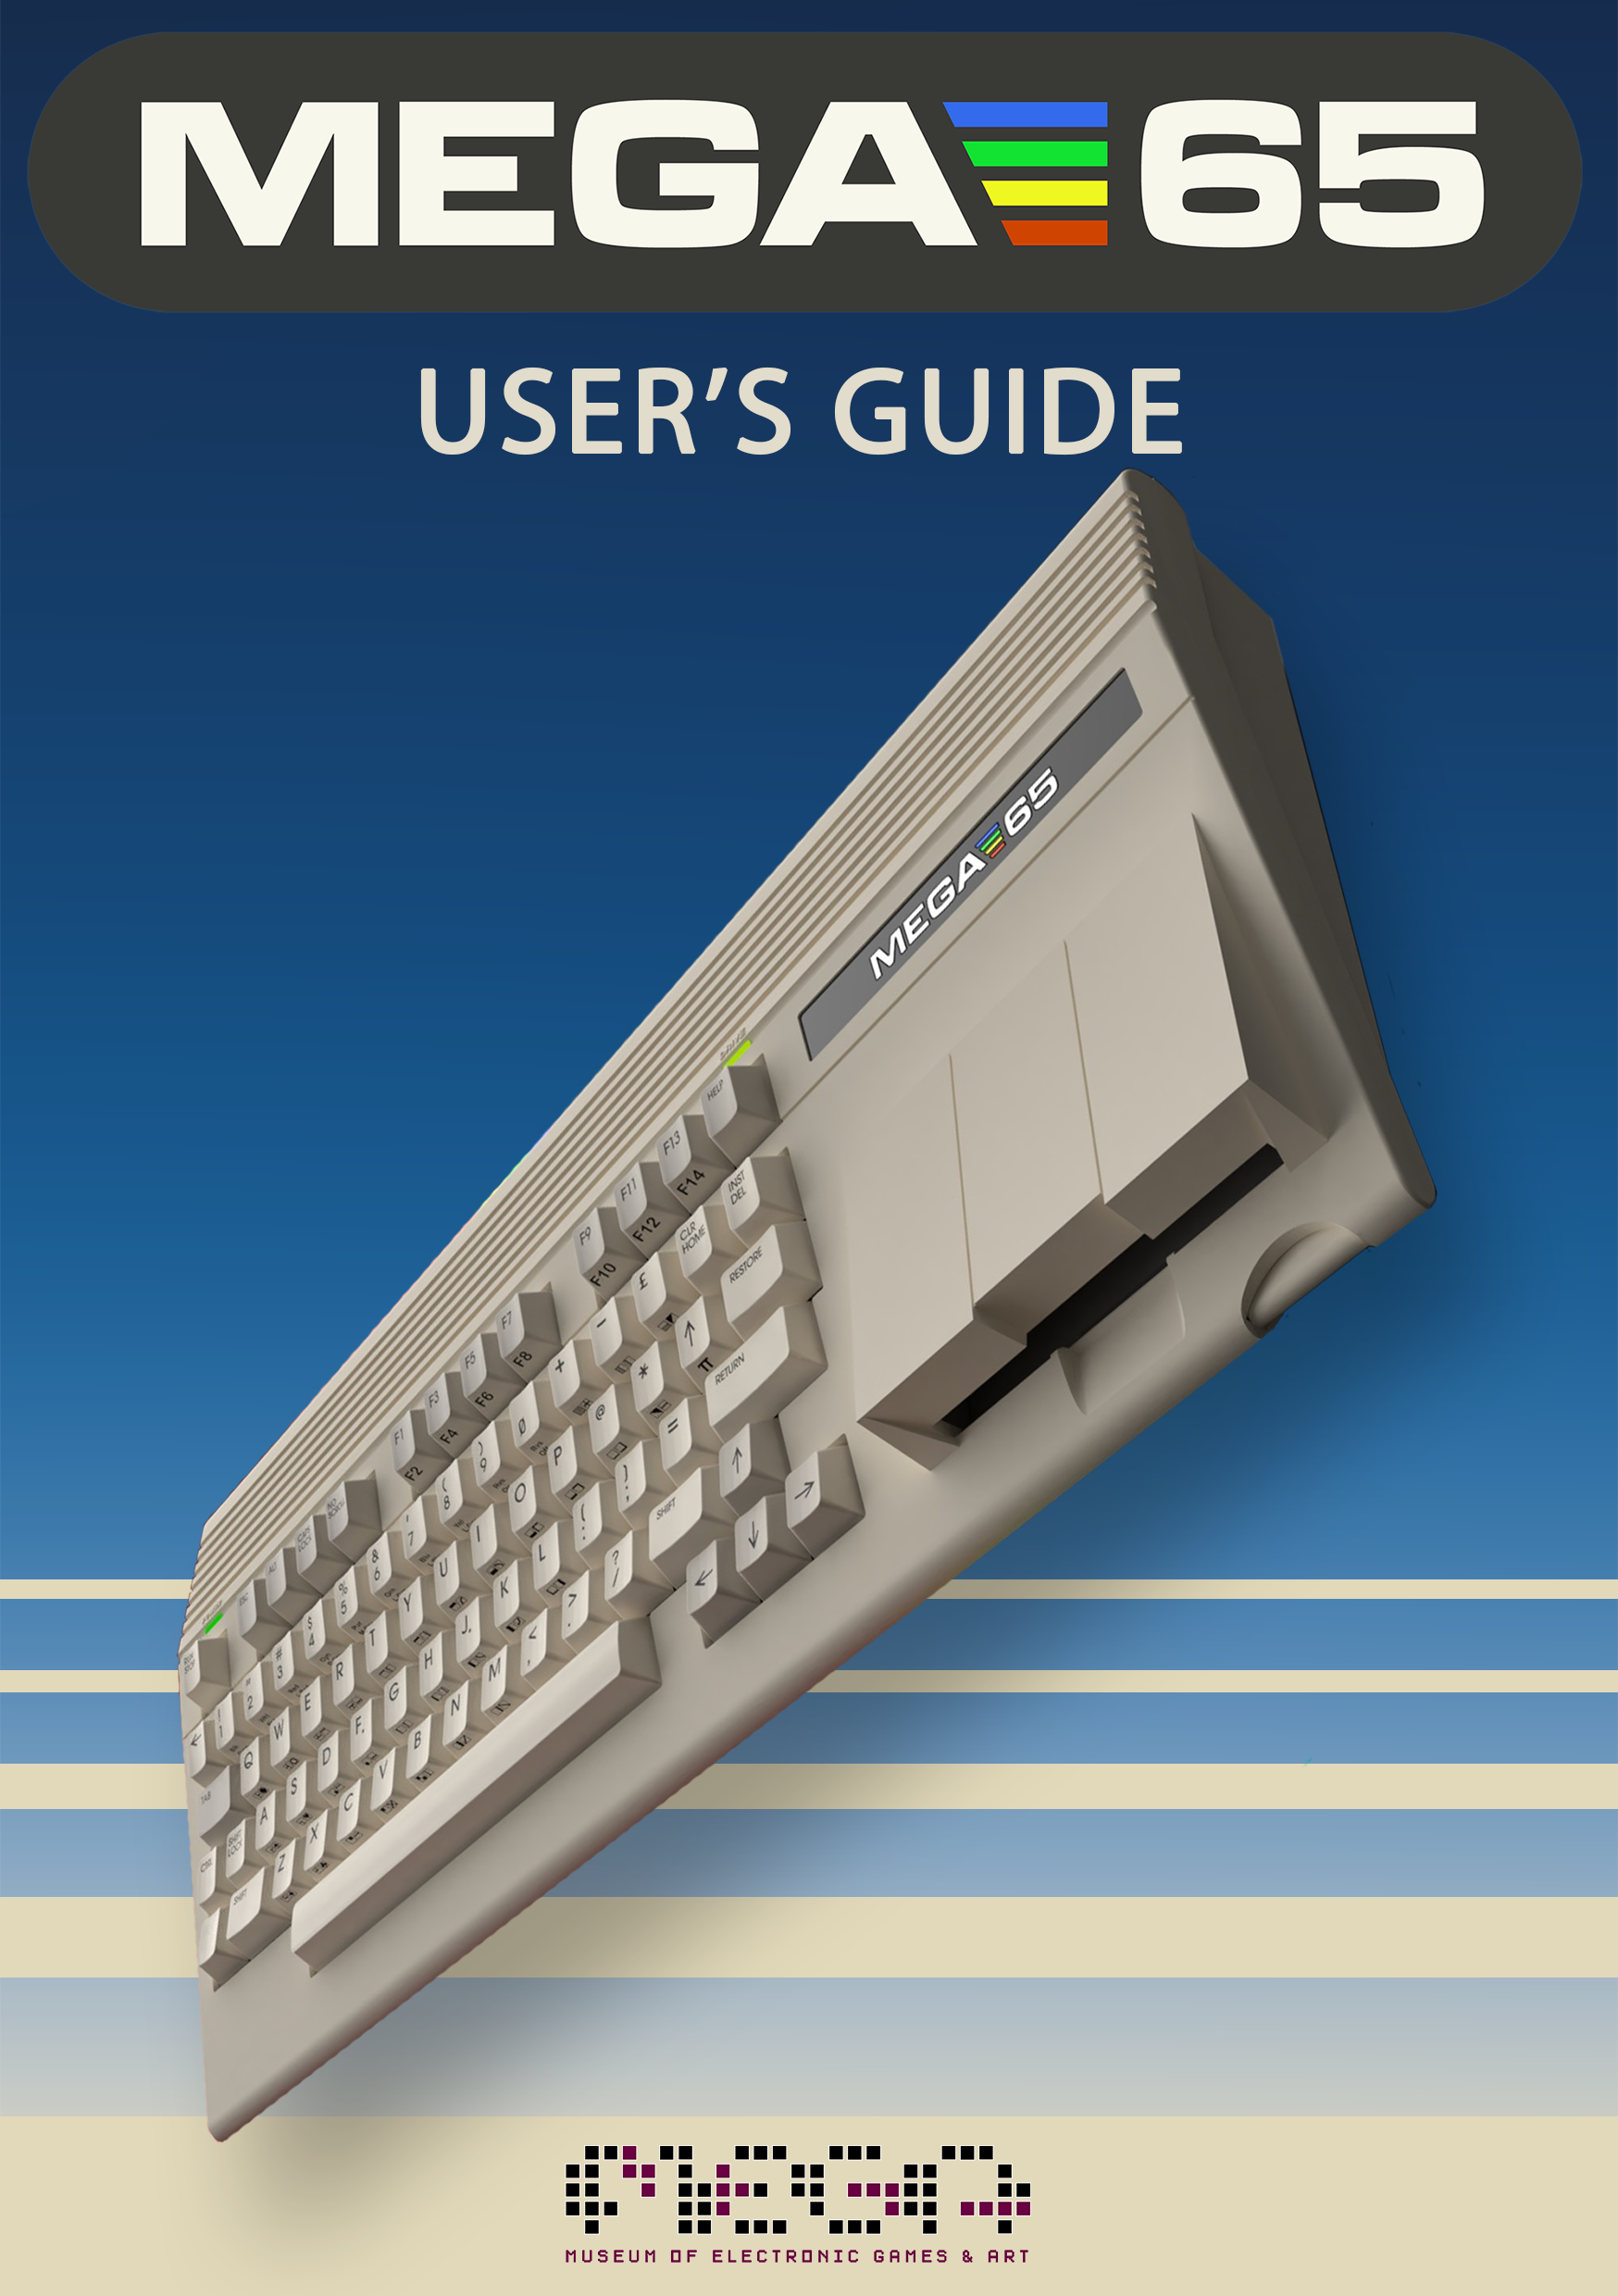
\includegraphics[height=210mm,width=149mm]{frontcover/manual_title}};
\end{tikzpicture}

%\newpage
%\pagecolor{white}

%\vspace*{-2cm}\chapter*{MEGA65 TEAM}
\newpage
{\huge MEGA65 TEAM}\vspace{1cm}

\setlength{\tabcolsep}{1mm}
\begin{tabular}{ll}

{\large\bf Dr. Paul Gardner-Stephen}    & {\large\bf Detlef Hastik} \\
\textit{(highlander)}                   & \textit{(deft)} \\
Founder                                 & Co-Founder \\
Software and Virtual Hardware Architect & General Manager \\
Spokesman and Lead Scientist            & Marketing \& Sales \\
& \\
{\large\bf Martin Streit}               & {\large\bf Anton Schneider-Michallek} \\
 \textit{(seriously)}                   & \textit{(adtbm)} \\
Video and Photo Production              & Hardware Pool Management \\
Tax and Organization                    & Soft-, Hard- and V-Hardware Testing \\
Social Media                            & Forum Administration \\
& \\
{\large\bf Falk Rehwagen}               & {\large\bf Antti Lukats} \\
 \textit{(bluewaysw)}                   & \textit{(antti-brain)} \\
Jenkins Build Automation                & Host Hardware Design and Production \\
GEOS, Hardware Quality Management       & \\
& \\
{\large\bf Dieter Penner}               & {\large\bf Dr. Edilbert Kirk} \\
 \textit{(doubleflash)}                 & \textit{(Bit Shifter)} \\
Host Hardware Review and Testing        & Manual and Tools \\
File Hosting                            & ROM Enhancements \\
& \\
{\large\bf Gábor Lénárt}                & {\large\bf Mirko H.} \\
 \textit{(LGB)}                         & \textit{(sy2002)} \\
Emulator                                & Additional Hardware and Platforms \\
& \\
{\large\bf Farai Aschwanden}            & {\large\bf Thomas Hertzler} \\
 \textit{(Tayger)}                      & \textit{(grumpyninja)} \\
File Base, Tools                        & USA Spokesman \\
Financial Advisory                      & Artist Relations \\
& \\
{\large\bf Andrew Owen}                 & {\large\bf Daniel England} \\
 \textit{(Cheveron)}                    & \textit{(Mew Pokémon)} \\
Keyboard Advisory, Sinclair Support     & Additional Code and Tools \\
& \\
{\large\bf Roman Standzikowski}         & {\large\bf Hernán Di Pietro} \\
 \textit{(FeralChild)}                  & \textit{(indiocolifa)} \\
Open ROMs                               & Additional Emulation \\
\end{tabular}


\chapter*{Reporting Errors and Omissions}

This book is a work-in-progress produced by and for the MEGA65 community.
The version of this edition is:

\input{gitinfo}

We want this book to be the best that it possibly can. So if you see any errors,
find anything that is missing, or would like more information,
please report them using the MEGA65 User's Guide issue tracker:

\url{https://github.com/mega65/mega65-user-guide/issues}

You can also check there to see if anyone else has reported a similar problem,
while you wait for this book to be updated.

Finally, you can always download the latest version of this book from:

\url{https://github.com/mega65/mega65-user-guide}




% paper title
% Titles are generally capitalized except for words such as a, an, and, as,
% at, but, by, for, in, nor, of, on, or, the, to and up, which are usually
% not capitalized unless they are the first or last word of the title.
% Linebreaks \\ can be used within to get better formatting as desired.
% Do not put math or special symbols in the title.

\cleardoublepage

\pagenumbering{roman}

  \begin{titlepage}
    \pagecolor{blue}
     \begin{center}
       {
         \large
         % Put a nice amount of vertical space before the title
         \vspace*{2cm}
               {\Huge\textcolor{white}{\bf{Developing for the MEGA65}}}\\
             \vspace{\fill}
                    {\textcolor{white}
                    {Published by \\ the MEGA Museum of Electronic Games
                    and Art, Germany.\\and\\Flinders University, Australia.}}
       }
     \end{center}
   \end{titlepage}

% Then the copyright notice page
  \pagecolor{white}\textcolor{black}
  \vfill
  WORK IN PROGRESS

  \index{copyright}Copyright \copyright 2019 -- 2020 by Paul Gardner-Stephen,
  Flinders University, the Museum of Electronic Games and Art eV.,
  and contributors.

  This reference guide is made available under the GNU Free Documentation
  License v1.3, or later, if desired. This means that you are free to
  modify, reproduce and redistribute this user guide, subject to
  certain conditions. The full text of the GNU Free Documentation
  License v1.3 can be found at
  \url{https://www.gnu.org/licenses/fdl-1.3.en.html}.

  Implicit in this copyright license, is the permission to duplicate
  and/or redistribute this document in whole or in part for use in
  education environments. We want to support the education of future
  generations, so if you have any worries or concerns, please contact us.

   \par\today

\newpagestyle{onlynumber}{\setfoot[][{\bf\small\thepage}][]
                                  {} {\bf\small\thepage} {}}
\pagestyle{onlynumber}
\pagecolor{white}

\tableofcontents

%% XXX - big numbers are not in bold, because latex gets confused
\newcommand*{\justifyheading}{\raggedleft}
\definecolor{headingblue}{rgb}{0.5,0.5,1}

% \titleformat{command}[shape]
%   {format}
%   {label}
%   {sep}
%   {before}
%   [after]

% ***************
% PART title page
% ***************

\titleclass{\part}{top}
\titleformat{\part}[display]
   {\thispagestyle{empty}\pagecolor{blue}\normalfont\huge\bfseries\justifyheading}
   {\textcolor{white}{\fontsize{50}{65}\selectfont\bf{PART}\quad{\fontsize{100}{130}\selectfont \bf{\serifed\thepart}}}}
   {20pt}
   {\Huge\textcolor{white}}
   [\newpage\pagecolor{white}\textcolor{black}]

% ******************
% CHAPTER title page
% ******************

\titleformat{\chapter}[display]
   {\thispagestyle{empty}\pagecolor{blue}\normalfont\huge\bfseries\justifyheading}
   {\textcolor{white}{\MakeUppercase{\chaptertitlename}\quad{\fontsize{100}{130}\selectfont \bf\thechapter}}}
   {20pt}
   {\Huge\textcolor{white}}
   [{\chapmtoc\insertminitoc}\newpage\pagecolor{white}\textcolor{black}\cleardoublepage]

% ******************
% SECTION title page
% ******************

\titleformat{\section}[display]
   {\raggedright}
   {\thesection}
   {20pt}
   {\huge\bf\color{headingblue}\uppercase}
   [\color{black}]

\chapter{Introduction}

Congratulations on your purchase of one of the most long-awaited computers in the history of computing. The MEGA65 is a community designed computer, based on the never-released Commodore{\textregistered} 65\footnote{Commodore is a trademark of C= Holdings} computer; a computer designed in 1989 and intended for public release in 1990. Decades have passed, and the MEGA 65 invokes an earlier time when computers were simple and friendly. They were not only simple to operate and understand how they work, but friendly and approachable for new users.

These 1980s computers inspired an entire generation of professionals to choose the exciting and rewarding technology careers they have today. Just imagine the joy of these individuals as they learned they could use their new computer to solve problems, write a letter, prepare taxes, invent new things, or even discover how the universe works. We want to recreate that level of excitement not found in modern computing, so we made the {\bf MEGA65}.

The MEGA65 team believes that owning a computer is like owning a home; you don't just use a home; you change things big and small to make it your own custom living space. After a while, when you settle in, you may decide to renovate or expand your home to make it more comfortable or provide more utility. Think of the MEGA65 as a "computing home."

This guide will teach you how to do more than just hang pictures on a wall, it will ask you to build your dream home. While you read this user's guide, you will learn how to operate the MEGA65, code programs, add additional software, and extend hardware capabilities. What won't be immediately obvious is that along the journey, you will also learn about the history of computing as you explore Commodore BASIC version 10 and operating system commands.

Computer graphics and music make computing more fun; and we designed the MEGA65 for fun! In this user's guide, you will learn to code using the MEGA65's built-in {\bf graphics} and {\bf sound} capabilities. But you don't need to be a coder to have fun with the MEGA65. Because the MEGA65 includes a complete Commodore{\textregistered} 64{\texttrademark}\footnote{Commodore 64 is a trademark of C= Holdings, }, it can also run thousands of games, utilities, and business software from the past and new programs being written today by Commodore enthusiasts. Excitement for the MEGA65 will grow as we discover what programmers as they learn about the power and features of this modern Commodore computer recreation. Together, we will create a whole new "home-brew" community to do things that even we didn't think were possible when creating the MEGA65.

We welcome you on this journey! Thank you for becoming a part of the {\bf MEGA65}community of  users, coders, and enthusiasts! Get involved, learn more about your MEGA65, and join us online at:

% I thought a call to action to join the community would be good to add early on. Where will the final online community call home?


\cleardoublepage
\pagenumbering{arabic}

\part{INTRODUCTION}

\chapter{Welcome, and thank you!}

I would like to begin by thanking you for your interest in the MEGA65,
and in developing software to run on it. The success of the MEGA65 as
a fun retro-computing platform depends on there being enough
interesting software for people to run on it.  This requires the
generous work of developers like yourself. So, again, thank you!

But developing for the MEGA65 is not merely a case of giving to the
benefit of others. We have tried hard to create a machine that is as
fun to programme as the Commodore 64, but with some of the barriers
and frustrations worn down somewhat.  That is, it is our intention
that people develop on the MEGA65 because it is fun, and then enjoy
the process.  That is, the journey should very much be the
destination.

Now, in saying that, the MEGA65 is quite new, and we have been flat
out creating the machine. This means that some development tools are
not as ready or as simple or integrated as we would like.  Improving
the tools is also an area where we hope that many of you will enjoy
contributing, so that developing for the MEGA65 can become accessible
to as many people as possible.

If you encounter barriers to your
journey of developing for the MEGA65, please do let us know, and
consider creating solutions that can be shared with others.  This will
help everyone

\chapter{Other Resources}

This book focusses on the process of developing for the MEGA65.  To
avoid it being a thousand pages long, it doesn't describe the inner
workings of the MEGA65, except where you need to know about them, so
that you can engage in the development process.  For example, if you
wish to know about the capabilities of the various custom chips in the
MEGA65, and which registers do which things, please refer to {\em the
MEGA65 Book} online
at \url{https://github.com/mega65/mega65-user-guide}, or consider
purchasing one or more of the reference volumes for the MEGA65, from
which the MEGA65 Book is formed.  For example, the {\em MEGA65 Chipset
Reference Guide} or the {\em MEGA65 Assembly Language Reference Guide}.

We also hope that you, the developer community, will contribute to
those books, or write your own material that can help others in their
journies with developing for the MEGA65.


\part{CROSS-PLATFORM DEVELOPMENT TOOLS}

\chapter{Assemblers}

\chapter{C and C-Like Compilers}

\chapter{BASIC Tokenisers}

\chapter{Data Transfer and Debugging Tools}

\part{NATIVE DEVELOPMENT TOOLS}

\chapter{C65 Memory Monitor}

\chapter{MEGA65 Matrix Mode}

\chapter{Turbo Assembler}

\part{MULTI-MEDIA AND DATA CONVERSION}

\part{GEOS Development}

\part{HARDWARE}

\chapter{Using Nexys4 boards as a MEGA65}

\section{Building your own MEGA65 Compatible Computer}

You can build your own MEGA65-compatible computer by using either a Nexys4DDR (aka. Nexys A7) or the older Nexys4 (Non-DDR) FPGA development boards.
This appendix describes the process to set up a Nexys4DDR (Nexys A7) board for this purpose (which is the newer, preferred board).
The older non-DDR Nexys4 board is also supported, and the instructions are the same, except that
you must use a bitstream designed for that board.
Using a Nexys4DDR bitstream on a non-DDR Nexys4 board, or vice versa, may cause irreparable damage to your board, so make sure
you have the correct bitstream to suit your board.


DISCLAIMER: M.E.G.A cannot take any responsibility for any damage that may occur to your Nexys4DDR/NexysA7/Nexys4 boards.

\newpage

\section{Working Nexys4 Boards}

There are currently 3 Nexys FPGA boards which can be setup as a MEGA65:

\begin{minipage}{\linewidth}
  \subsection{The Nexys4 board}

  No longer manufactured but still available for sale on some websites with old stock.

  \begin{center}
    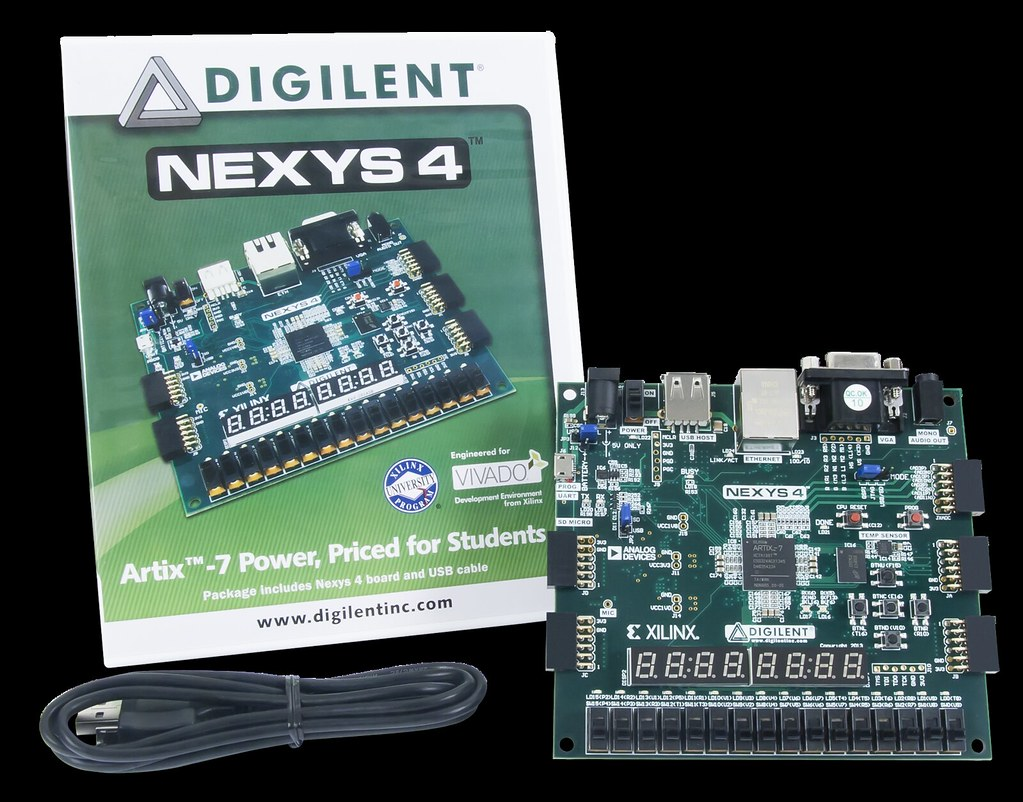
\includegraphics[width=0.4\linewidth]{images/img001_nexys4_board.jpg}
  \end{center}

  Documentation:

  \begin{itemize}
    \item \url{https://reference.digilentinc.com/reference/programmable-logic/nexys-4/reference-manual}
    \item \url{https://reference.digilentinc.com/\_media/reference/programmable-logic/nexys-4/nexys4\_rm.pdf}
  \end{itemize}
\end{minipage}

\begin{minipage}{\linewidth}
  \subsection{The Nexys4DDR board}

  No longer manufactured but still available for sale on some websites with old stock.

  \begin{center}
    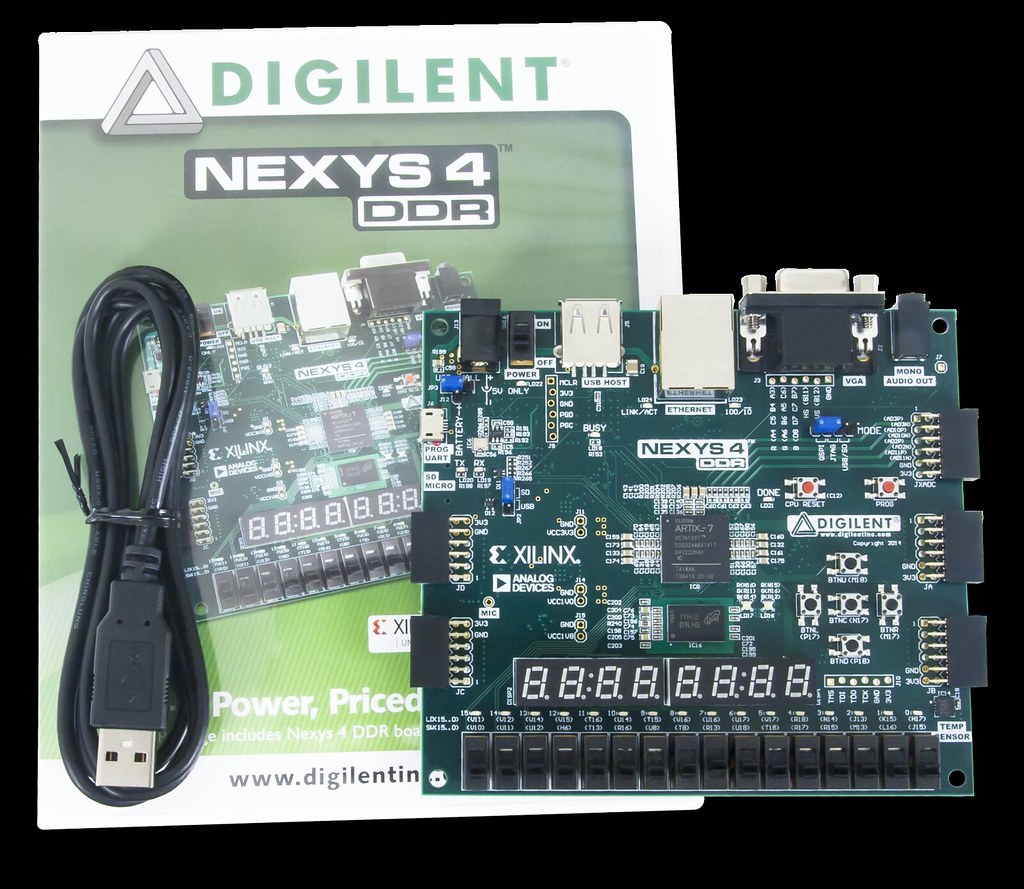
\includegraphics[width=0.4\linewidth]{images/img002_nexys4_ddr_board.jpg}
  \end{center}

  Documentation:

  \begin{itemize}
    \item \url{https://reference.digilentinc.com/reference/programmable-logic/nexys-4-ddr/reference-manual}
    \item \url{https://reference.digilentinc.com/\_media/reference/programmable-logic/nexys-4-ddr/nexys4ddr\_rm.pdf}
  \end{itemize}
\end{minipage}

\begin{minipage}{\linewidth}
  \subsection{The Nexys A7}

  This is the re-branded version of the above Nexys4 DDR board:

  \begin{center}
    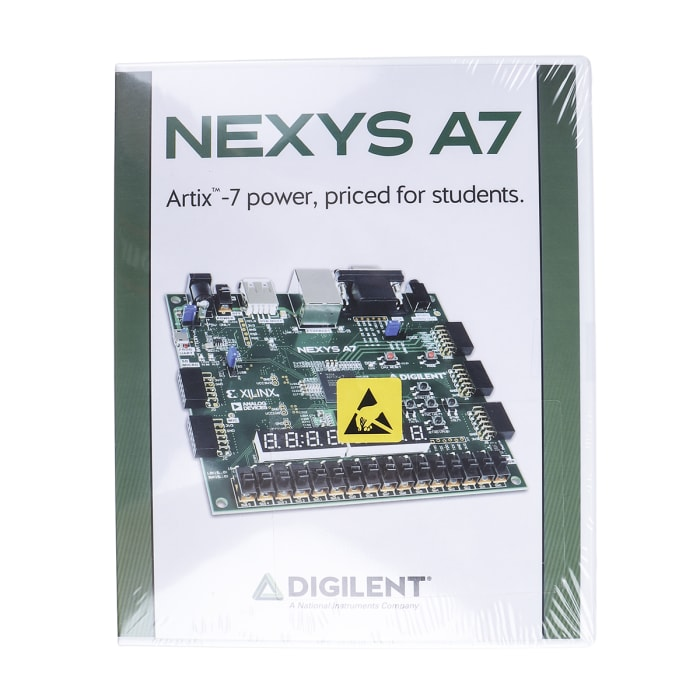
\includegraphics[width=0.4\linewidth]{images/img003_nexysA7_board.jpg}
  \end{center}

  Documentation:

  \begin{itemize}
    \item \url{https://reference.digilentinc.com/reference/programmable-logic/nexys-a7/reference-manual}
    \item \url{https://reference.digilentinc.com/\_media/reference/programmable-logic/nexys-a7/nexys-a7\_rm.pdf}
  \end{itemize}
\end{minipage}

\newpage

\section{Power, Jumpers, Switches and Buttons}

This top-down picture highlights the key jumper positions of interest on the Nexys4 board:

  \begin{center}
    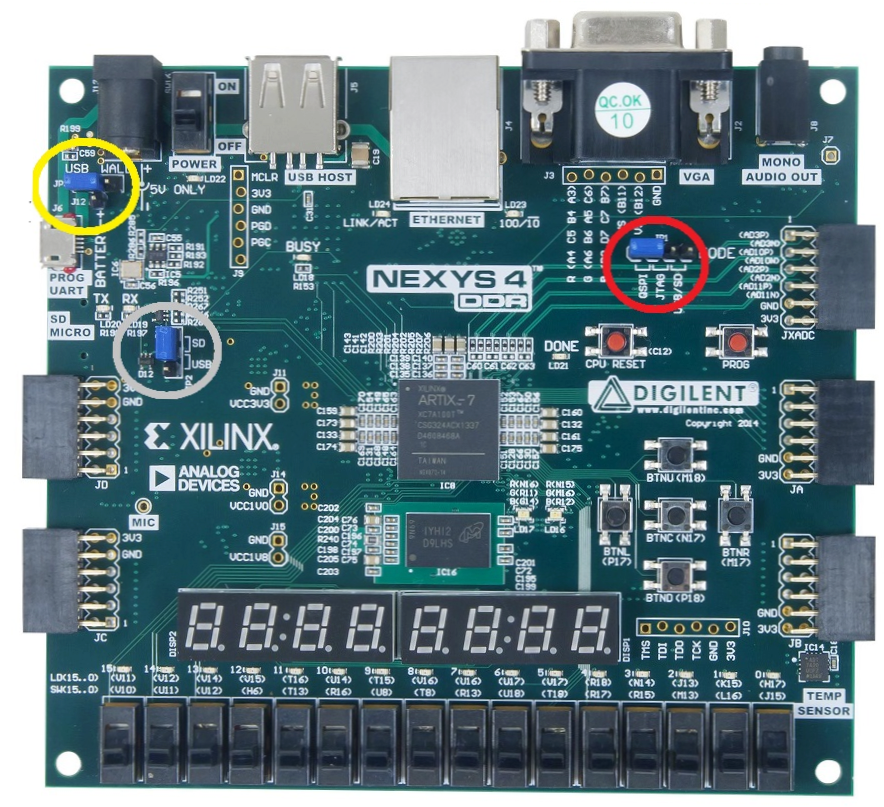
\includegraphics[width=0.9\linewidth]{images/nexys4_jumpers.png}
  \end{center}

The Nexys4 boards can be powered in two ways: using an external power supply, or from a standard USB port.

\subsection{Micro-USB Power}

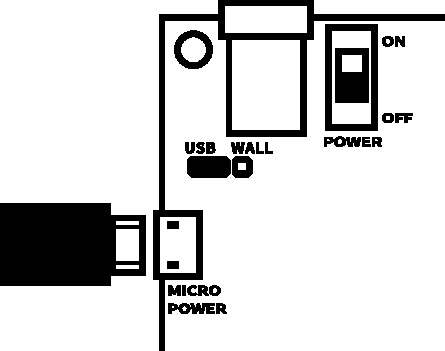
\includegraphics[width=5cm]{images/illustrations/nexys-micro-usb-power.pdf}

Connect your micro-usb cable to a USB port on a USB charger or PC to provide power. Connect the other end to the Nexys4's micro-usb connector. Place the JP3 jumper on pins 1 and 2 to select USB power. Use the switch to power up the Nexys4.

\subsection{External Power Supply}

\hspace*{1.7cm}
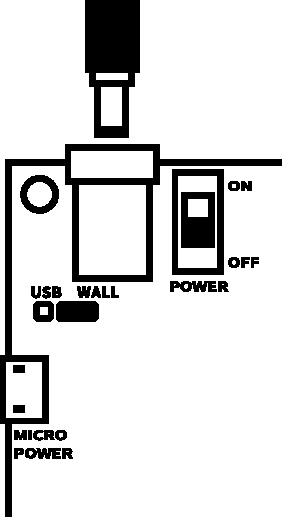
\includegraphics[width=3.2cm]{images/illustrations/nexys-power-supply.pdf}

The MEGA65 core can consume a lot of power, and a standard USB port could potentionally be too little for the Nexys4 board. In particular, writing to the SD card might hang or perform odd behaviour. Therefore you should consider a 5V power supply.

Digilent sell a power supply for the Nexys4 board, and we recommend you use this to ensure you avoid the risk of damage to your Nexys4 board. The chosen power supply should be center positive, 2.1mm internal diameter plug, and should deliver 4.5VDC to 5.5VDC rated at least 1 Amp.

Connect the power supply cable to the supply plug of the Nexys4. Place the JP3 jumper on pins 2 and 3 to select WALL power. Use the switch to power up the Nexys4.

\subsection{Other Jumpers and Switches}

For your initial set up, we'd suggest you set the following jumpers on your Nexys4 board to these positions:

\begin{itemize}
  \item{JP1} - USB/SD
  \item{JP2} - SD
\end{itemize}

\begin{center}
  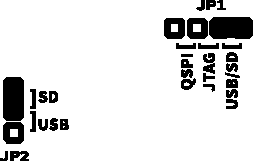
\includegraphics[width=3.2cm]{images/illustrations/nexys-jumpers.pdf}
\end{center}

This will assure that the bitstream files will get loaded from your SD card on start-up.

At some later stage, you may prefer to load the bitstream from the on-board QSPI flash, and at that point, you can revisit your JP1 jumper setting and adjust it to the QSPI position.

% XXX - Image of board highlighting the jumpers

All 16 switches on the lower edge of the board must be set to the off position.


\subsection{Connections and Peripherals}

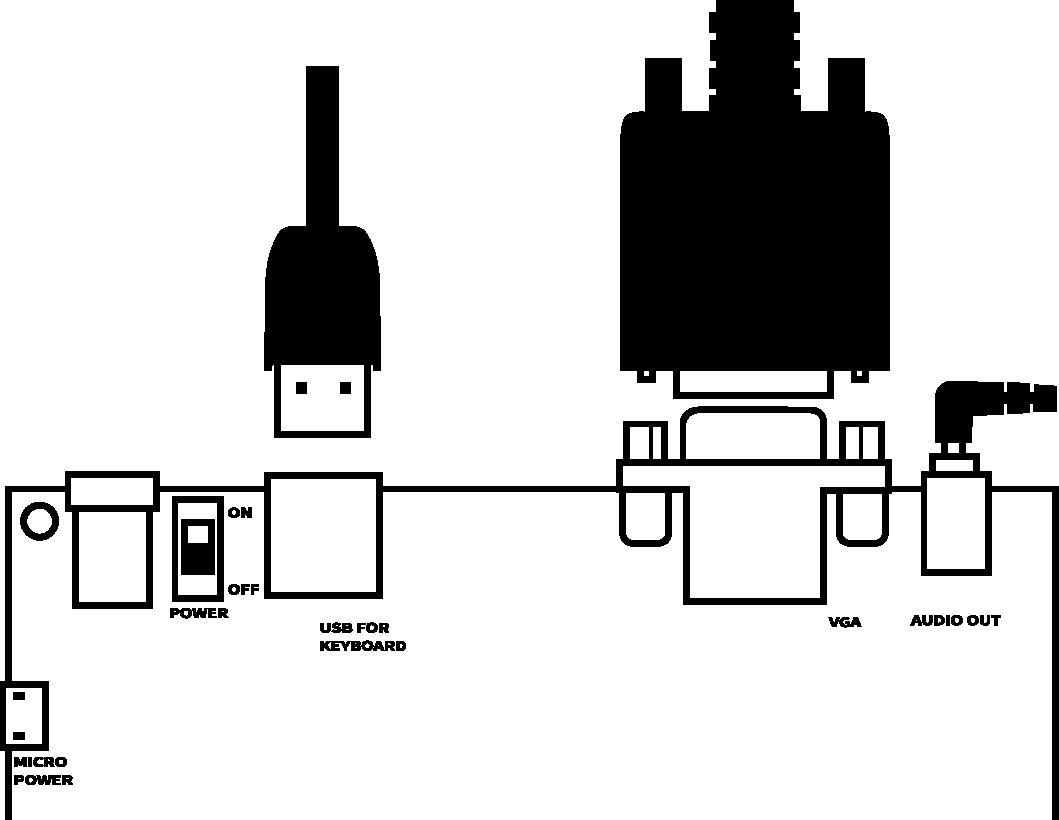
\includegraphics[width=\linewidth]{images/illustrations/nexys-connectors.pdf}

A USB keyboard can be connected to the USB port. Only a keyboard that lacks a USB hub will work with the Nexys4 board.  Generally, extremely cheap keyboards will work, while more expensive keyboards tend to have a USB hub integrated, and will not work.  You may need to try several keyboards before you find one that works.

You can connect a VGA monitor to the VGA port.

The mono audio-out jack can be connected to the line-in of an amplifier.


\subsection{Communicating with your PC}

There may be occasions where you wish to communicate with your Nexys4 board from your PC, in order to perform activities such as:

\begin{itemize}
  \item Flash your QSPI flash chip via Vivado
  \item Upload bitstream files directly from your PC (via m65 tool)
  \item Make use of support tools such as M65Connect, m65, mega65\_ftp, m65dbg, etc
\end{itemize}

On such occasions, you will need to connect your micro-usb cable up to your PC.

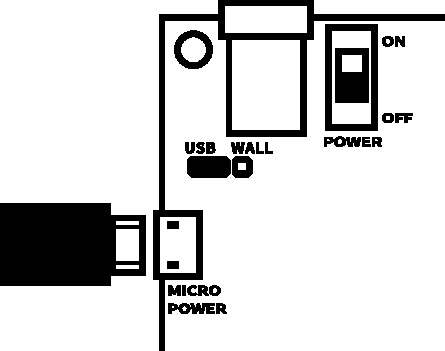
\includegraphics[width=5cm]{images/illustrations/nexys-micro-usb-power.pdf}

\subsection{Onboard buttons}

\begin{center}
  
\includegraphics[width=3.2cm]{images/illustrations/nexys-reset-buttons.pdf}
\end{center}

The ``CPU RESET'' button will reset the MEGA65 when pressed, while the ``PROG'' button will cause the FPGA itself to reload the MEGA65
core.  The main difference between the two is that CPU RESET is faster, and does not clear the contents of memory, while the FPGA button
is slower, and does reset the contents of memory.

\begin{center}
  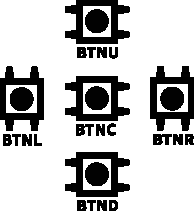
\includegraphics[width=3.2cm]{images/illustrations/nexys-five-buttons.pdf}
\end{center}

Two of the five buttons in the cross arrangement can also be used:  BTND acts as though you have pressed \widekey{RESTORE}, while BTNC will trigger an IRQ, as though the IRQ line had been pulled to ground.

\section{Keyboard}

The keyboard layout is positional rather than logical.
This means that keys in similar positions to the keys on a C65 keyboard will have similar function.
This relationship assumes that your USB keyboard uses a US keyboard layout.

To help you locate what the various MEGA65 keys are mapped to, the MEGA65 has a built-in virtual keyboard test feature. This can be accessed in two ways.

The easiest way is to keep \specialkey{ALT} held down in while switching on the Nexys4, or resetting the Nexys4 with
the ``PROG'' button. The configure menu will be presented and by pressing 3, the virtual keyboard will be presented on a black background.

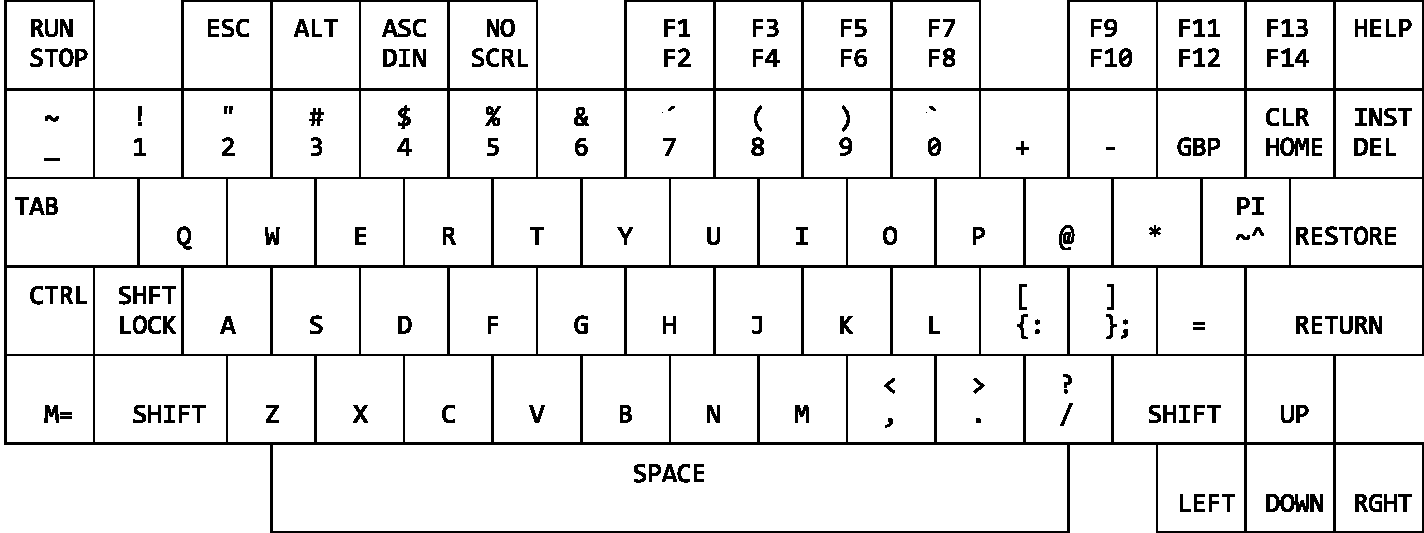
\includegraphics[width=\linewidth]{images/illustrations/virtual-keyboard.pdf}

Pressing a key on the USB keyboard will show the highlighted key on the virtual keyboard to help you identify the key mapping.

The other way to access the virtual keyboard is from within the MEGA65. Hold \megasymbolkey and press \specialkey{TAB} to access the Matrix Mode Debugger. From here, enter the following:

\screentextwide{s ffd3615 ff}

This will open a semi-transparent virtual keyboard at the top of the screen. Alternatively:

\screentextwide{s ffd3615 ff ff}

This will open a semi-transparent virtual keyboard in the centre of the screen.

Hold \megasymbolkey and press \specialkey{TAB} to exit Matrix Mode Debugger and return to the MEGA65.

\subsection{Some key mappings with a USB keyboard}

\widekey{RESTORE} is mapped to the PAGE UP key.

\specialkey{RUN STOP} is mapped to \specialkey{ESC}.

\newpage

\section{Preparing microSDHC card}

The MEGA65 requires an SDHC card of between 4GB and 64GB capacity.  Some SDXC cards may work, however, this is not officially supported.

Preparation steps for the Nexys4 board's SD card share much in common with the steps needed for real MEGA65 hardware, and as such, it is worth having a look over the \nameref{cha:configuring} chapter if you ever need details.

So in this section, we'll provide more details on the distinctive steps, and be more brief on the common steps.

One point of distinction between the Nexys board and the real MEGA65 hardware is that the latter already has a default bitstream/core provided, which permits you to format your SD card in the specific style required by the MEGA65.

For Nexys4 board owners however, you have no such default bitstream, so
see \nameref{sec:bitstreamfiles} for more details on where the appropriate "nexys4.bit" or "nexys4ddr-widget.bit" files for your device can be downloaded from.

\subsection{Preparation Steps}

The steps are:

\begin{itemize}
  \item{Format the SD card} in a convenient computer using the FAT32 file-system.  The MEGA65 and Nexys4 boards do not understand other
file systems, especially the exFAT file system.
\item{Copy} your bitstream file (with name ending in ``.bit'') onto the SD card.
\item{Insert} the SD card into the SD card slot on the under-side of the Nexys4 board.
\item{Switch on} the Nexys4 board.
\item{Enter the Utility Menu} by holding \specialkey{ALT} down on the USB keyboard you have connected to the Nexys4 board.
\item{Enter the FDISK/FORMAT tool} by pressing 2 when the option appears on the MEGA65 boot screen.
\item{Follow the prompts} in the FDISK/FORMAT program to again format the SD card for use by the MEGA65. \\
  \\
  The FDISK tool will partition your SD card into two partitions and format them.
  \begin{itemize}
    \item One is type \$41 = MEGA65 System Partition, where the save slots, configuration data and other files live. \\
  (This partition is invisible in i.e. Win PCs).
    \item The other partition with type \$0C = VFAT32, where KERNAL, support files, games, and so on, will be copied to later. \\
  (This partition is visible on i.e. Win PCs).
  \end{itemize}
\item{Once formatting is complete}, switch off the Nexys4 board and remove the microSDHC card from the Nexys board and put it back into your PC
\item{This time, copy} the following items onto the SD card:
  \begin{itemize}
    \item The bitstream file
    \item The extracted files from within either the "\textbf{SD essentials.rar}" or "\textbf{SD essentialsNoROM.rar}" file that you downloaded from the MEGA65 filehost. (See \nameref{sec:installingrometc} for more details).
    \item{If you have sourced your own preferred ROM file} (e.g. "\textbf{911001.BIN}"), copy it onto the SD card also, and rename it to "\textbf{MEGA65.ROM}" (uppercase is essential).
    \item{Any .D81 disk image files} you wish to make use of.
      \begin{itemize}
        \item Note that if a file named MEGA65.D81 is added to the SD card, it will be mounted automatically on startup.
        \item Make sure that all .D81 files have names that fit the old DOS 8.3 character limit, and are upper case.  This restriction will be removed in a future release.
      \end{itemize}
  \end{itemize}
\item{Remove the SD card} and reinsert it into your Nexys4 board.
\item{Power the Nexys4} board back on.  The MEGA65 should boot within 15 seconds.
\item On first start up, you will find yourself at the on-boarding screen, of which more details can be found in the \nameref{cha:configuring} chapter.

\end{itemize}

Congratulations. Your MEGA65 has been set up and is ready to use.

Please note that the above method of copying the bitstream file to the SD card means that the bitstream is loaded into the Nexys FPGA each time on boot - which takes around 13 seconds for the system to start. The bitstream can also be flashed using Vivado software into the QSPI flash to deliver a boot up time of 0.3 seconds. 

For more detailed information on preparing and configuring your MEGA65, please refer to the \nameref{cha:configuring} chapter. 

\section{Loading the bitstream from QSPI}

While loading the bitstream from the SD card is the suggested (and well-trodden) path this document has chosen, of late, more nexys4 users have been exploring the alternative pathway of loading the bitstream from the QSPI flash. Some potential reasons they have chosen this pathway are:

\begin{itemize}
  \item Faster loading times (0.3 seconds versus 13 seconds)
  \item Some people were interested in the possibility of flashing multiple cores onto their QSPI (via steps described in the \nameref{cha:cores} Chapter)
  \item Some people have experienced niggling issues with the SD card pathway, such as:
    \begin{itemize}
      \item System unable to reboot from on-boarding screen
      \item System unable to reboot from freeze-menu after switching between PAL/NTSC
    \end{itemize}
\end{itemize}

In time, if this proves to be a more popular pathway, we can revise our documentation here to suit it. Here are some steps in brief.

\subsection{Preparation Steps}

For users that want to try this pathway, you will need to adjust the JP1 jumper setting to use QSPI and then follow the steps in the \nameref{cha:fpgacpldflashing} chapter in relation to \nameref{sec:installvivado} and \nameref{sec:mainfpgaflashing}.

Be forewarned that the installation of Vivado is a lengthy process (both in terms of download time, and installation time).

Once you have flashed Slot0 of your QSPI chip via Vivado, you can then follow the steps described in \nameref{cha:configuring} to perform the custom SD card formatting, installing of ROM and support files and on-boarding.

\section{Useful Tips}

The following are some useful tips for getting familiar with the MEGA65:

\begin{itemize}

\item{Press \& hold \megasymbolkey (or the Commodore key if using a Commodore 64 or 65 keyboard) during boot to start up in C64-mode instead of C65-mode}
 \item{Press \& hold \specialkey{RUN STOP} during boot to enter the machine language monitor, instead of starting BASIC.}
\item{Press \widekey{RESTORE} for approximately 1/2 - 1 second to enter the MEGA65 Freeze Menu.  From this menu
  you have convenient tools to change the CPU speed, switch between PAL \& NTSC video mode, change Audio settings, manage freeze-states,
   select D81 disk images, examine and modify memory of the frozen program, among other features.  This is in many ways the heart of the MEGA65, so it is well worth exploring and getting familiar with.}
\item{Type \screentext{POKE0,65} in C64-mode to switch  the CPU to full speed (40MHz). Some software may behave incorrectly in this mode, while other software will work very well, and run many times faster than on a C64.}
\item{Type \screentext{POKE0,64} in C64-mode to switch the CPU to 1MHz.}
\item{Type \screentext{SYS58552} in C64-mode to switch to C65-mode.}
\item{Type \screentext{GO64} in C65-mode and confirm, by pressing \screentext{Y}, to switch to C64-mode, which is the
same as on a C128.}
\item{The C65 ROM makes device 8 the default, so you can normally leave off the \textbf{,8} from the end of LOAD and SAVE commands.}
\item{Pressing \specialkey{SHIFT} + \specialkey{RUN STOP} from either C64 or C65-mode will attempt to boot from disk.}
\end{itemize}

Have fun! The MEGA65 has been lovingly crafted over many years for your enjoyment. We hope you have as much fun using it as we have had creating it!

The MEGA Museum of Electronic Games \& Art welcomes your feedback, suggestions and contributions to this open-source digital heritage preservation project.


\part{APPENDICES}

\begin{appendices}

  \chapter{Flashing the FPGAs and CPLDs in the MEGA65}
\label{cha:fpgacpldflashing}

The MEGA65 is an open-source and open-hardware computer. This means you are free,
not only to write programs that run on the MEGA65 as a finished computer, but you can
use the re-programmable chips in the MEGA65 to turn it into all sorts of other things!

If you just want to install an upgrade core for the MEGA65, or a core that lets you use
your MEGA65 as another type of computer, you are probably looking for Chapter \ref{cha:cores} instead.
This chapter is more intended for people who want to help develop cores for the MEGA65.

These re-programmable chips are called Field Programmable Gate Arrays (FPGAs) or
Complex Programmable Logic Devices (CPLDs), and can implement a wide variety of circuits.
They are normally programmed using a programming language like VHDL or Verilog.  These
are languages that are not commonly encountered by most people.  They are also quite
different in some ways to ``normal'' programming languages, and it can take a while to
understand how they work, but with some effort and perseverance, many people will be
able to do exiting things with them.

Be prepared to install many gigabytes of software on a Linux or Windows PC, before you will
be able to write programs for the FPGAs and CPLDs in the MEGA65.  Also, ``compiling'' complex
designs can take up to several hours, depending on the speed and memory capacity of your computer!
We recommend a computer with at least 8GB RAM, and preferably 16GB if you want to write
programs for FPGAs and CPLDs. If on the other hand all you want to do is load programs onto
your MEGA65's FPGAs and CPLDs that other people have written, then most computers running a recent
version of Windows or Linux should be able to cope.

\section{Warning}

Before we go any further, we do have to provide a warning about reprogramming the FPGAs and
CPLDs in the MEGA65.
Re-programming the MEGA65 FPGA can potentially cause
damage, or leave your MEGA65 in an unresponsive state from which it is very difficult to
recover, i.e., ``bricked''.  Therefore if you choose to open your MEGA65 and reprogram
any of the FPGAs it contains, it is no longer possible to guarantee its correct operation.
Therefore in this case we can not reasonably honour the warranty of the device as a computer.
You have been warned!

\section{Flashing the Artix 100T main FPGA with XILINX VIVADO}

If you choose to proceed, you will need a TE0790-03 JTAG programming module, a functioning
installation of Xilinx's Vivado software.  This can be done on either Windows or Linux, but
in both cases you will need to install any necessary USB drivers. It is also necessary to have
dip-switches 1 and 3 in the ON position and dip-switches 2 and 4 in the OFF position on the TE-0790.
With your MEGA65 disconnected from the power, the TE-0790 must be installed on the JB1 connector,
which is located between the floppy data cable and the audio jack.
The gold-plated hole of the TE-0790 must line up with the screw
hole below.  The mini-USB cable will then connect on the side towards the 3.5" floppy drive.
The following image shows the correct position: The TE0790 is surrounded by the yellow box,
and the dip-switches by the red box. Dip-switch 1 is the one nearest the floppy data cable.


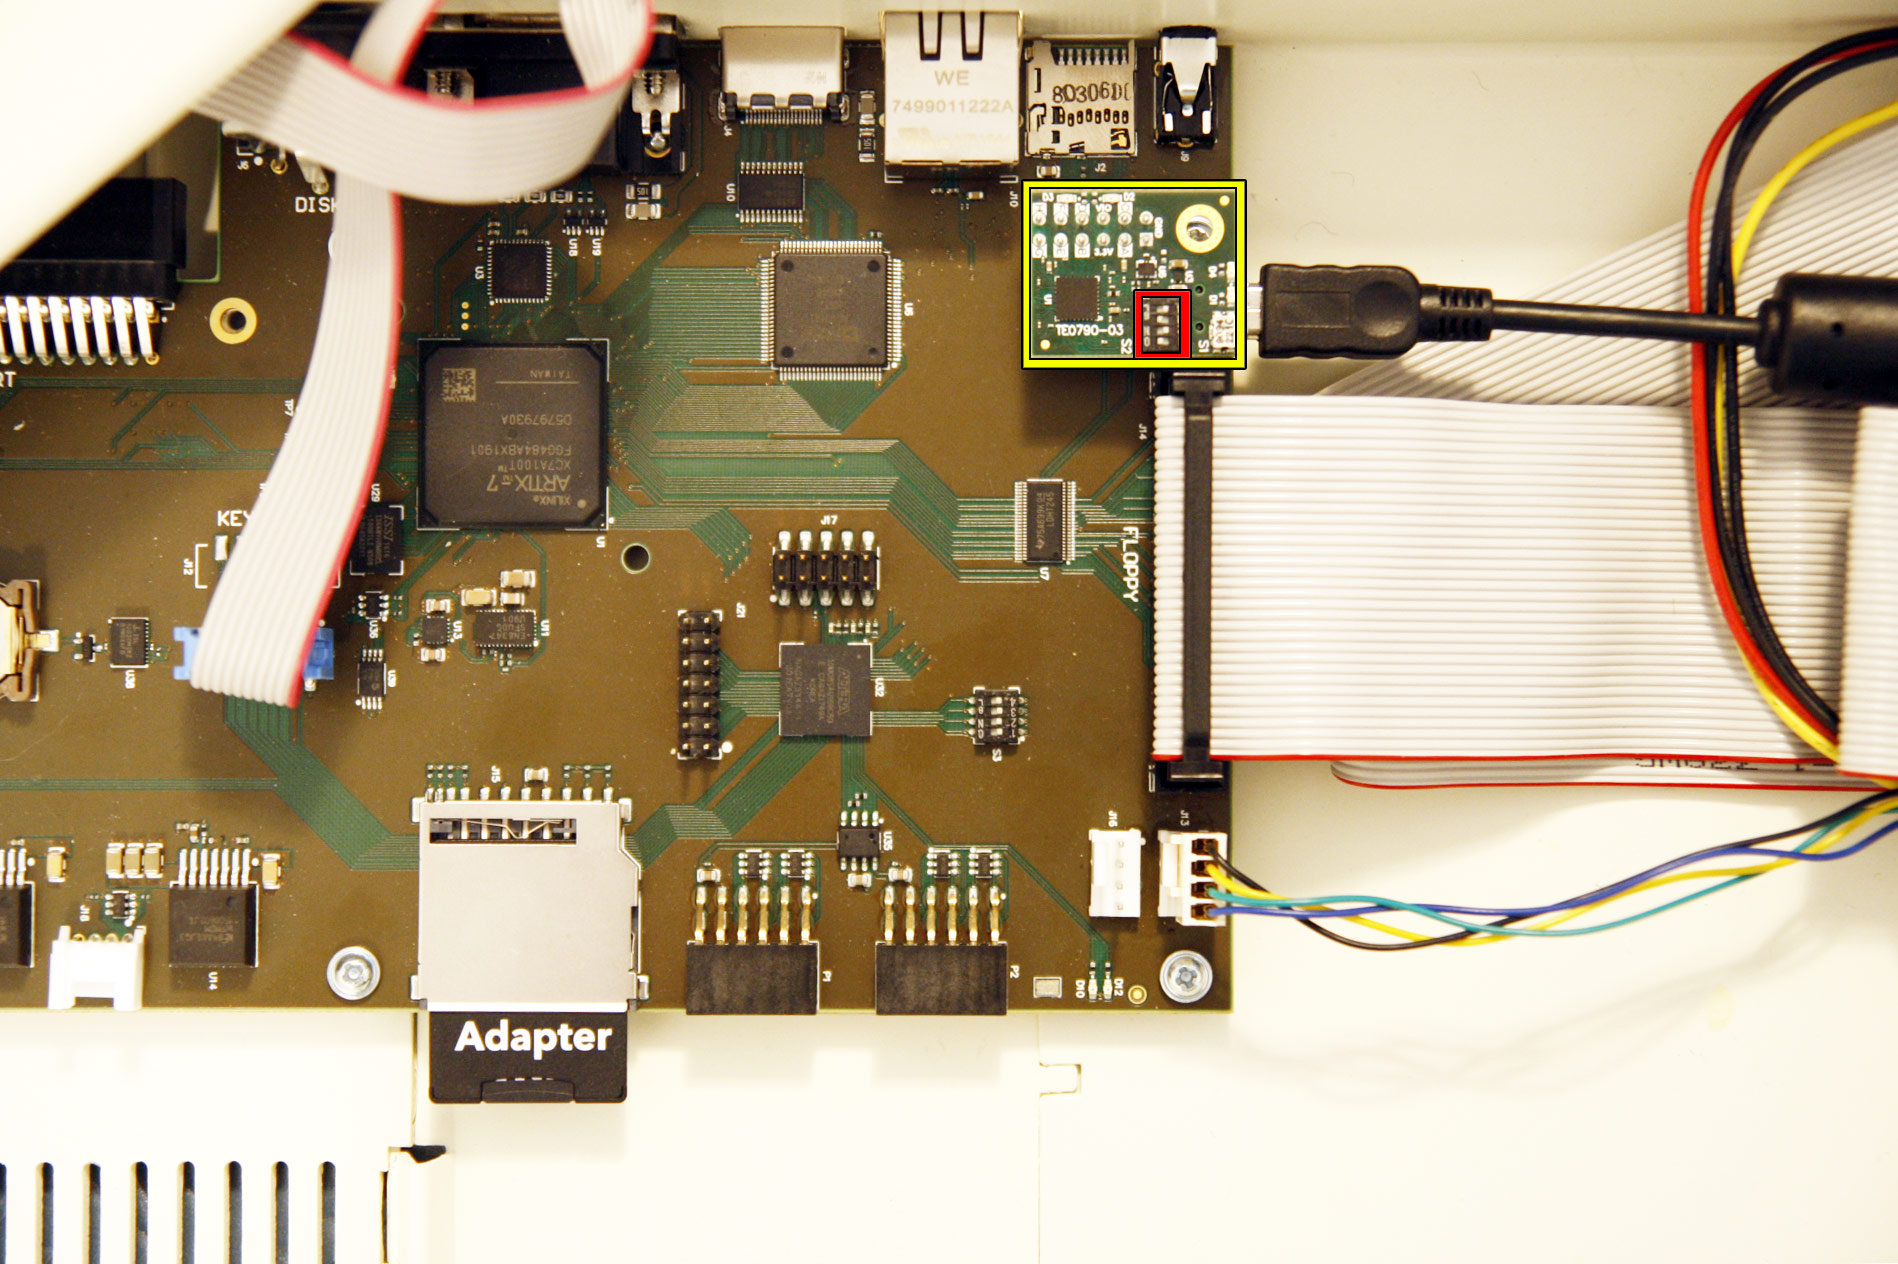
\includegraphics[width=\linewidth]{images/jtag_detail_02.jpg}


Connect your non-8-bit computer to the FPGA programming device using a mini-USB cable. Switch
the MEGA65 computer ON. Open VIVADO, which can be downloaded from the internets.

\begin{figure}
  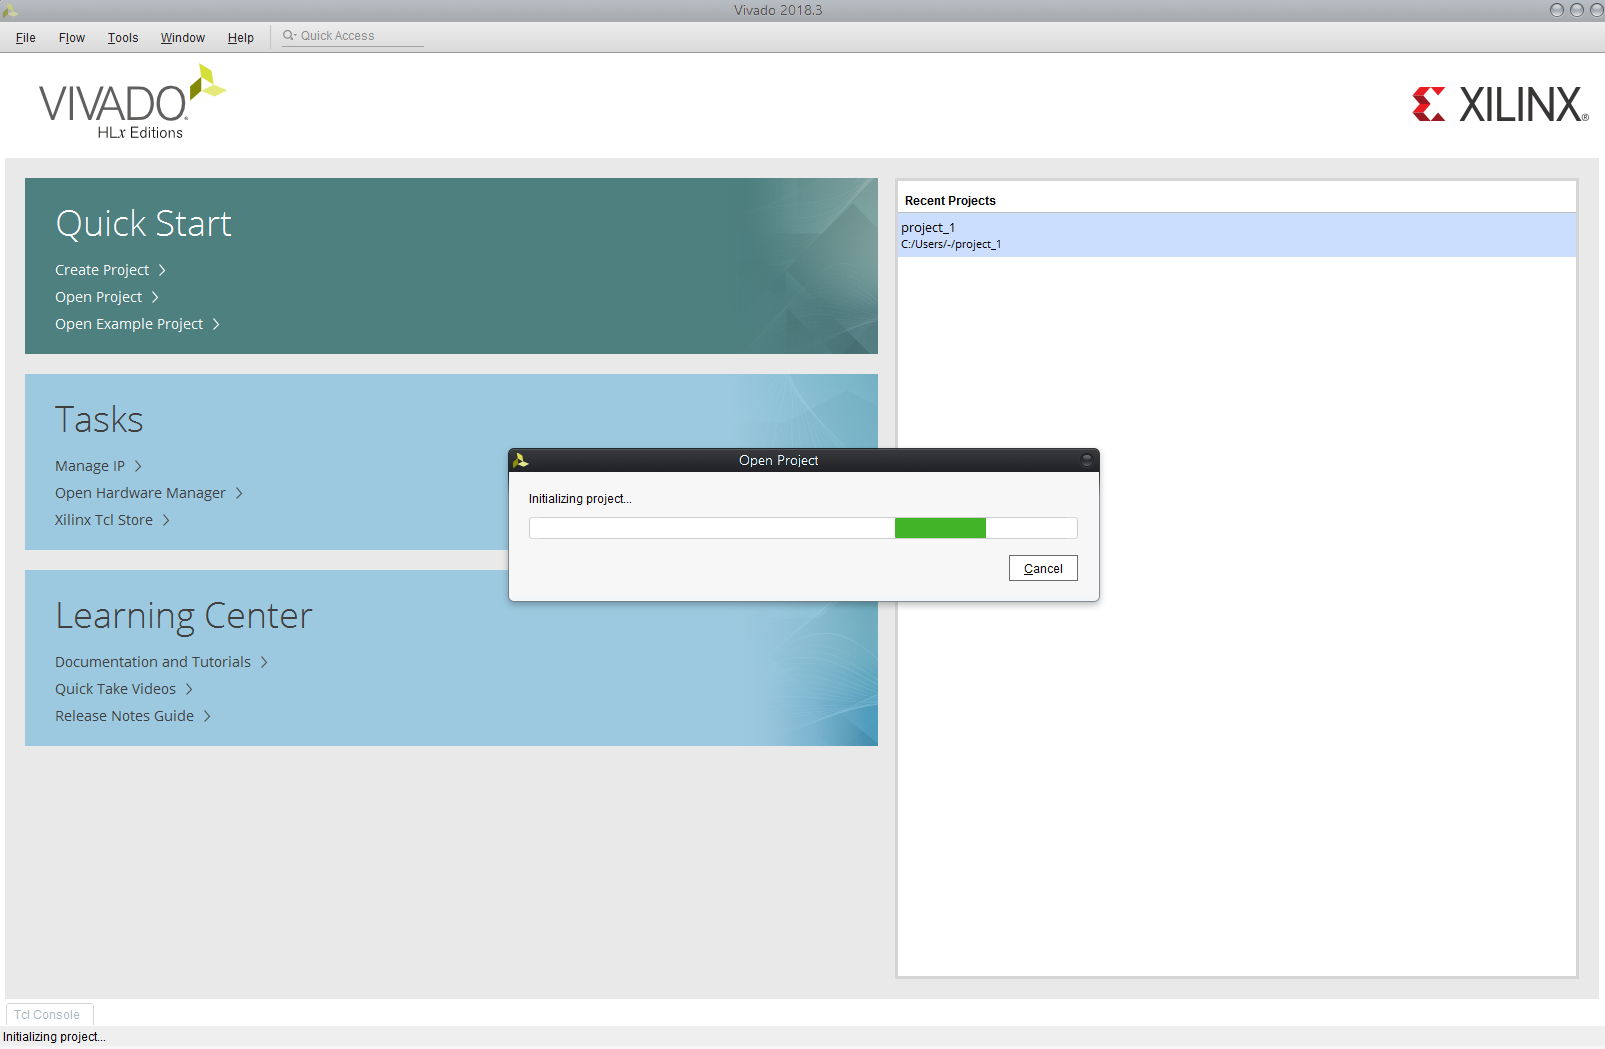
\includegraphics[width=\linewidth]{images/vivado01.png}
  \caption{Step 1: Open a project in VIVADO}
  \label{fig:vivado01}
\end{figure}

To access the Hardware Manager, open a project in VIVADO or create an empty one, if you do not have any projects yet.

\begin{figure}
  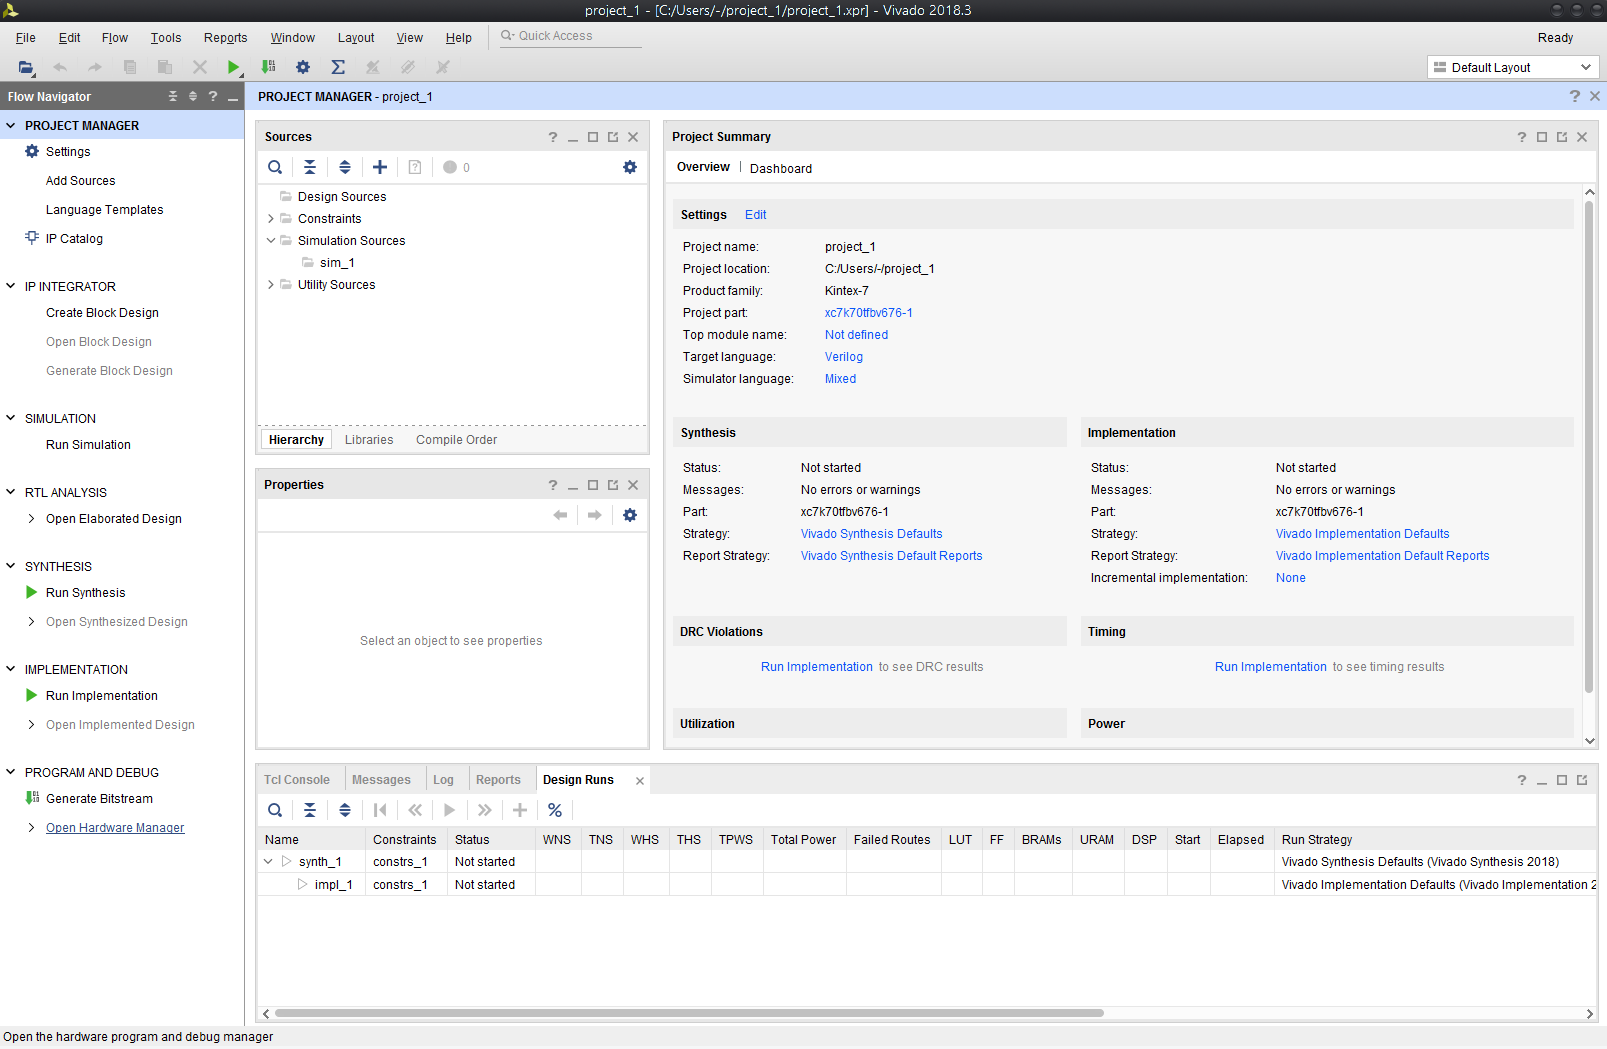
\includegraphics[width=\linewidth]{images/vivado02.png}
  \caption{Step 2: Open Hardware Manager}
  \label{fig:vivado02}
\end{figure}

In the left column, select "Open Hardware Manager" at the very bottom.

\begin{figure}
  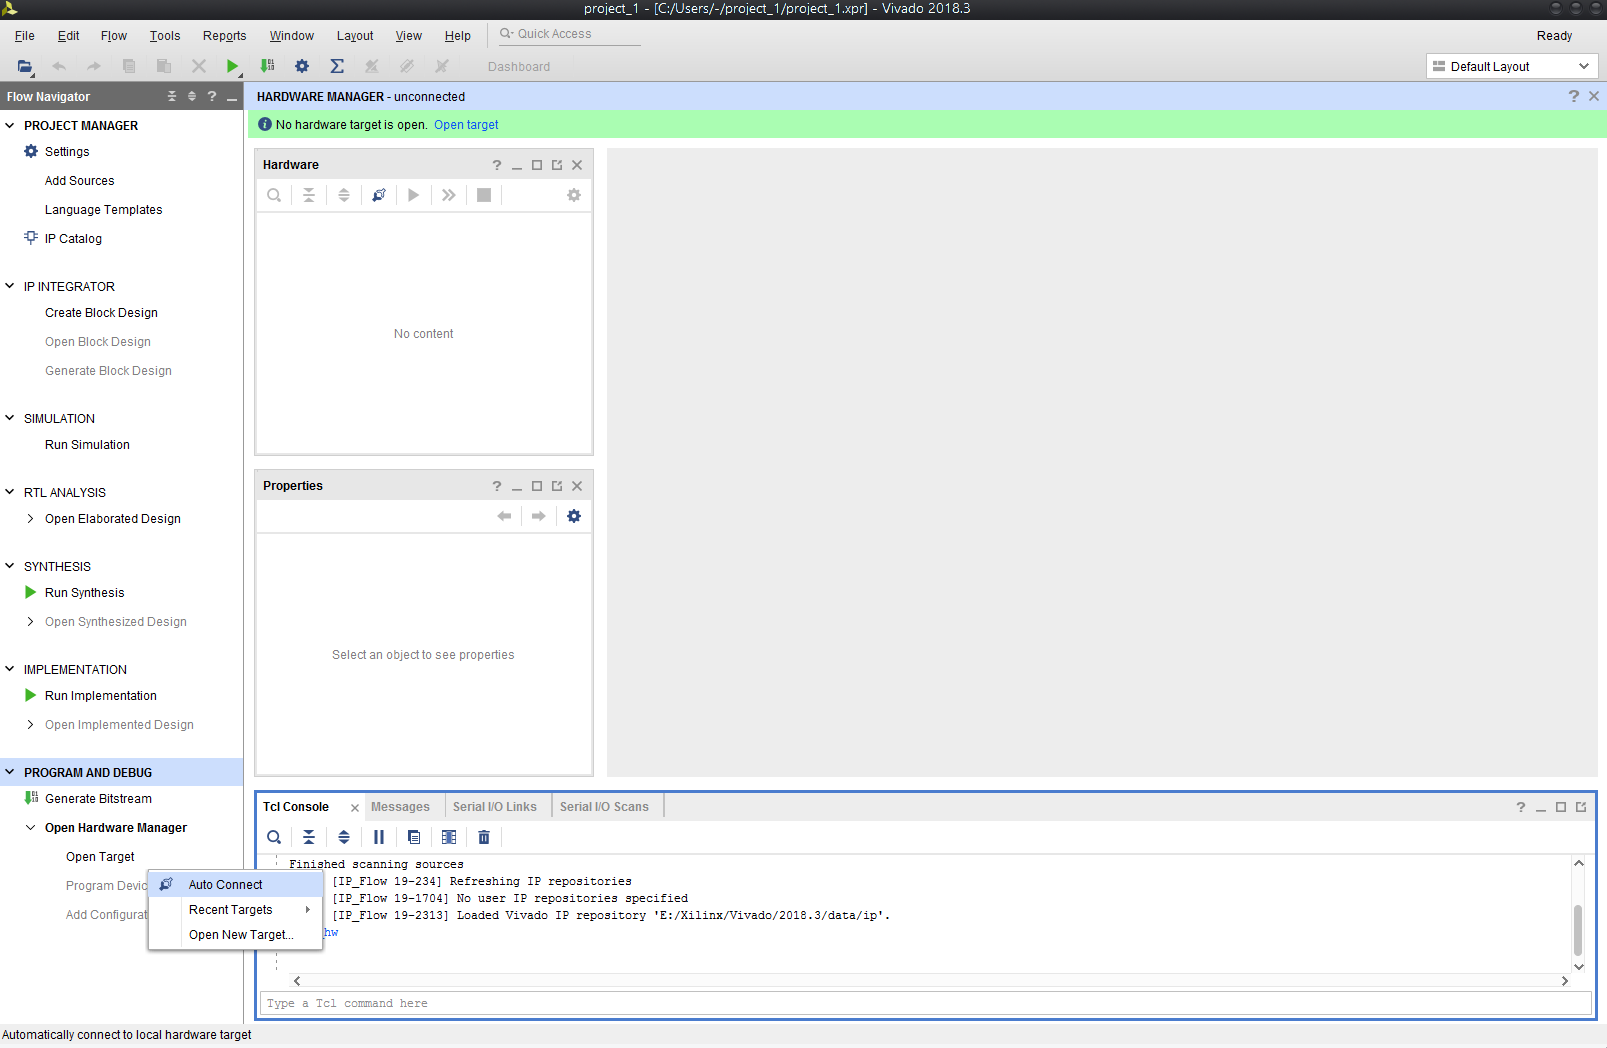
\includegraphics[width=\linewidth]{images/vivado03.png}
  \caption{Step 3: Connect to FPGA}
  \label{fig:vivado03}
\end{figure}

Under "Hardware Manager", choose "Open Target", then "Auto Connect".

\begin{figure}
  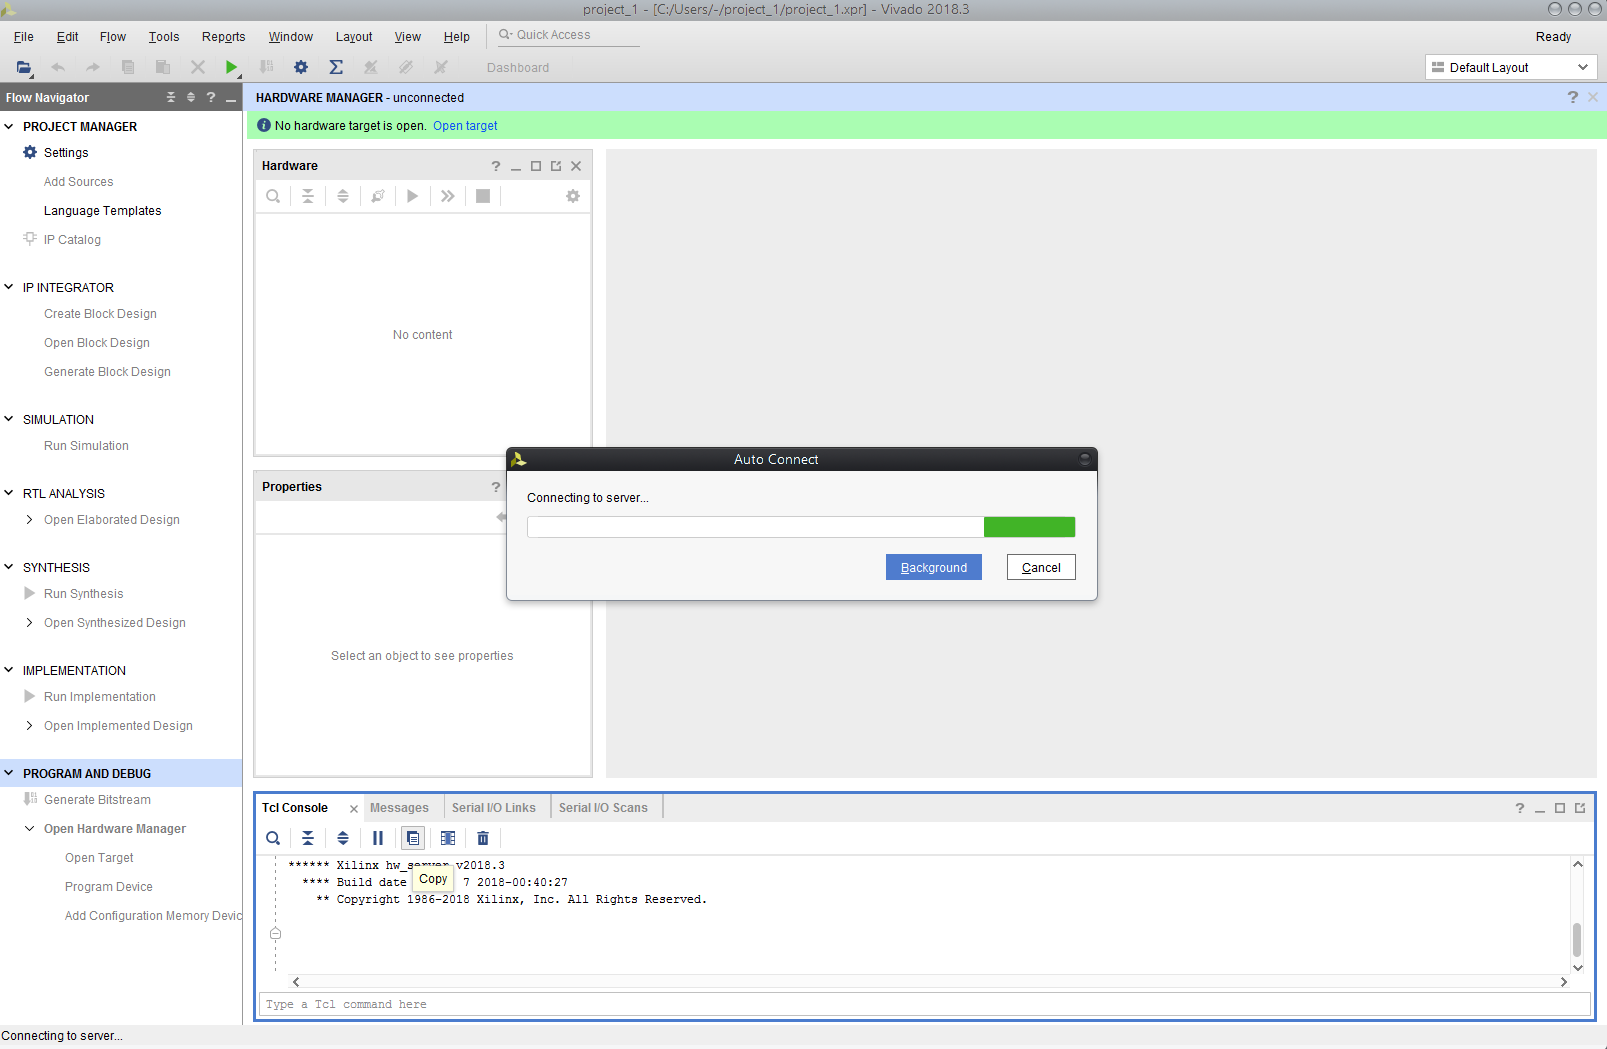
\includegraphics[width=\linewidth]{images/vivado04.png}
  \caption{Step 4: Wait a moment}
  \label{fig:vivado04}
\end{figure}

Wait a moment, "Connecting to server..."  should automatically close without dropping an error to the console.

\begin{figure}
  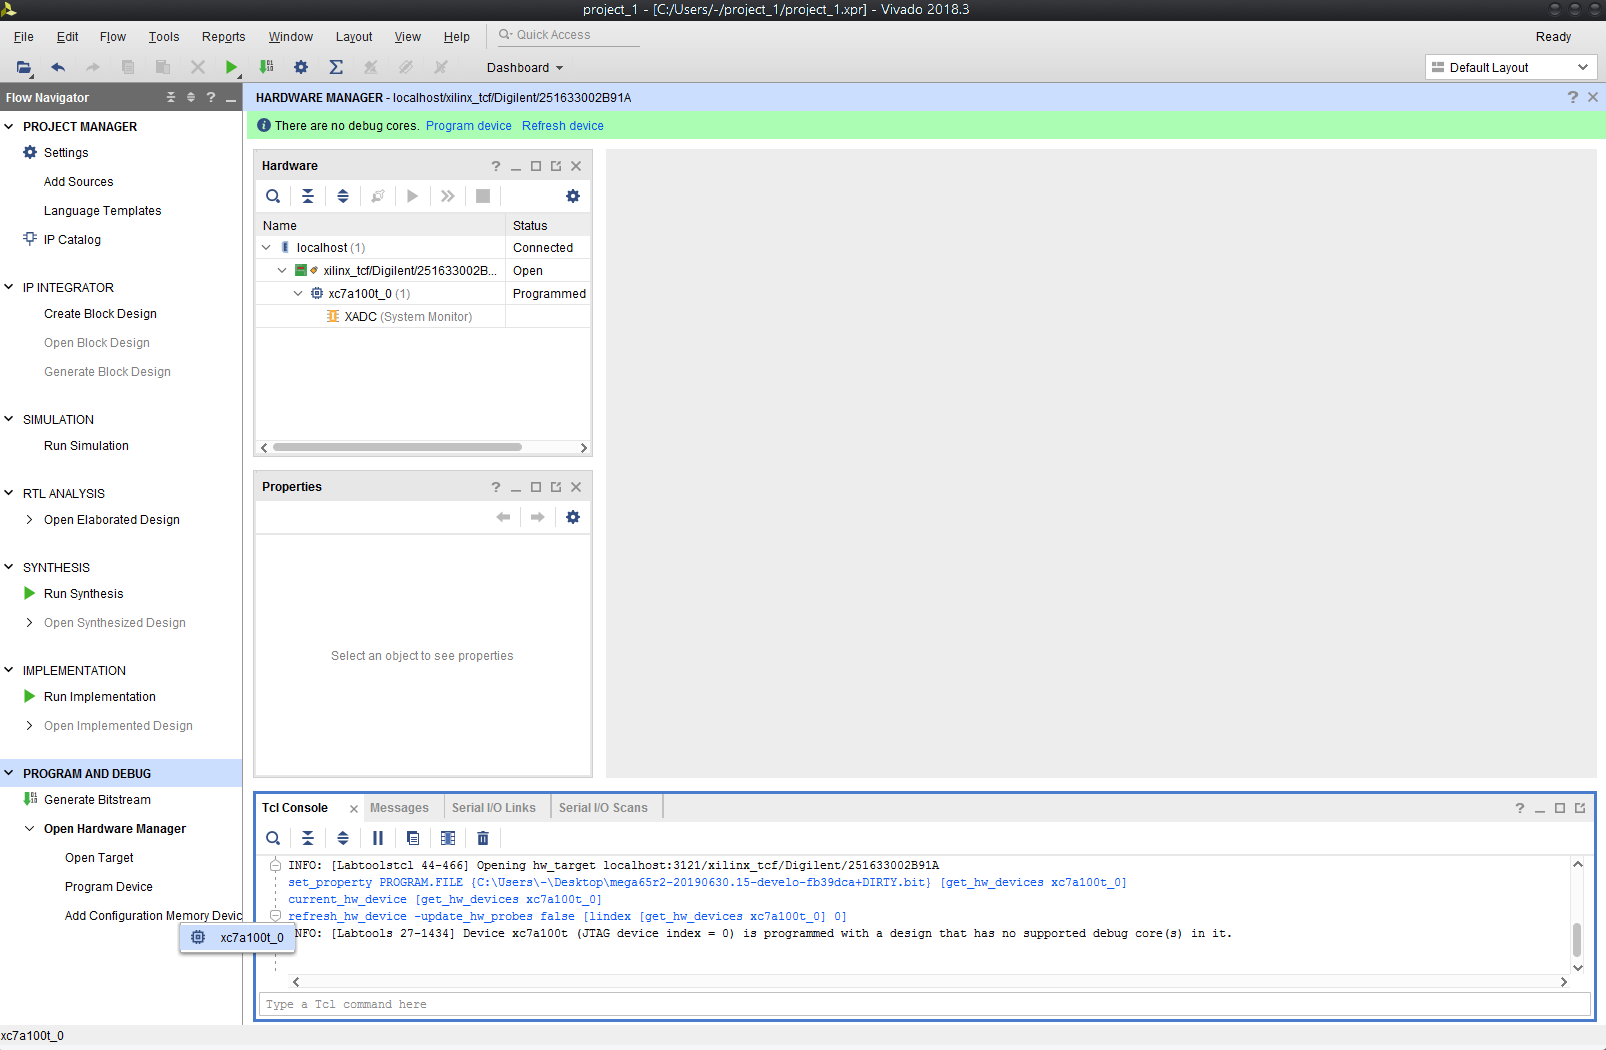
\includegraphics[width=\linewidth]{images/vivado05.png}
  \caption{Step 5: Add Configuration Memory Device}
  \label{fig:vivado05}
\end{figure}

Under "Hardware Manager", choose "Add Configuration Memory Device", then "xc7a100t\_0".

\begin{figure}
  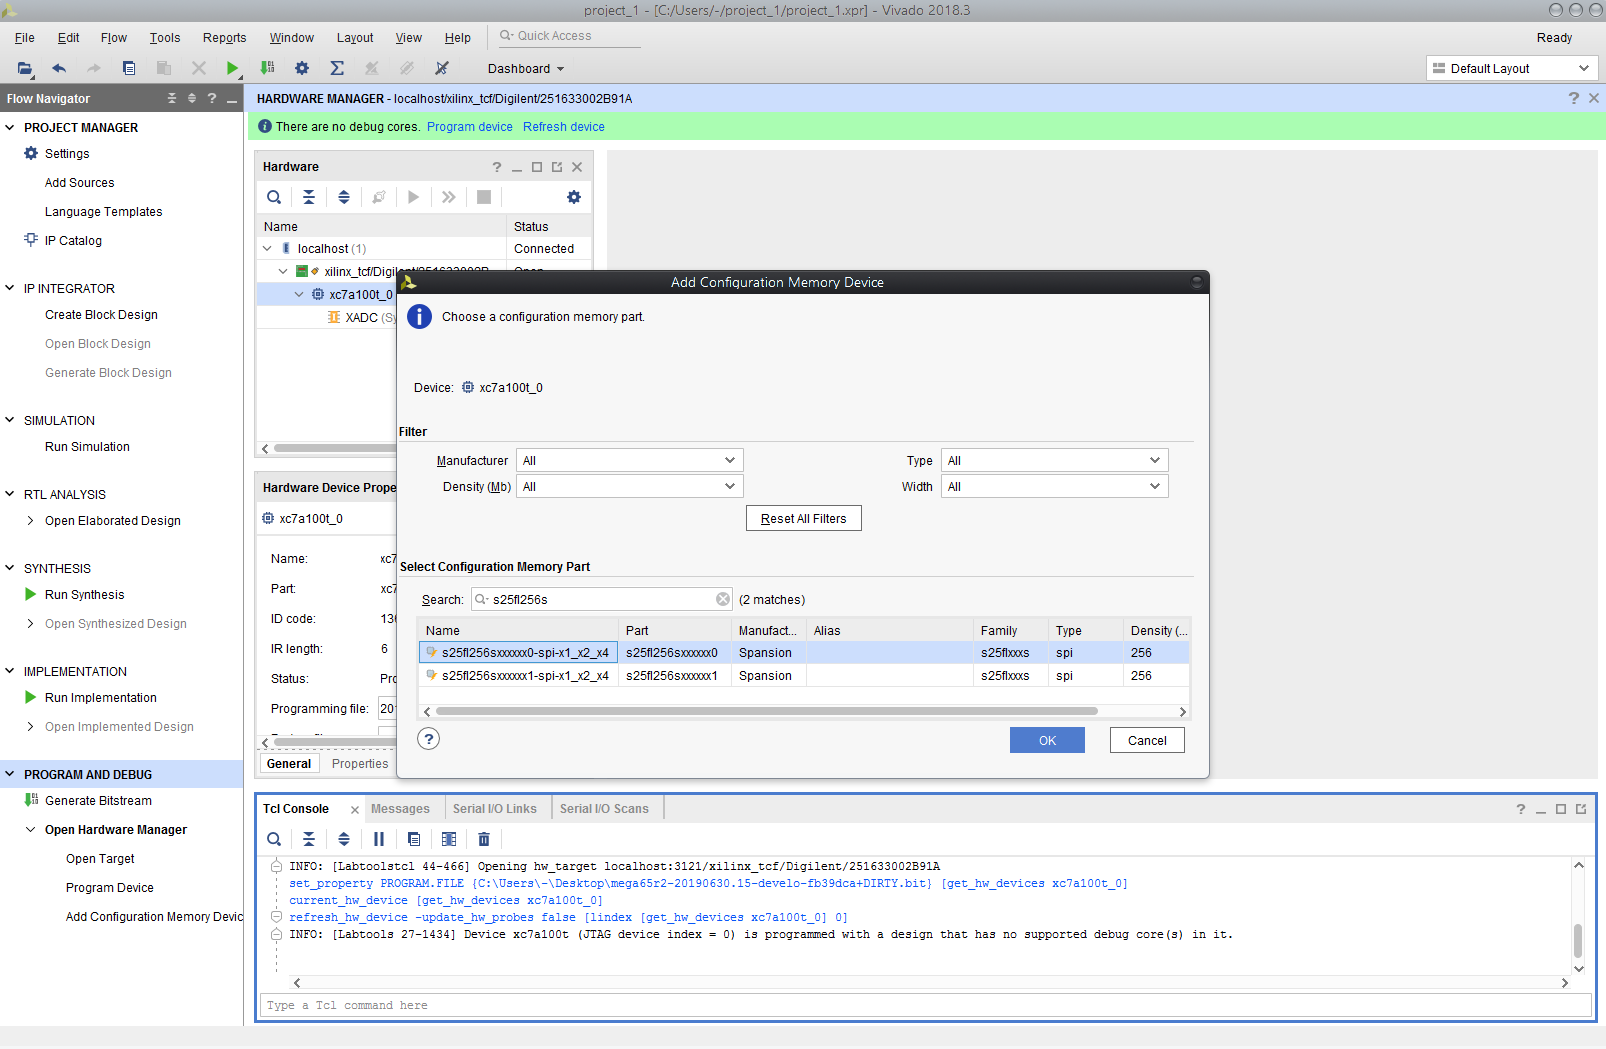
\includegraphics[width=\linewidth]{images/vivado06.png}
  \caption{Step 6: Select Memory Part}
  \label{fig:vivado06}
\end{figure}

In the newly opened dialogue, type "S25fl256s" (without quotes), then select "s25fl256sxxxxxxx0-spi-x1\_x2\_x4" (the upper one) and click "OK".

\begin{figure}
  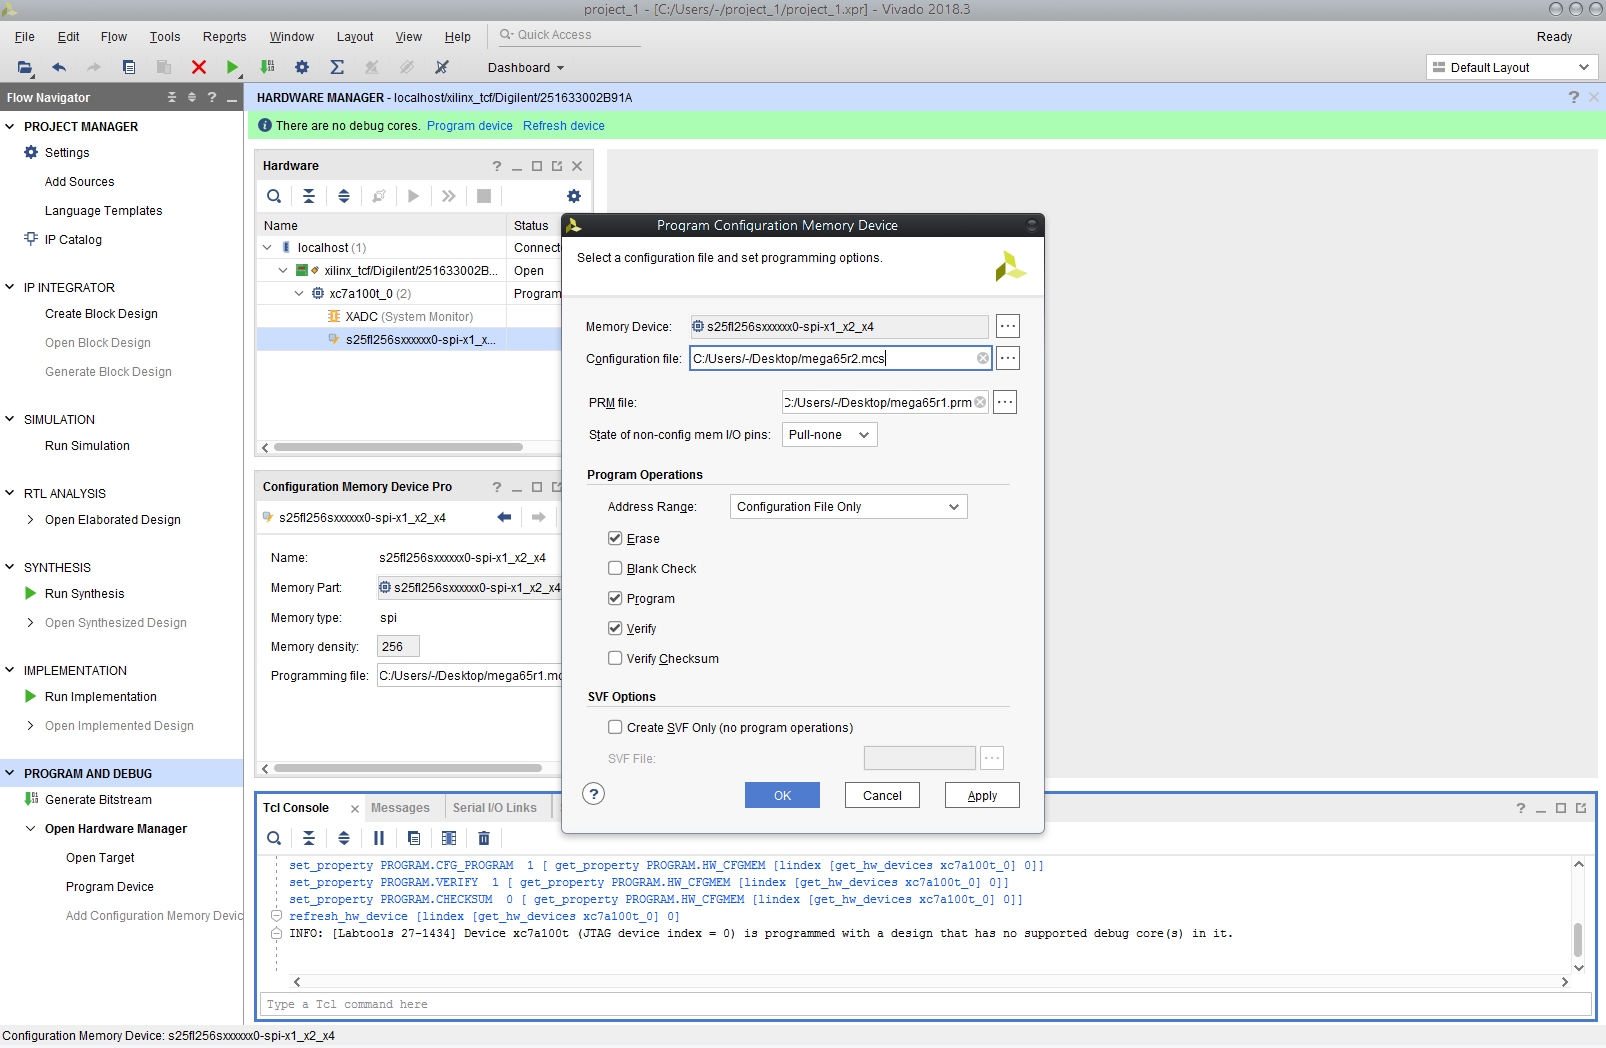
\includegraphics[width=\linewidth]{images/vivado07.png}
  \caption{Step 7: Set programming options}
  \label{fig:vivado07}
\end{figure}

In the next dialogue, choose your local Configuration file, namely a bitstream with file suffix ".mcs". Leave all other parameters as they are (see \ref{fig:vivado07}).

\begin{figure}
  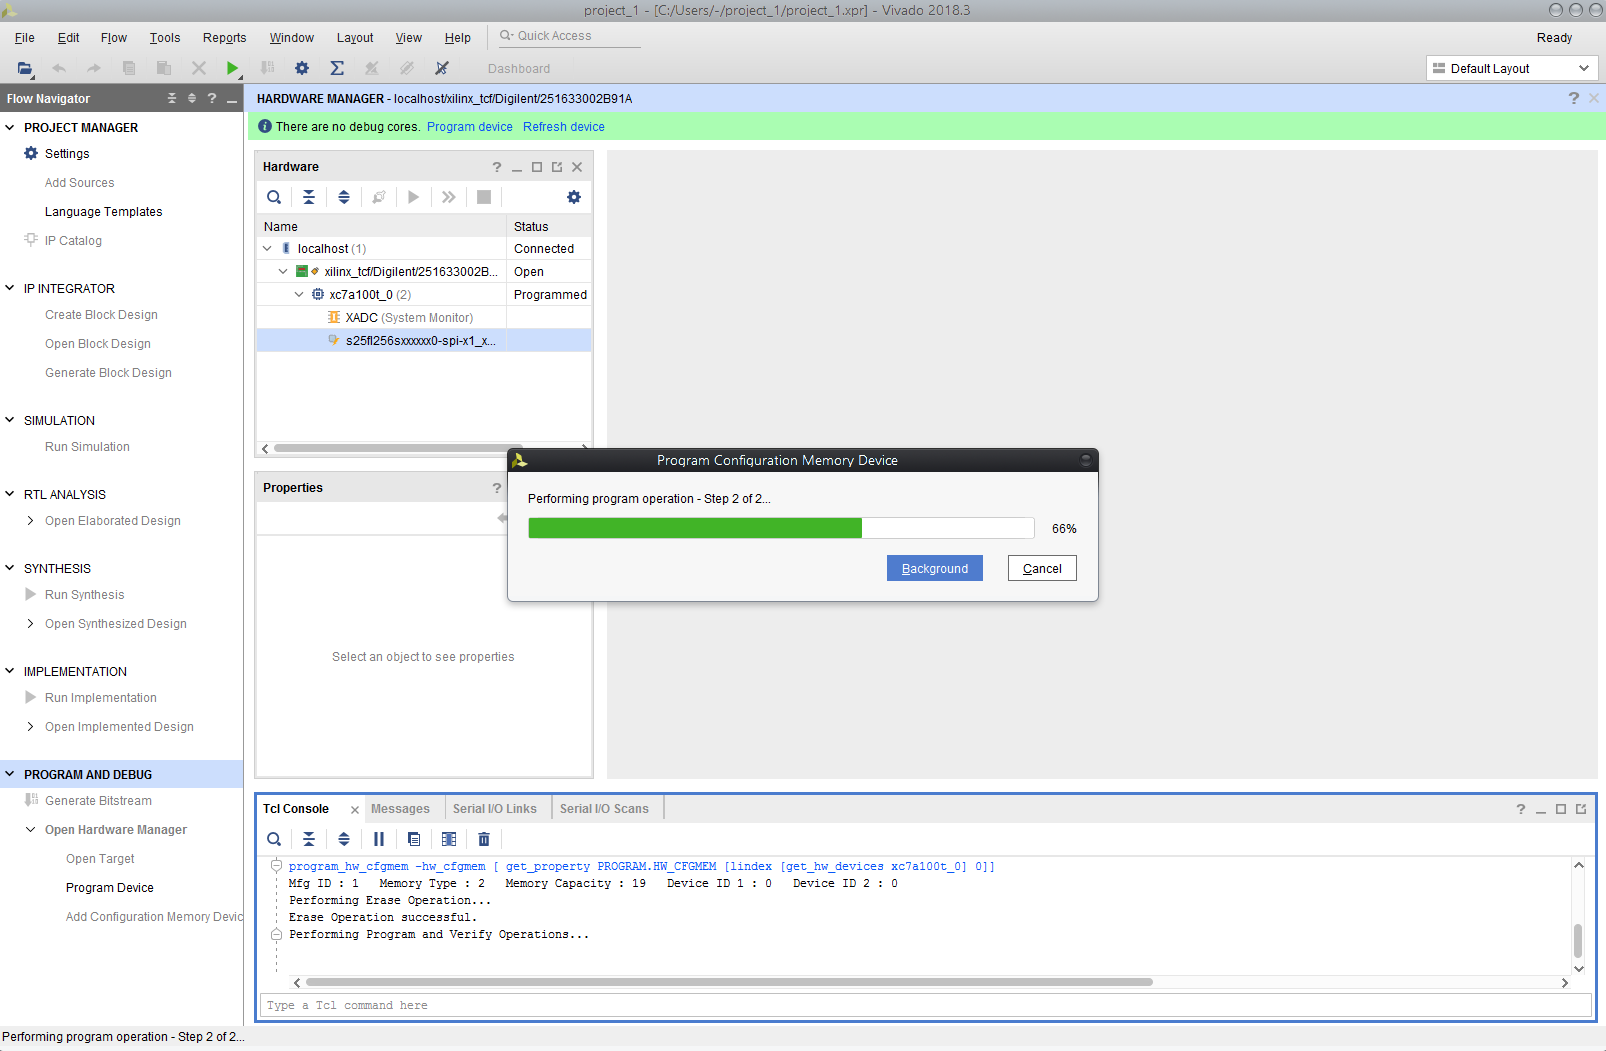
\includegraphics[width=\linewidth]{images/vivado08.png}
  \caption{Step 8: Programming in progress}
  \label{fig:vivado08}
\end{figure}

Patiently wait for the programming to finish. This can take several minutes as the Vivado software erases and then reprograms
the flash memory that is used to initialise the FPGA on power-up.

\begin{figure}
  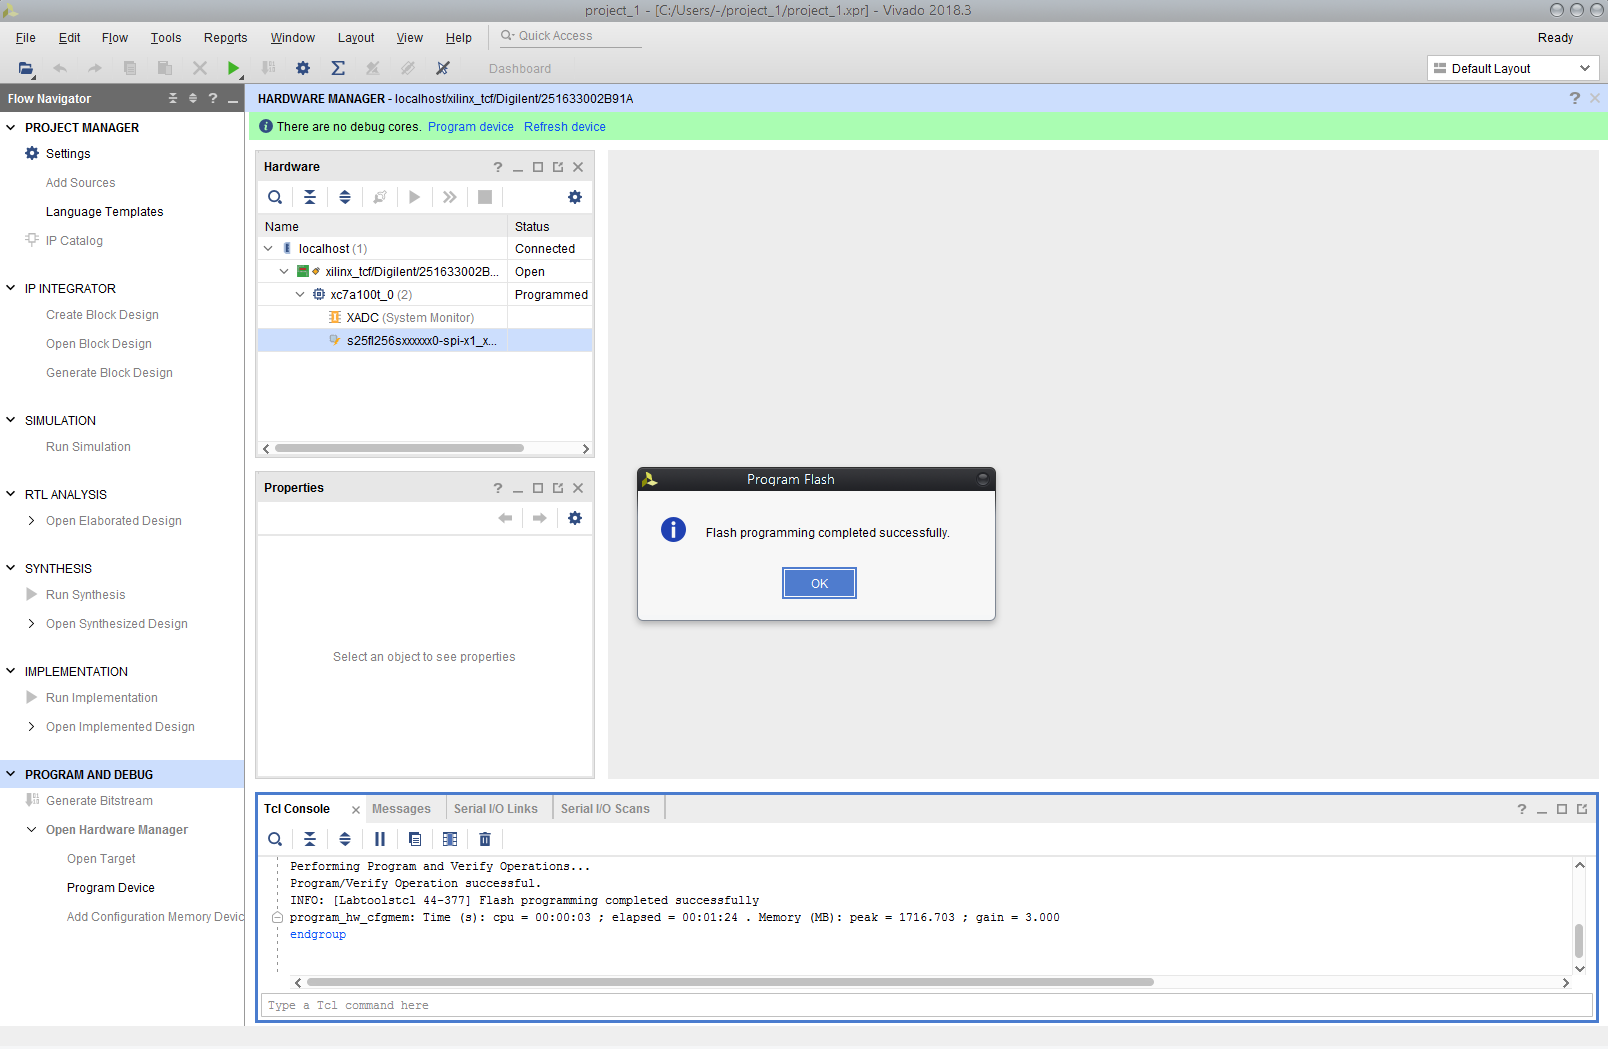
\includegraphics[width=\linewidth]{images/vivado09.png}
  \caption{Step 9: Programming successful}
  \label{fig:vivado09}
\end{figure}

If your screen looks like \ref{fig:vivado09}, your new bistream has been successfully flashed into the Artix 100T FPGA!

\begin{figure}
  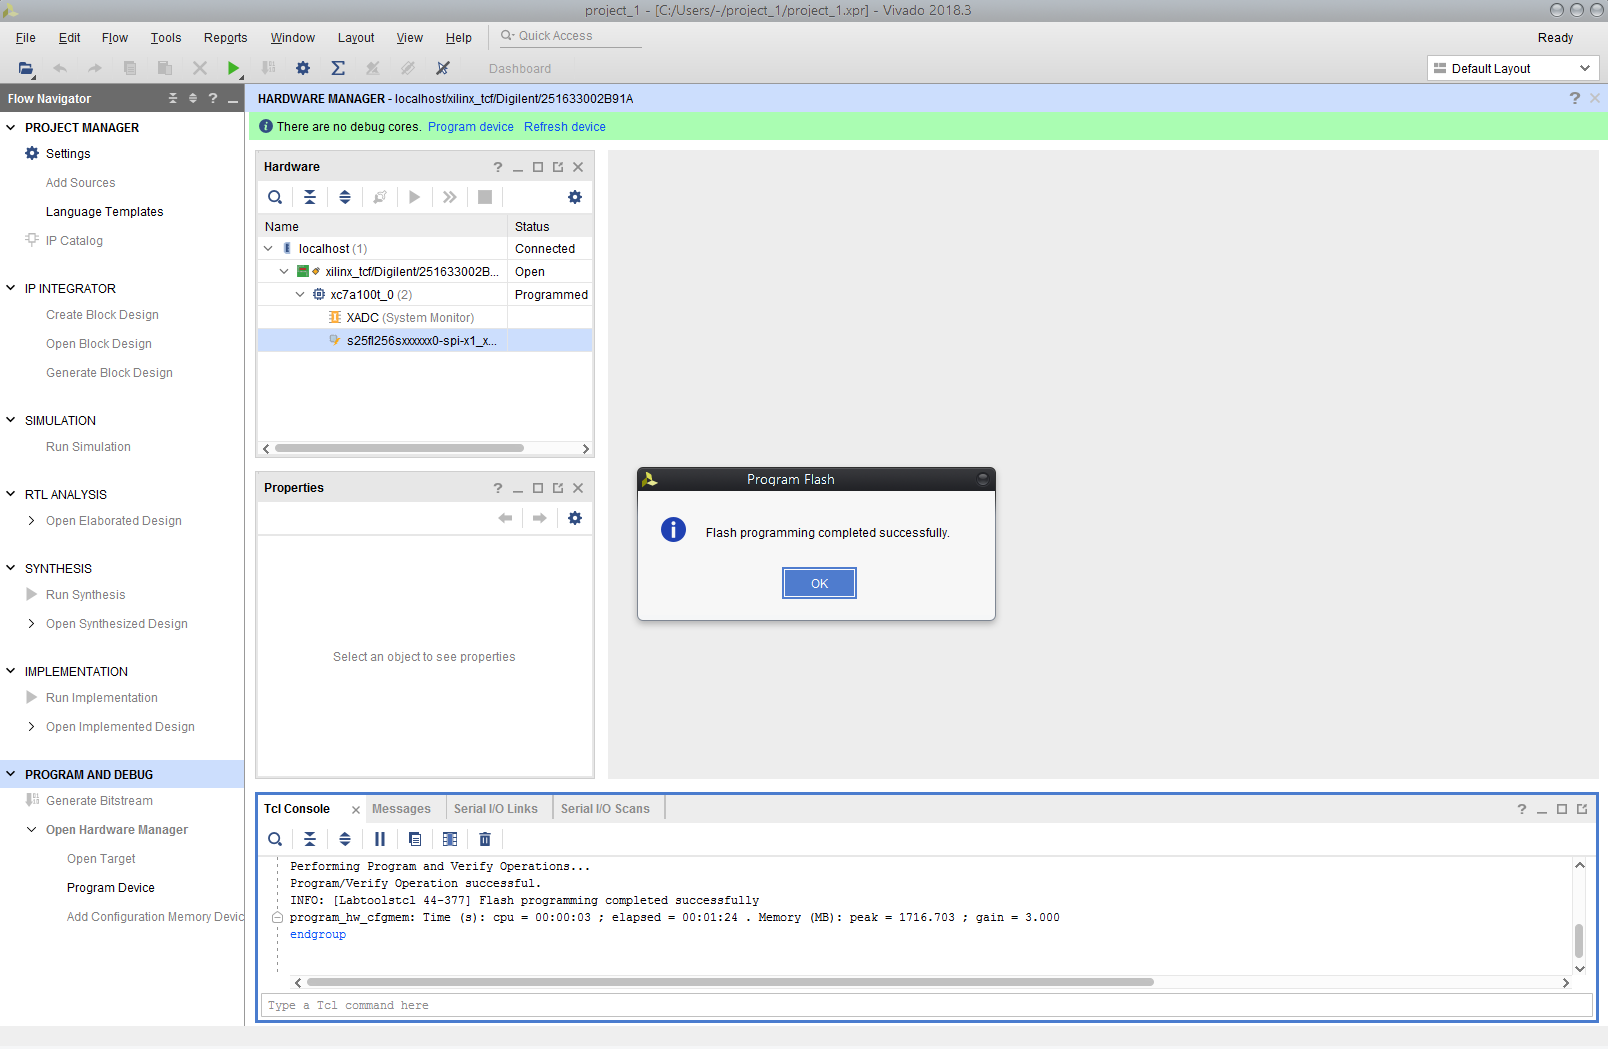
\includegraphics[width=\linewidth]{images/vivado09.png}
  \caption{Step 10: Reflashing the FPGA}
  \label{fig:vivado10}
\end{figure}

If you want to repeat the process, you might find the "Add Configuration Memory Device" option in step 5 greyed out. Instead, select "s25fl256sxxxxxxx0-spi-x1\_x2\_x4"  in the "Hardware" window, press right mouse button and select "Program Configuration Memory Device" to flash.

\section{Flashing the CPLD in the MEGA65's Keyboard with LATTICE DIAMOND}


If you choose to proceed, you will need a TE0790-03 JTAG programming module, a functioning
installation of Lattice Diamond Programmer software.  This can be done on either Windows or Linux, but
in both cases you will need to install any necessary USB drivers. It is also necessary to have
dip-switches 1 and 3 in the ON position and dip-switches 2 and 4 in the OFF position on the TE-0790.
With your MEGA65 disconnected from the power, the TE-0790 must be installed on the JB1 connector,
which is located between the floppy data cable and the audio jack.
The gold-plated hole of the TE-0790 must line up with the screw
hole below.  The mini-USB cable will then connect on the side towards the 3.5" floppy drive.
The following image shows the correct position: The TE0790 is surrounded by the yellow box,
and the dip-switches by the red box. Dip-switch 1 is the one nearest the floppy data cable.


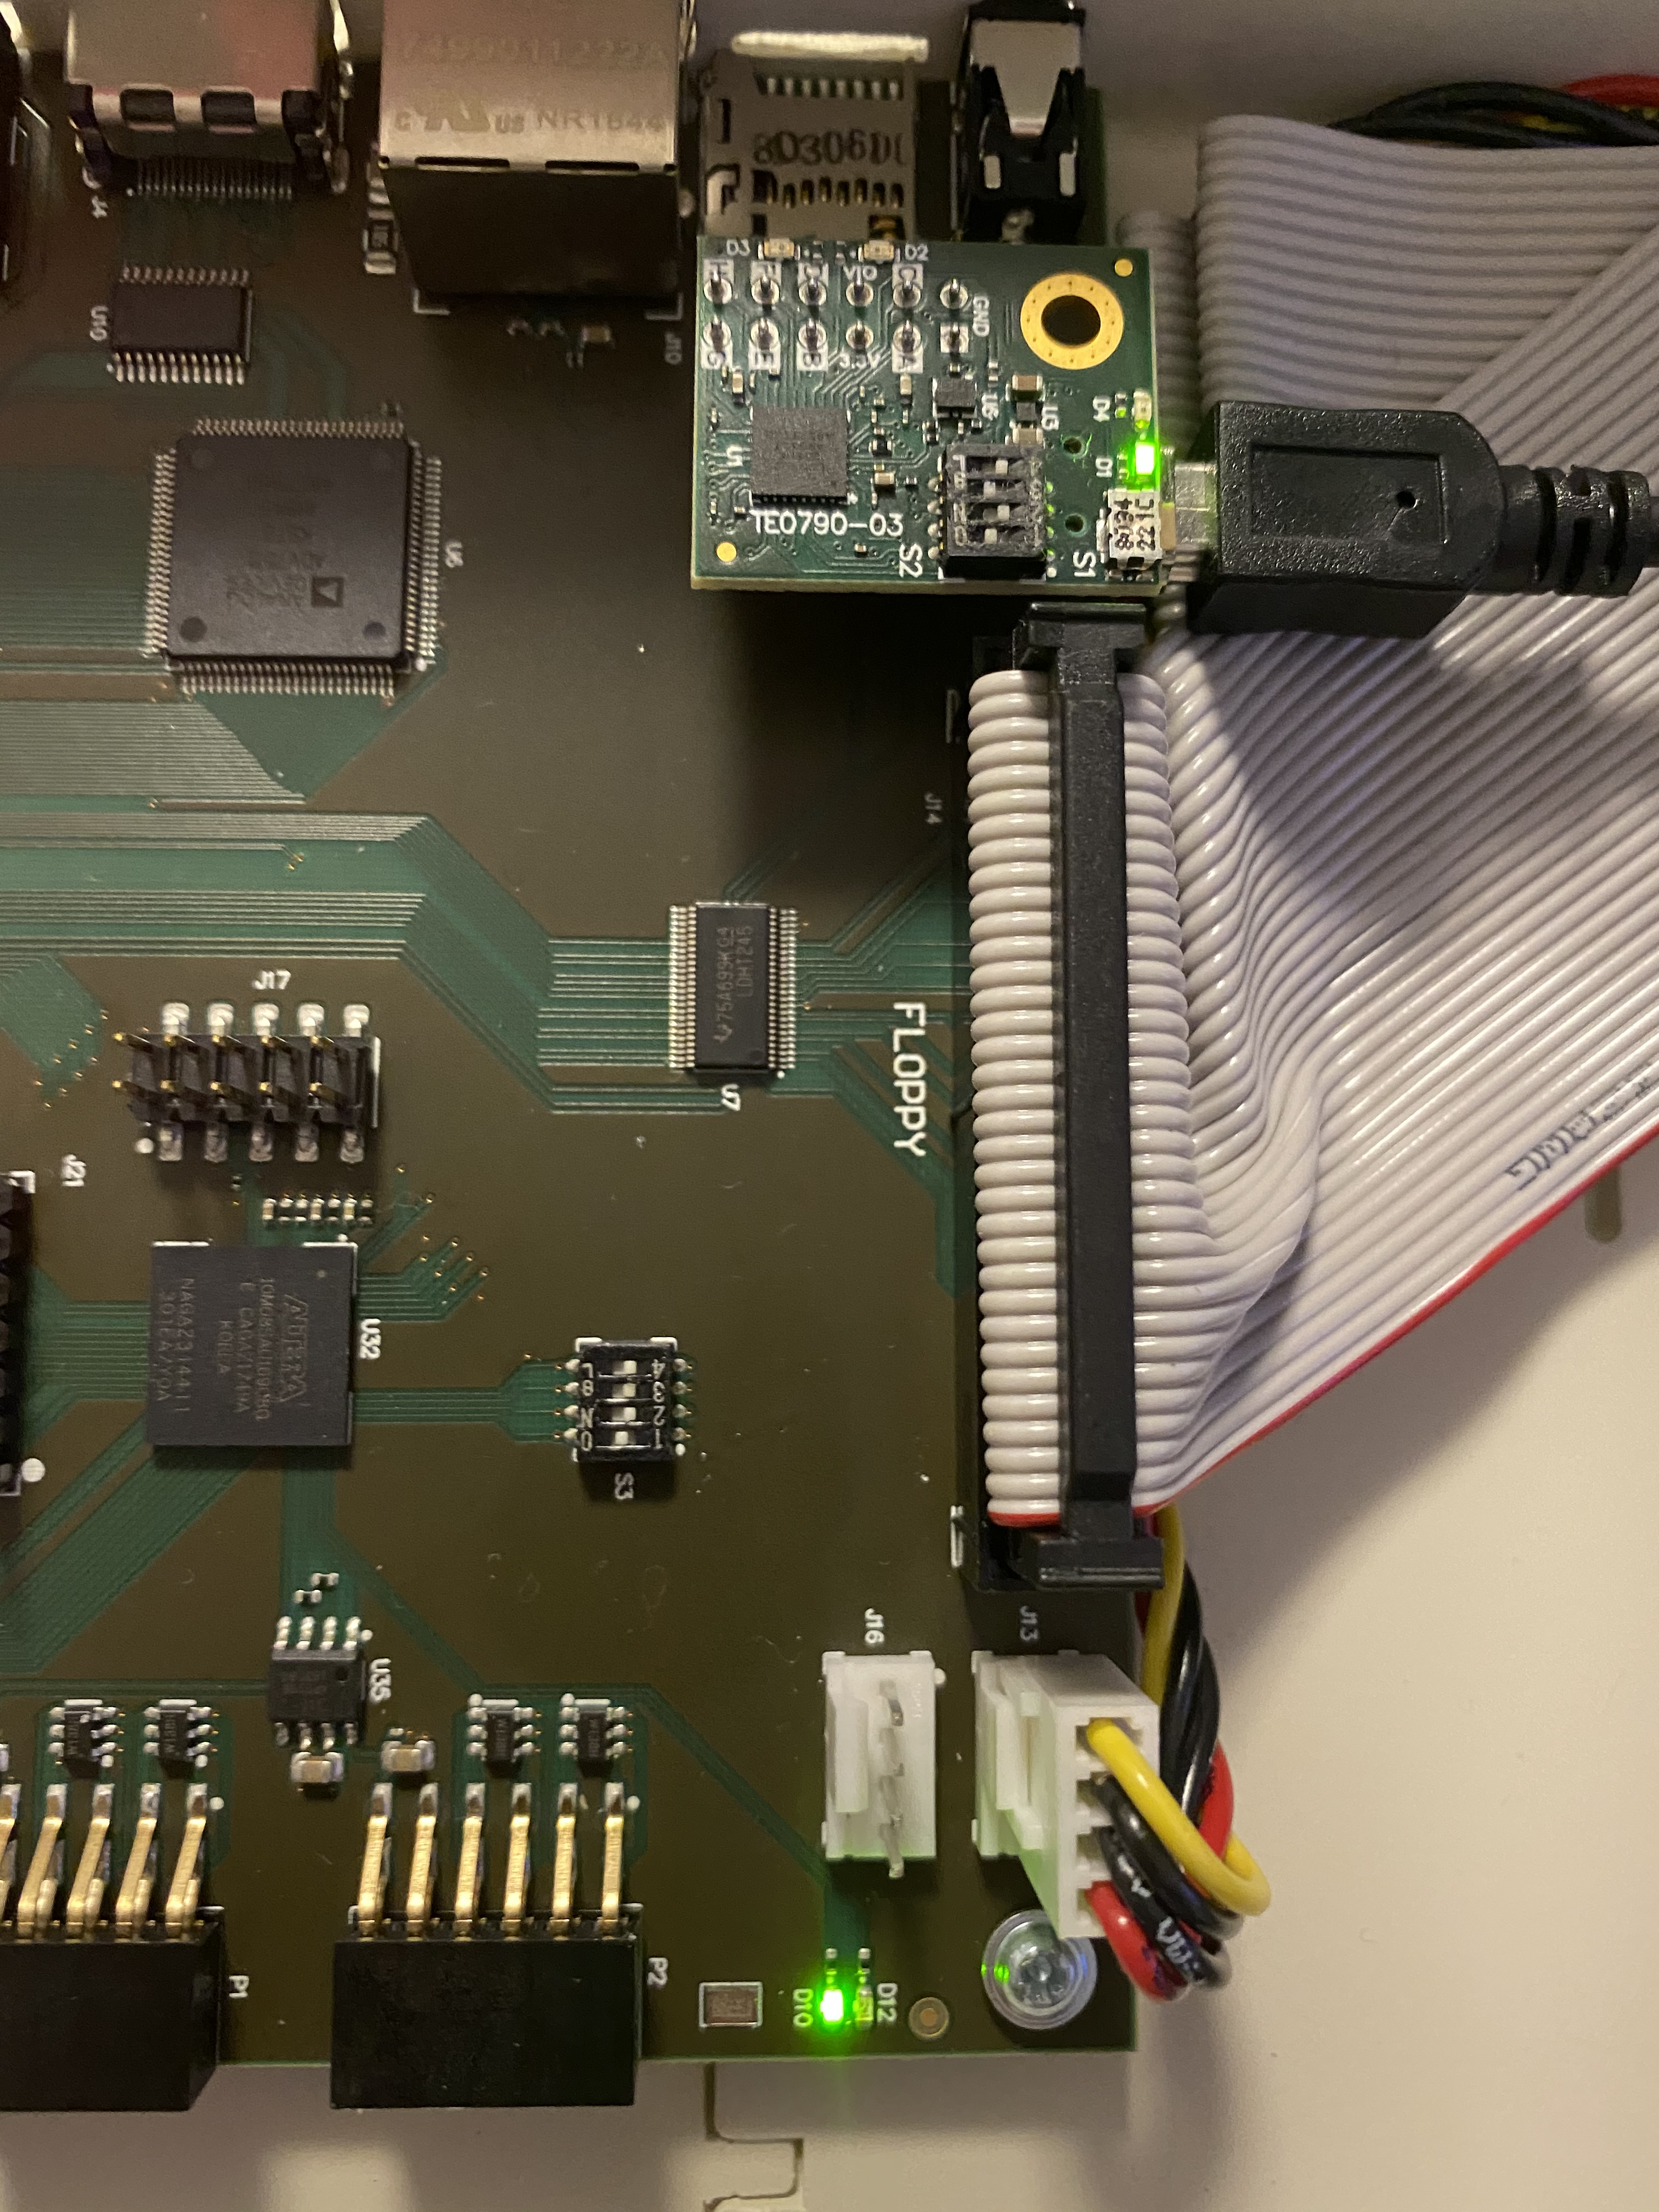
\includegraphics[width=\linewidth]{images/jtag_detail_05.jpg}


One the PCB r2 MEGA65 Mainbord dip switch 1 (the one nearest to the user sitting in front of the machine
must be in the ON position, the other switches must be OFF. The keyboard will go into "Police Mode"
(blue and red blinking LEDs) when set correctly.

Connect your non-8-bit computer to the FPGA programming device using a mini-USB cable. Switch
the MEGA65 computer ON. Open DIAMOND PROGRAMMER, which can be downloaded from the internets.

\begin{figure}
  
\includegraphics{images/diamond01.png}
  \caption{Step 1: Open DIAMOND PROGRAMMER}
  \label{fig:diamond01}
\end{figure}

Select "Create a new project from a JTAG scan". If entry under "Cable:" is empty, click "Detect Cable".

\begin{figure}
  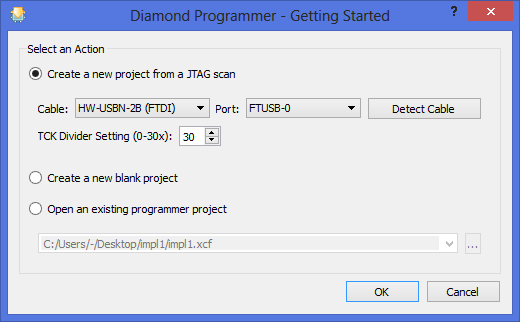
\includegraphics[width=\linewidth]{images/diamond02.png}
  \caption{Step 2: Create a new project}
  \label{fig:diamond02}
\end{figure}

If dialog "Programmer: Multiple Cables Detected" appears, select the first entry ("Location 0000") and click "OK".

\begin{figure}
  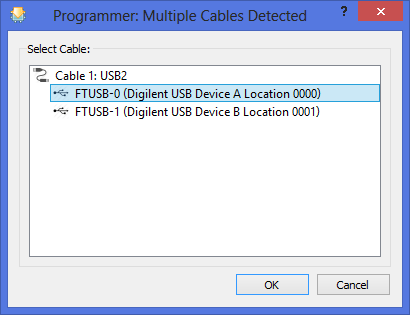
\includegraphics[width=\linewidth]{images/diamond03.png}
  \caption{Step 3: Select cable}
  \label{fig:diamond03}
\end{figure}

You have now created a new project which should display "MachXO2" under "Device Family" and "LCMXO2-1200HC" under "Device"

\begin{figure}
  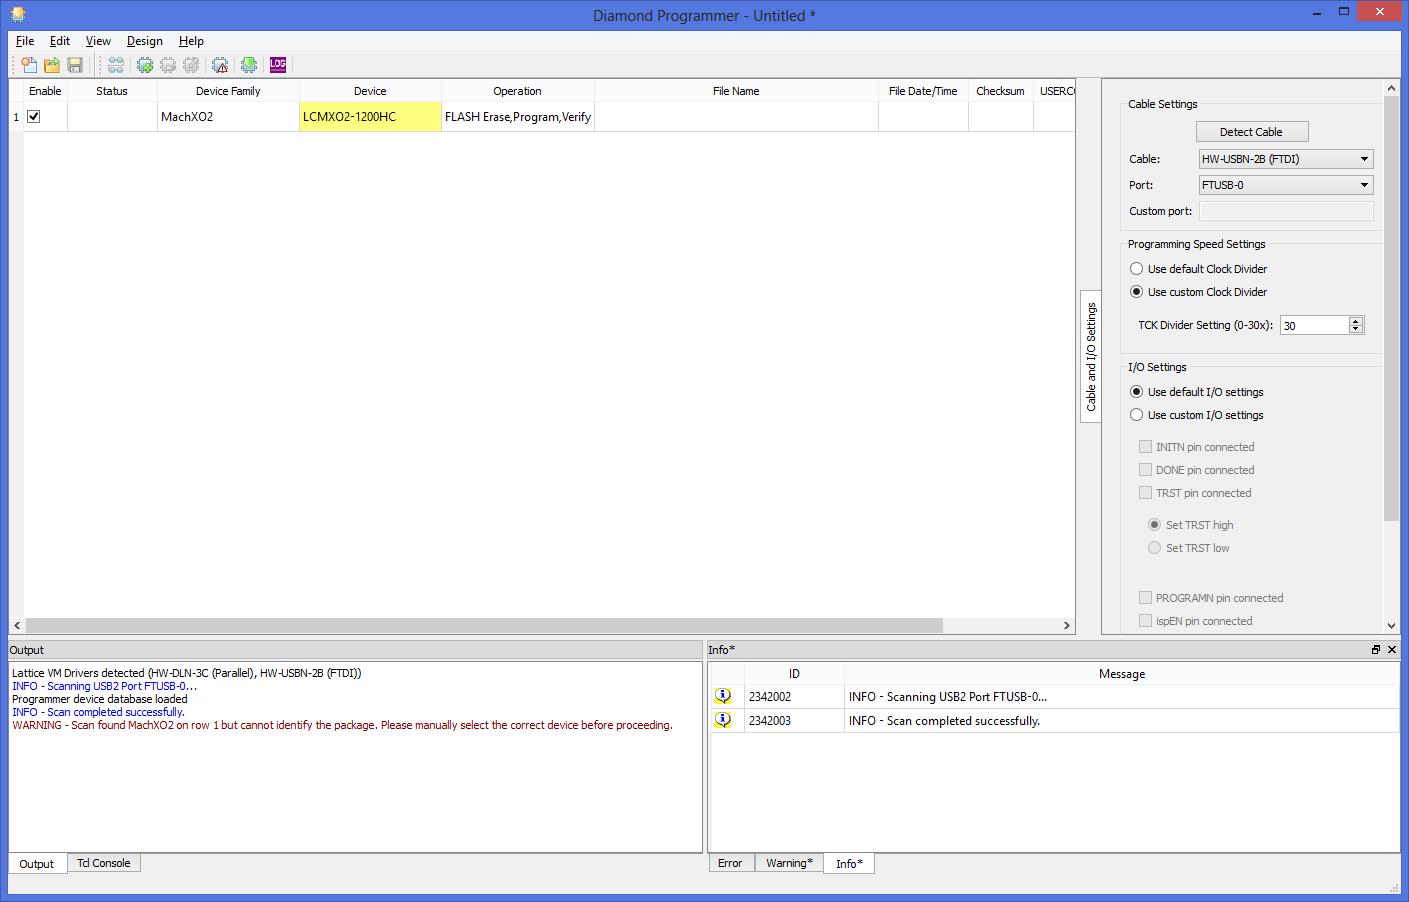
\includegraphics[width=\linewidth]{images/diamond04.png}
  \caption{Step 4: New Diamond Programmer project}
  \label{fig:diamond04}
\end{figure}

Choose "File"  then "Open File" to load the DIAMOND PROGRAMMER project with the MEGA65 keyboard firmware update.

\begin{figure}
  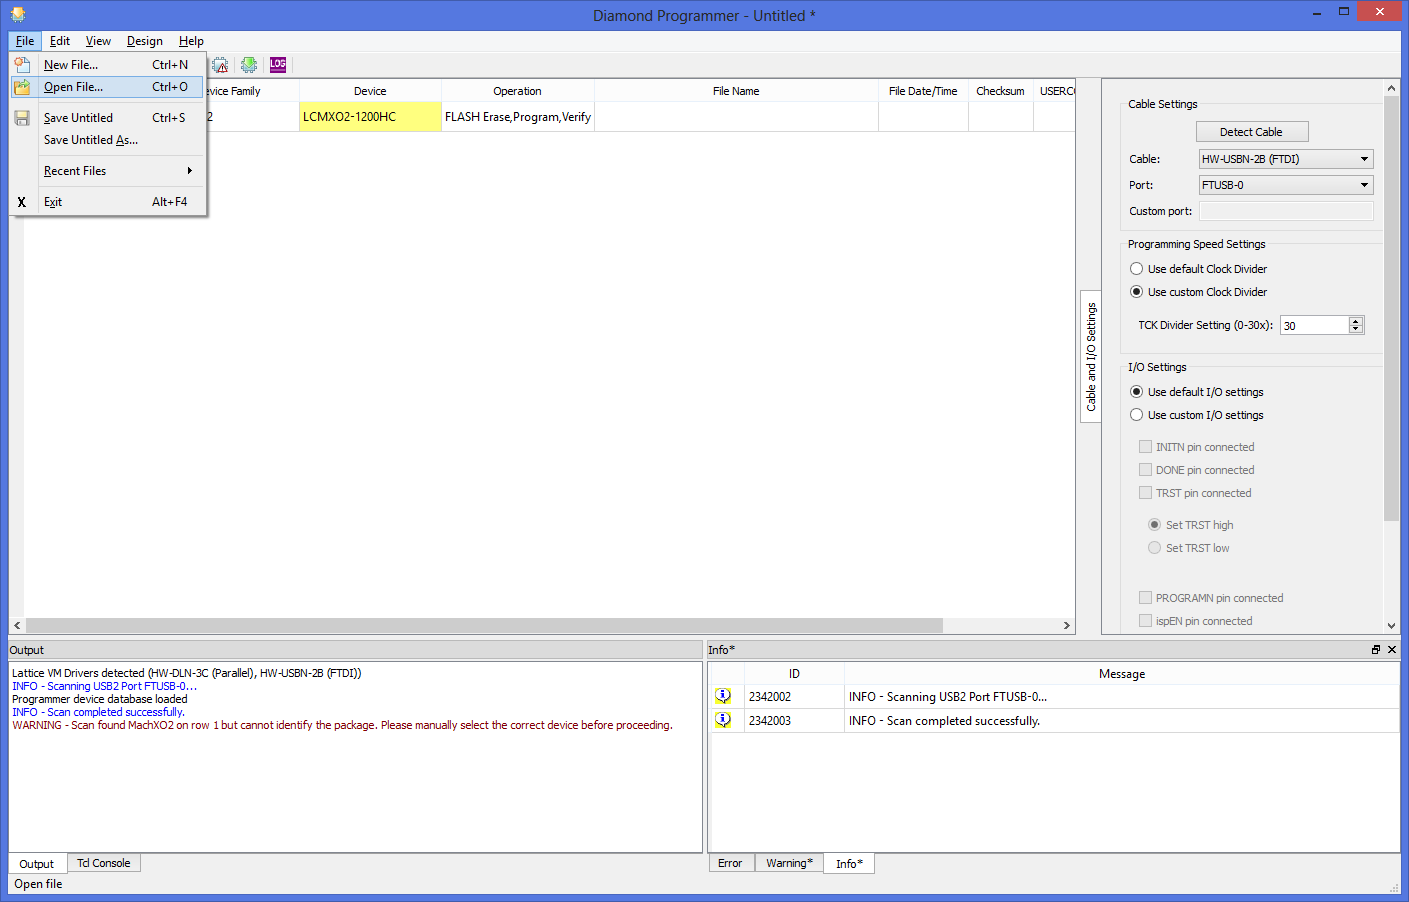
\includegraphics[width=\linewidth]{images/diamond05.png}
  \caption{Step 5: Open project}
  \label{fig:diamond05}
\end{figure}

Navigate into the folder with the extracted MEGA65 keyboard firmware files you have received and select the file ending with ".xcf".

\begin{figure}
  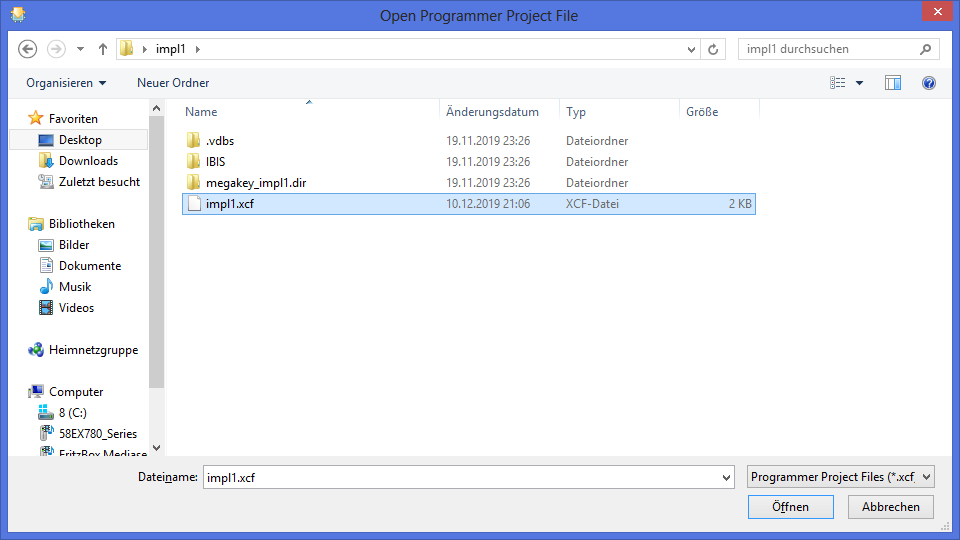
\includegraphics[width=\linewidth]{images/diamond06.png}
  \caption{Step 6: Select project file}
  \label{fig:diamond06}
\end{figure}

Click the three dots under "File Name" to set the correct path and find the file ending with ".jed".

\begin{figure}
  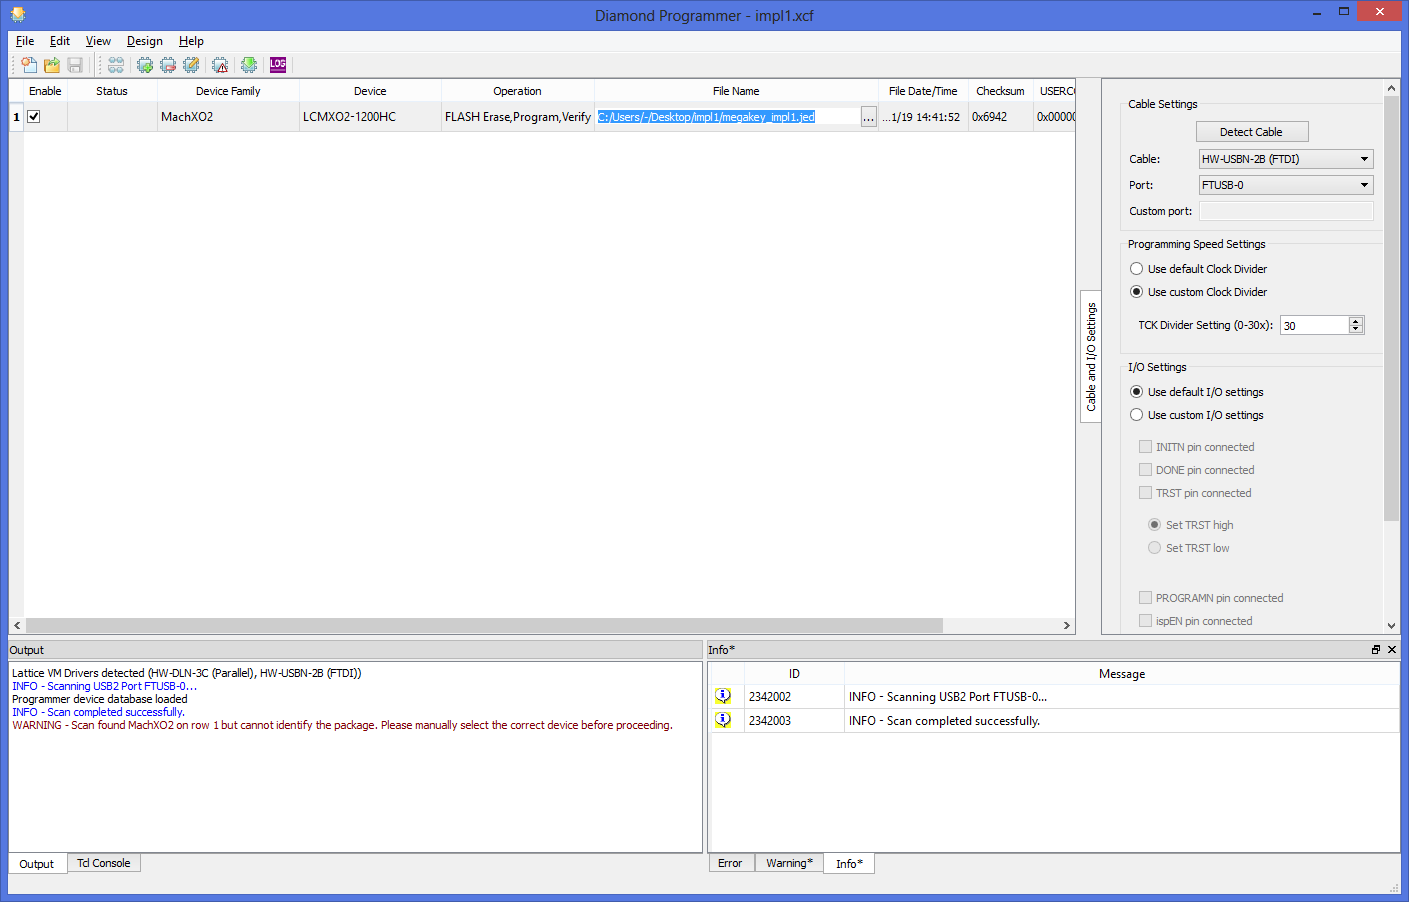
\includegraphics[width=\linewidth]{images/diamond07.png}
  \caption{Step 7: Choose correct path of .jed file}
  \label{fig:diamond07}
\end{figure}

Select the file ending with ".jed" and click "OK".

\begin{figure}
  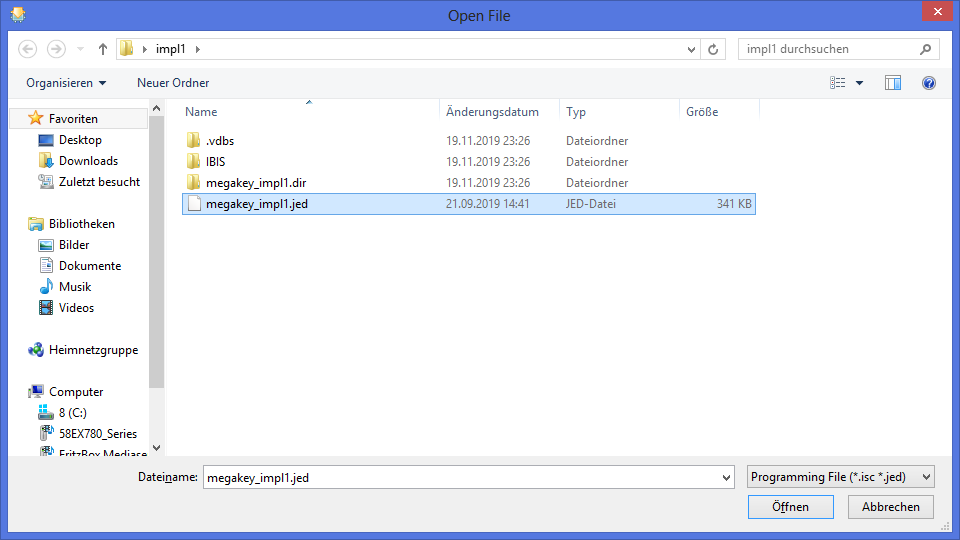
\includegraphics[width=\linewidth]{images/diamond08.png}
  \caption{Step 8: Select .jed file}
  \label{fig:diamond08}
\end{figure}

Click on the icon with the green arrow facing down "PROGRAM", which looks similar to the DIAMOND PROGRAMMER program icon.

\begin{figure}
  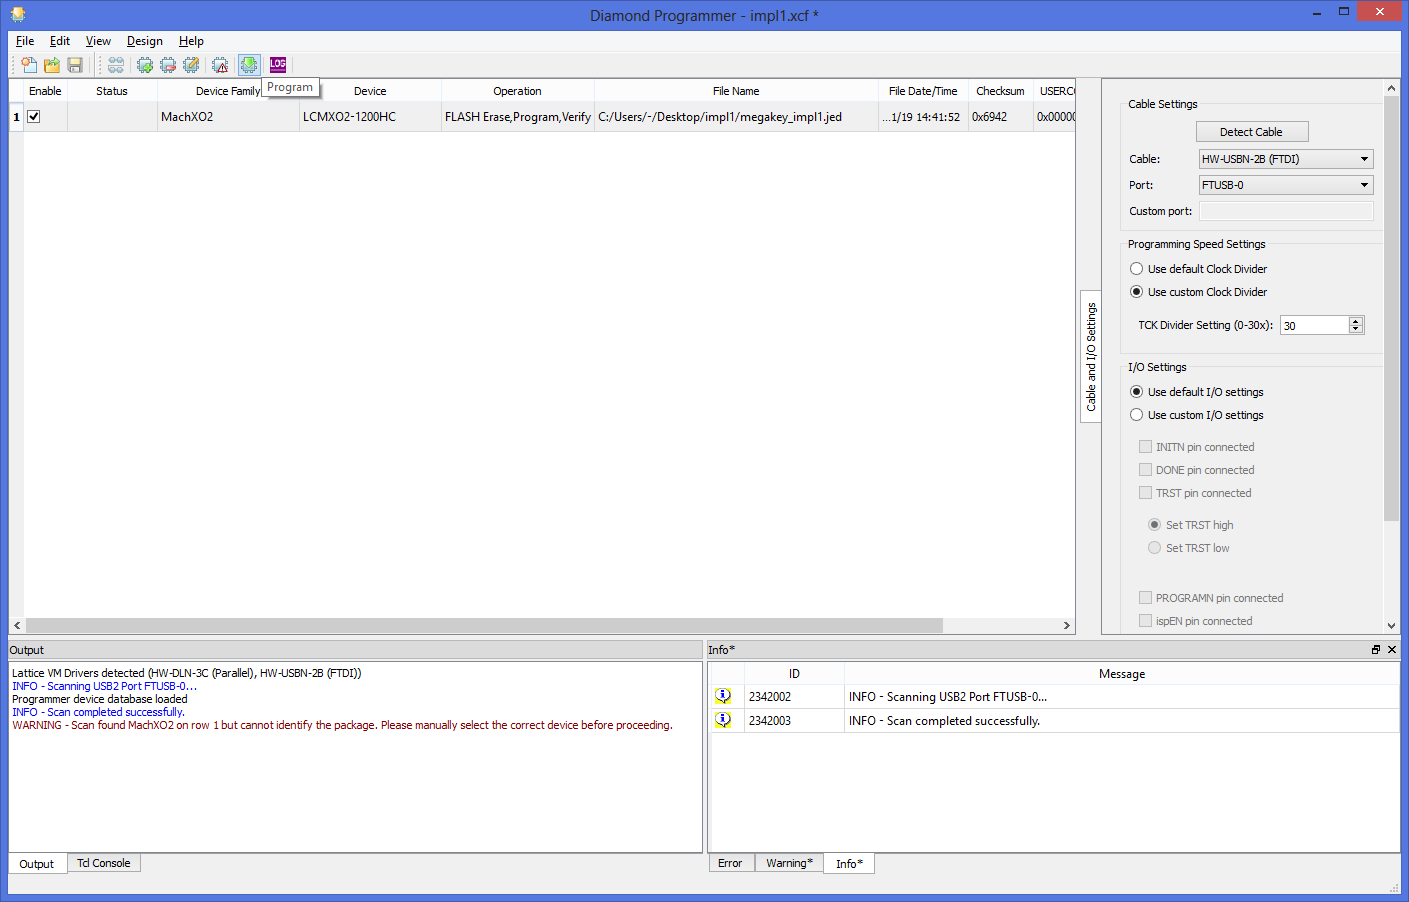
\includegraphics[width=\linewidth]{images/diamond09.png}
  \caption{Step 9: Select cable}
  \label{fig:diamond09}
\end{figure}

After a moment  the Output window should display "INFO - Operation: successful." and the "Status" cell should go green (does not always happen).

\begin{figure}
  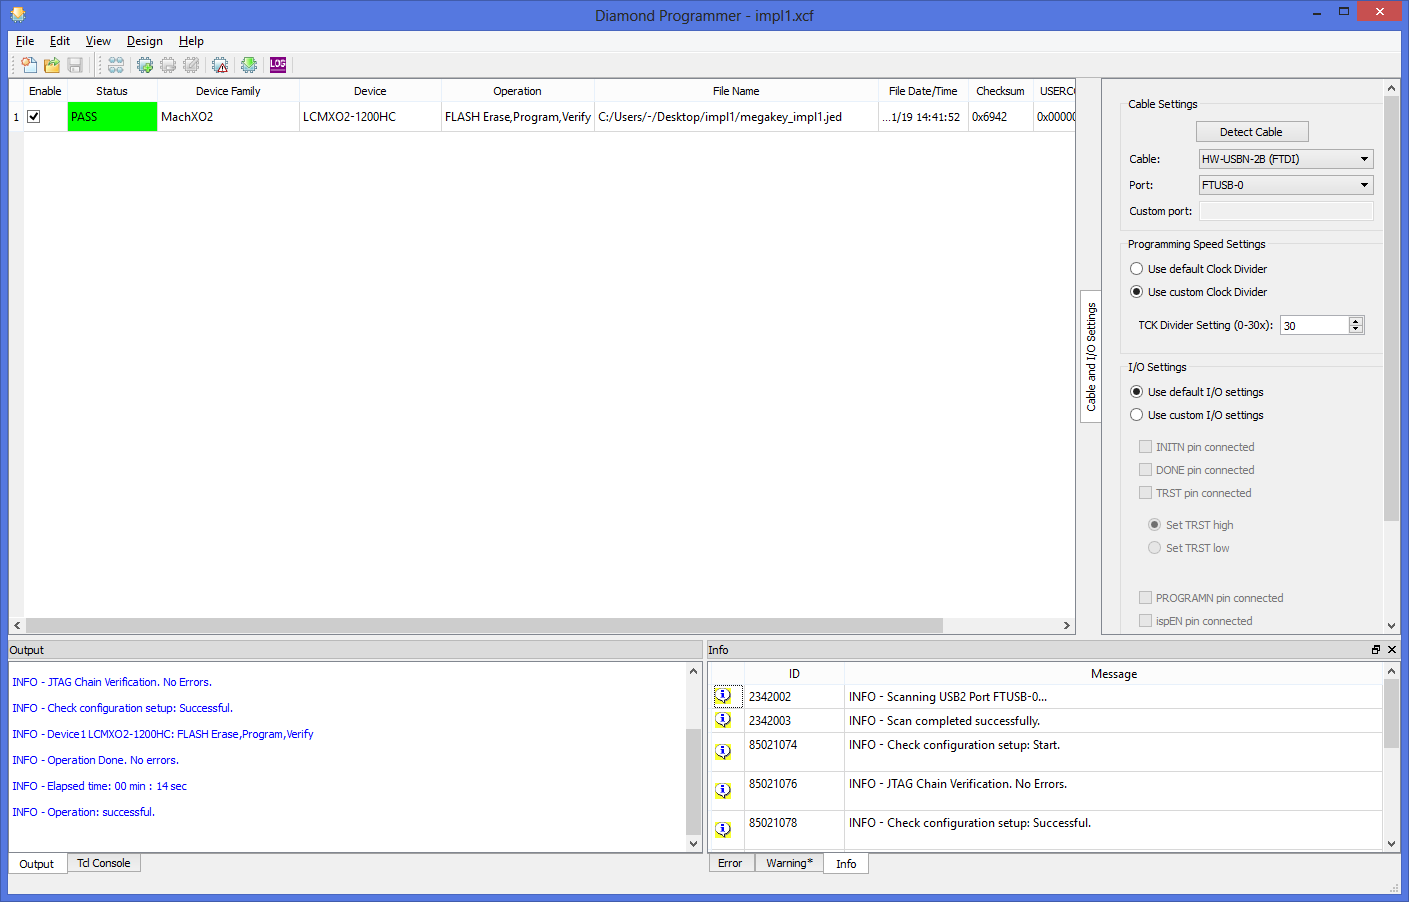
\includegraphics[width=\linewidth]{images/diamond10.png}
  \caption{Step 10: Operation successful}
  \label{fig:diamond10}
\end{figure}

You have now successfully flashed the MEGA65 keyboard. If you wish you can save the project now for later use.

\section{Flashing the MAX10 FPGA on the MEGA65's Mainboard with INTEL QUARTUS}

If you choose to proceed, you will need a TEI0004 - Arrow USB Programmer2 module with TEI0004 driver installed
and a functioning installation of Quartus Prime Programmer Lite Edition.  This can be done on either Windows
or Linux, but in both cases you will need to install any necessary USB drivers.
With your MEGA65 disconnected from the power, the TEI0004 must be installed on the J17 connector,
which is located between the floppy data cable and the ARTIX 7 FPGA on the Mainboard.
The micro-USB port of the TEI0004 must face in the opposite direction of the HDMI and LAN sockets, towards
the trap door.
The following image shows the correct position.

One the PCB r2 MEGA65 Mainbord all dip switches must be in the OFF. The Artix 100T main FPGA must not contain
a valid bitstream. See section "Flashing the Artix 100T main FPGA with XILINX VIVADO" on how to erase bitstream
from ARTIX 100T.

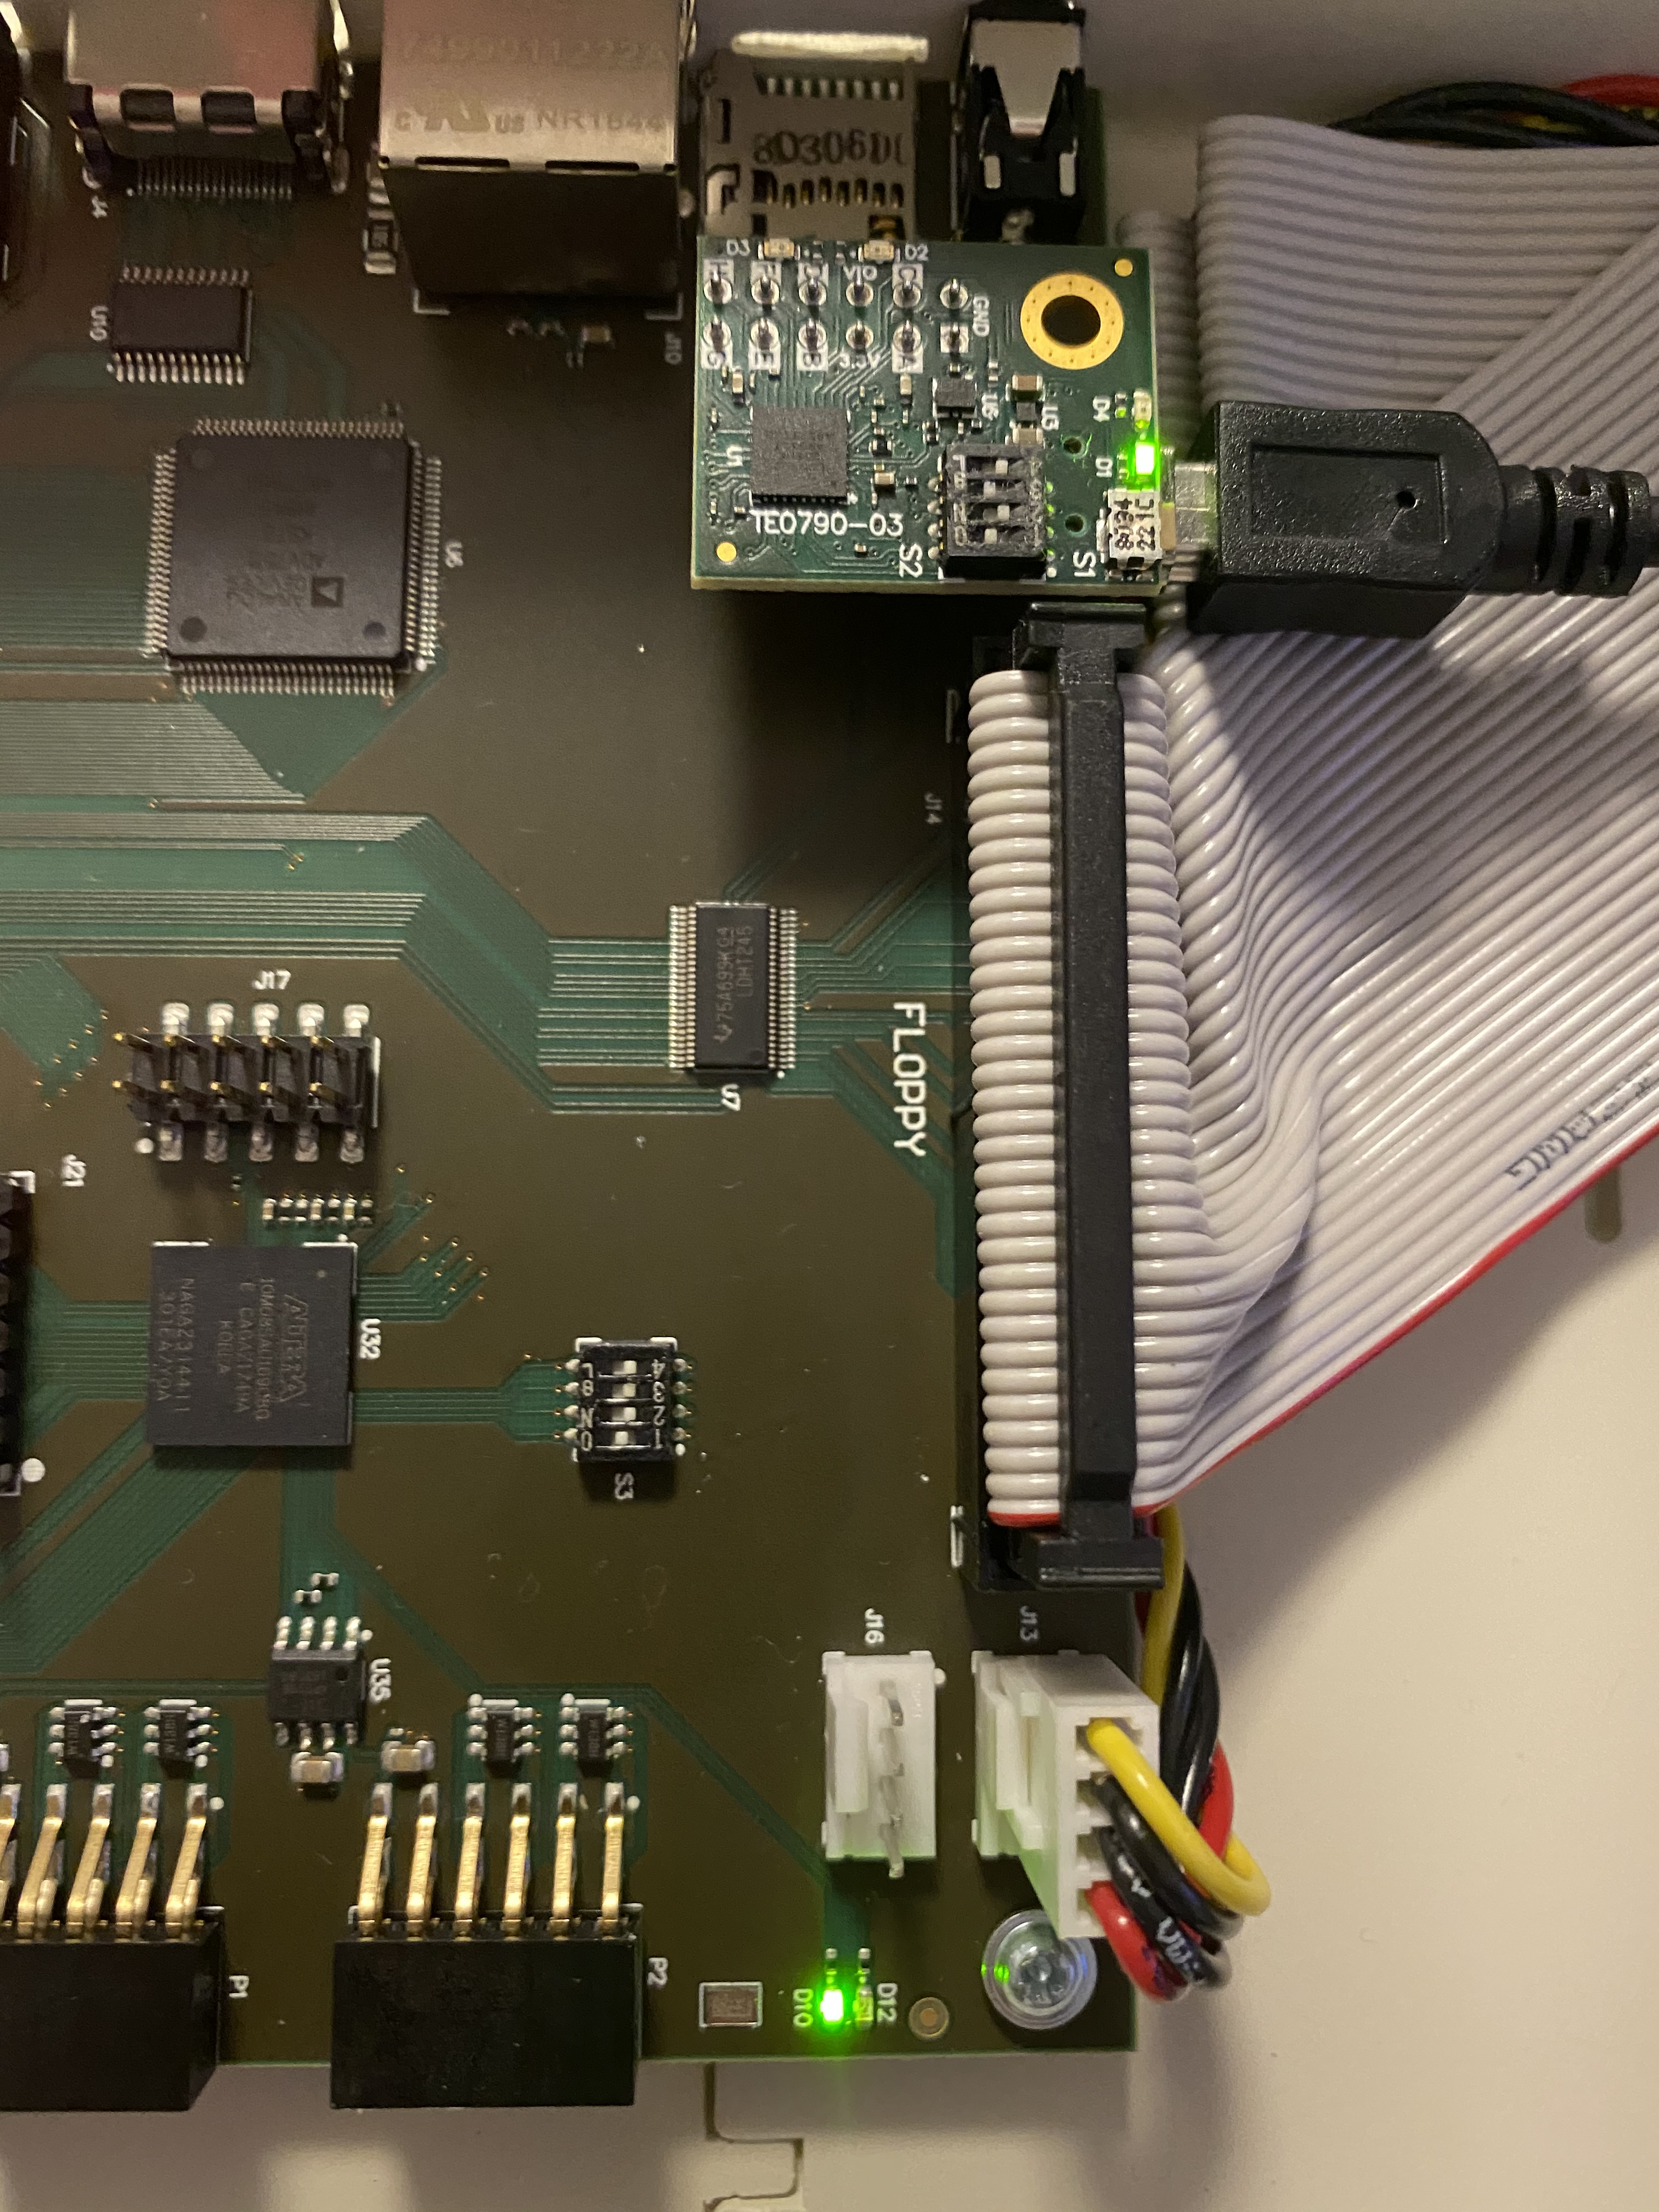
\includegraphics[width=\linewidth]{images/jtag_detail_05.jpg}

Connect your non-8-bit computer to the FPGA programming device using a micro-USB cable.
Open Quartus Prime Programmer Lite Edition, which can be downloaded from the internets.

\begin{figure}
  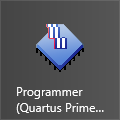
\includegraphics{images/max10_01.png}
  \caption{Step 1: Open Quartus Prime Programmer Lite Edition}
  \label{fig:max10_01}
\end{figure}

Click the "Hardware Setup" button in the top left corner of the Quartus Prime Programmer window.

\begin{figure}
  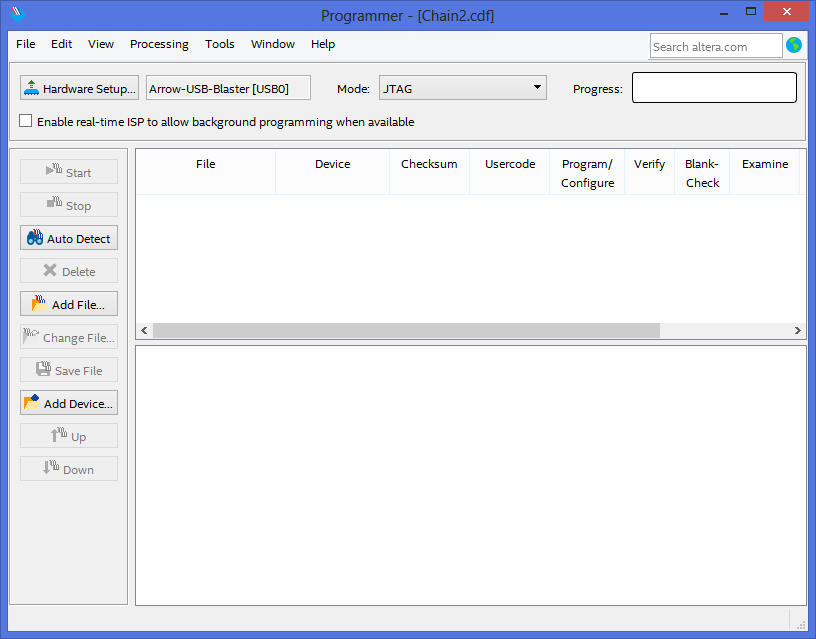
\includegraphics[width=\linewidth]{images/max10_02.png}
  \caption{Step 2: Enter Hardware Setup}
  \label{fig:max10_02}
\end{figure}

In the newly appeared window under "Currently selected hardware" choose "Arrow-USB-Blaster".
If "Arrow-USB-Blaster" does not appear, verify cable and drivers being correctly installed.

\begin{figure}
  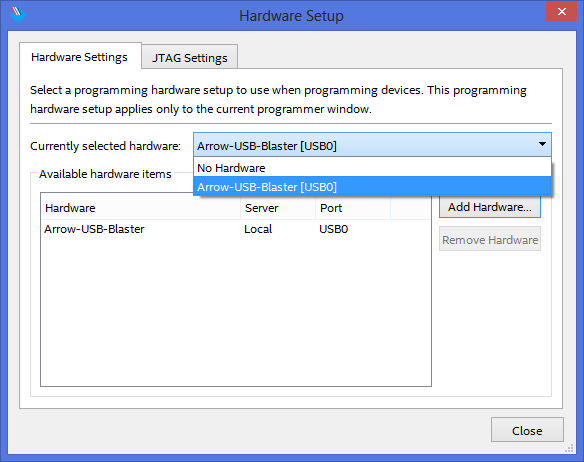
\includegraphics[width=\linewidth]{images/max10_03.png}
  \caption{Step 3: Select Arrow USB-Blaster}
  \label{fig:max10_03}
\end{figure}

Click the "Add File" button from the left row and choose the latest ".pof" file. Then click "Open".

\begin{figure}
  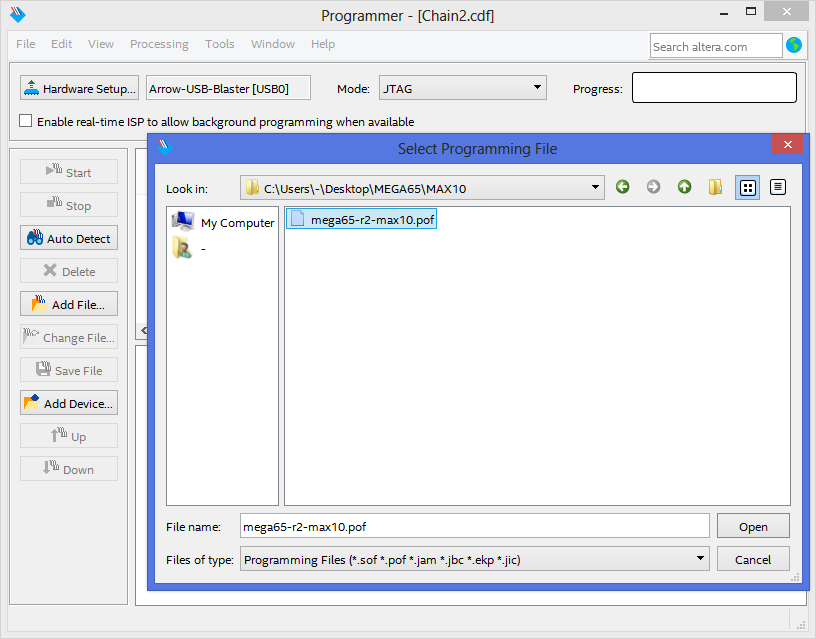
\includegraphics[width=\linewidth]{images/max10_04.png}
  \caption{Step 4: Select Programming File}
  \label{fig:max10_04}
\end{figure}

Tick at least the three boxes under "Program/Configure". Also enabling all boxes under "Verify" and "Blank-Check"
will make the process more reliable.

\begin{figure}
  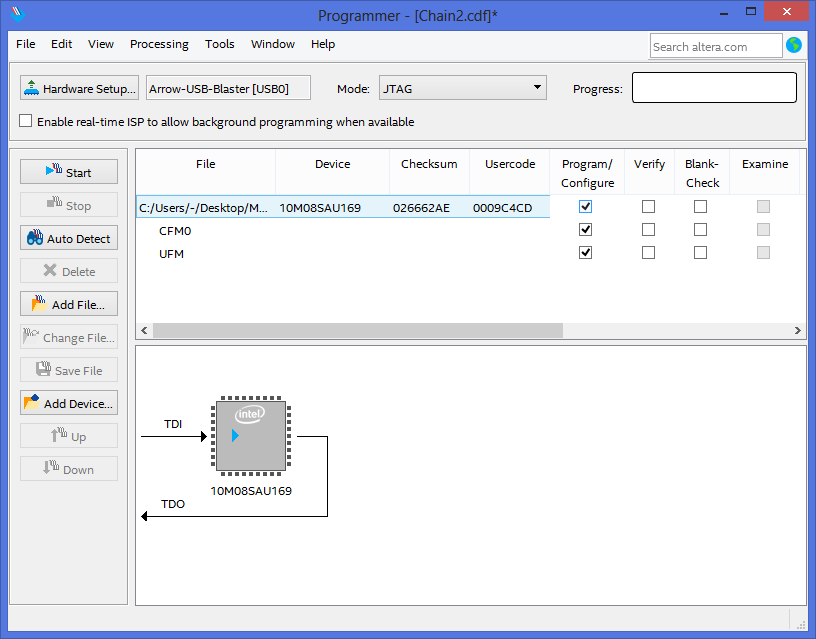
\includegraphics[width=\linewidth]{images/max10_05.png}
  \caption{Step 5: Select Program/Configure Options}
  \label{fig:max10_05}
\end{figure}

While keeping the Reset-Button pressed, switch the MEGA65 computer ON. The keyboard will go into "Police Mode"
(blue and red blinking LEDs). If it does not, the ARTIX 100T is not empty - restart the whole process.

Now click on "Start" in the left row of buttons. The progress bar in the top right corner should quickly go to
100 percent and turn green. You have now successfully updated your MAX10 FPGA!

If you receive an error message instead, make sure the ARTIX 100T bitstream has been erased and you did not
release the reset-button on the MEGA65 before - switch off the MEGA65 and restart this step.

\begin{figure}
  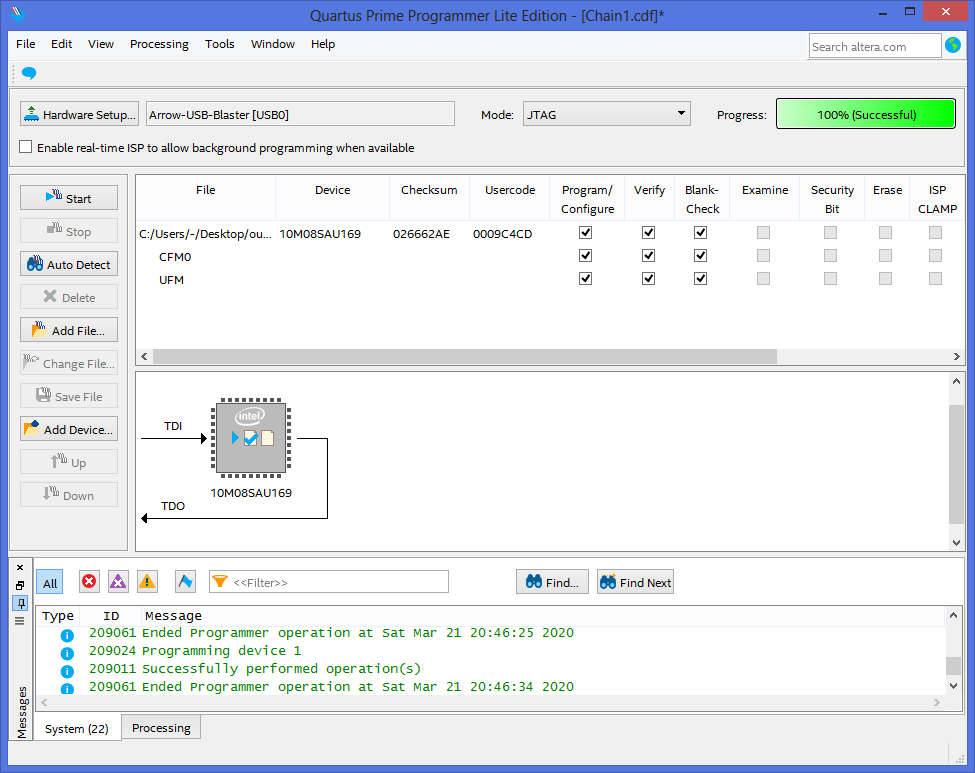
\includegraphics[width=\linewidth]{images/max10_06.png}
  \caption{Step 6: Programming successful}
  \label{fig:max10_06}
\end{figure}

  \chapter{Supporters \& Donors}

The MEGA65 would not have been possible to create without the generous support
of many organisations and individuals.

We are still compiling these lists, so apologies if we haven't included you yet.  If you
know anyone we have left out, please let us know, so that we can recognise the contribution
of everyone who has made the MEGA65 possible, and into the great retro-computing project
that it has become.

\section{Organisations}

\begin{itemize}
\item {\bf The MEGA Museum of Electronic Games \& Art e.V. Germany} \megakey{Everything}
\item {\bf Trenz Electronik, Germany} \megakey{Motherboard}
\item {\bf Hintsteiner, Austria} \megakey{Case}
\item {\bf GMK, Germany} \megakey{Keyboard}
\end{itemize}

\section{Contributors}

\setlength{\tabcolsep}{1mm}
\begin{tabular}{p{6cm}p{6cm}}

{\large\bf Andreas Liebeskind}     & {\large\bf Dr. Canan Hastik} \\
 \textit{(libi in paradize)}       & \textit{(indica)} \\
CFO MEGA eV                        & Chairwoman MEGA eV \\
& \\
{\large\bf Gurce Isikyildiz}       & {\large\bf Simon Jameson} \\
 \textit{(Gurce)}                  &  \textit{(Shallan)} \\
Tools and enhancements             & Platform Enhancements \\
& \\
{\large\bf Russell Peake}          & {\large\bf Stephan Kleinert} \\
  \textit{(rdpeake)}               & \textit{(ubik)}        \\
Bug Herding                        & Destroyer of BASIC 10     \\
& \\
{\large\bf Alexander Nik Petra}    & {\large\bf Wayne Johnson} \\
 \textit{(n0d)}                    &  \textit{(sausage)} \\
Early Case Design                  & Manual Additions \\
& \\
{\large\bf Ralph Egas}             & {\large\bf Lukas Kleiss} \\
 \textit{(0-limits)}               & \textit{(LAK132)} \\
Business Advisor                   & MegaWAT Presentation Software \\
& \\
{\large\bf Lucas Moss}             & {\large\bf Maurice van Gils }  \\
                                   & \textit{(Maurice)}  \\
MEGAphone PCB Design               & BASIC-65 example programs \\
& \\
{\large\bf Daren Klamer}           \\
 \textit{(Impakt)}                 \\
Manual proof-reading               \\
& \\
\end{tabular}

\newpage
\section{Supporters}

% page 1
\setlength{\tabcolsep}{1mm}
\begin{tabular}{p{4.5cm}p{4.5cm}p{4.5cm}}
@11110110100 & Arne Neumann & Christian Gräfe \\
3c74ce64 & Arne Richard Tyarks & Christian Heffner \\
8-Bit Classics & Axel Klahr & Christian Kersting \\
Aaron Smith & Balaz Ondrej & Christian Streck \\
Achim Mrotzek & Barry Thompson & Christian Wyk \\
Adolf Nefischer & Benjamin Maas & Christoph Haug \\
Adrian Esdaile & Bernard Alaiz & Christoph Huck \\
Adrien Guichard & Bernhard Zorn & Christoph Pross \\
Ahmed Kablaoui & Bieno Marti-Braitmaier & Christopher Christopher \\
Alan Bastian Witkowski & Bigby & Christopher Kalk \\
Alan Field & Bill LaGrue & Christopher Kohlert \\
Alberto Mercuri & Bjoerg Stojalowski & Christopher Nelson \\
Alexander Haering & Björn Johannesson & Christopher Taylor \\
Alexander Kaufmann & Bjørn Melbøe & Christopher Whillock \\
Alexander Niedermeier & Bo Goeran Kvamme & Claudio Piccinini \\
Alexander Soppart & Boerge Noest & Claus Skrepek \\
Alfonso Ardire & Bolko Beutner & Collen Blijenberg \\
Amiga On The Lake & Brett Hallen & Constantine Lignos \\
Andre Kapp & Brian Gajewski & Crnjaninja \\
André Kudra & Brian Green & Daniel Auger \\
André Simeit & Brian Juul Nielsen & Daniel Julien \\
André Wösten & Brian Reiter & Daniel Lobitz \\
Andrea Farolfi & Bryan Pope & Daniel O'Connor \\
Andrea Minutello & Burkhard Franke & Daniel Teicher \\
Andreas Behr & Byron Goodman & Daniel Tootill \\
Andreas Freier & Cameron Roberton (KONG) & Daniel Wedin \\
Andreas Grabski & Carl Angervall & Daniele Benetti \\
Andreas Millinger & Carl Danowski & Daniele Gaetano Capursi \\
Andreas Nopper & Carl Stock & Dariusz Szczesniak \\
Andreas Wendel Manufaktur & Carl Wall & Darrell Westbury \\
Andreas Zschunke & Carlo Pastore & David Asenjo Raposo \\
Andrew Bingham & Carlos Silva & David Dillard \\
Andrew Dixon & Carsten Sørensen & David Gorgon \\
Andrew Mondt & Cenk Miroglu Miroglu & David Norwood \\
Andrzej Hłuchyj & Chang sik Park & David Raulo \\
Andrzej Sawiniec & Charles A. Hutchins Jr. & David Ross \\
Andrzej Śliwa & Chris Guthrey & de voughn accooe \\
Anthony W. Leal & Chris Hooper & Dean Scully \\
Arkadiusz Bronowicki & Chris Stringer & Dennis Jeschke \\
Arkadiusz Kwasny & Christian Boettcher & Dennis Schaffers \\
Arnaud Léandre & Christian Eick & Dennis Schierholz \\
Arne Drews & Christian Gleinser & Dennis Schneck \\
\end{tabular}
% page 2
\newpage
\setlength{\tabcolsep}{1mm}
\begin{tabular}{p{4.5cm}p{4.5cm}p{4.5cm}}
denti & Frank Hempel & Henning Harperath \\
Dick van Ginkel & Frank Koschel & Henri Parfait \\
Diego Barzon & Frank Linhares & Henrik Kühn \\
Dierk Schneider & Frank Wolf & Holger Burmester \\
Dietmar Krueger & FranticFreddie & Holger Sturk \\
Dietmar Schinnerl & Fredrik Ramsberg & Howard Knibbs \\
Dirk Becker & Fridun Nazaradeh & Hubert de Hollain \\
Dirk Wouters & Friedel Kropp & Huberto Kusters \\
Domingo Fivoli & Garrick West & Hugo Maria Gerardus v.d. Aa \\
DonChaos & Gary Lake-Schaal & Humberto Castaneda \\
Donn Lasher & Gary Pearson & Ian Cross \\
Douglas Johnson & Gavin Jones & IDE64 Staff \\
Dr. Leopold Winter & Geir Sigmund Straume & Igor Ianov \\
Dusan Sobotka & Gerd Mitlaender & Immo Beutler \\
Earl Woodman & Giampietro Albiero & Ingo Keck \\
Ed Reilly & Giancarlo Valente & Insanely Interested Publishing \\
Edoardo Auteri & Gianluca Girelli & IT-Dienstleistungen Obsieger \\
Eduardo Gallardo & Giovanni Medina & Ivan Elwood \\
Eduardo Luis Arana & Glen Fraser & Jaap HUIJSMAN \\
Eirik Juliussen Olsen & Glen R Perye III & Jace Courville \\
Emilio Monelli & Glenn Main & Jack Wattenhofer \\
EP Technical Services & Gordon Rimac & Jakob Schönpflug \\
Epic Sound & GRANT BYERS & Jakub Tyszko \\
Erasmus Kuhlmann & Grant Louth & James Hart \\
ergoGnomik & Gregor Bubek & James McClanahan \\
Eric Hildebrandt & Gregor Gramlich & James Sutcliffe \\
Eric Hill & Guido Ling & Jan Bitruff \\
Eric Jutrzenka & Guido von Gösseln & Jan Hildebrandt \\
Erwin Reichel & Guillaume Serge & Jan Iemhoff \\
Espen Skog & Gunnar Hemmerling & Jan Kösters \\
Evangelos Mpouras & Günter Hummel & Jan Peter Borsje \\
Ewan Curtis & Guy Simmons & Jan Schulze \\
Fabio Zanicotti & Guybrush Threepwood & Jan Stoltenberg-Lerche \\
Fabrizio Di Dio & Hakan Blomqvist & Janne Tompuri \\
Fabrizio Lodi & Hans Pronk & Jannis Schulte \\
FARA Gießen GmbH & Hans-Jörg Nett & Jari Loukasmäki \\
FeralChild & Hans-Martin Zedlitz & Jarrod Adams \\
First Choice Auto's & Harald Dosch & Jason Smith \\
Florian Rienhardt & Harri Salokorpi & Javier Gonzalez Gonzalez \\
Forum64. de & Harry Culpan & Jean-Paul Lauque \\
Francesco Baldassarri & Heath Gallimore & Jeffrey van der Schilden \\
Frank Fechner & Heinz Roesner & Jens Schneider \\
Frank Glaush & Heinz Stampfli & Jens-Uwe Wessling \\
Frank Gulasch & Helge Förster & Jesse DiSimone \\
Frank Haaland & Hendrik Fensch & Johan Arneklev \\
\end{tabular}
% page 3
\newpage
\setlength{\tabcolsep}{1mm}
\begin{tabular}{p{4.5cm}p{4.5cm}p{4.5cm}}
Johan Svensson & Kosmas Einbrodt & Marcus Linkert \\
Johannes Fitz & Kurt Klemm & Marek Pernicky \\
John Cook & Lachlan Glaskin & Mario Esposito \\
John Deane & Large bits collider & Mario Fetka \\
John Nagi & Lars Becker & Mario Teschke \\
John Rorland & Lars Berntsson & Mariusz Tymków \\
John Sargeant & Lars Edelmann & Mark Adams \\
John Traeholt & Lars Slivsgaard & Mark Green \\
Jon Sandelin & Lasse Lambrecht & Mark Hucker \\
Jonas Bernemann & Lau Olivier & Mark Leitiger \\
Jonathan Prosise & Lee Chatt & Mark Spezzano \\
Joost Honig & Loan Leray & Mark Watkin \\
Jordi Pakey-Rodriguez & Lorenzo Quadri & Marko Rizvic \\
Jöre Weber & Lorenzo Travagli & Markus Bieler \\
Jörg Jungermann & Lorin Millsap & Markus Bonet \\
Jörg Schaeffer & Lothar James Foss & Markus Dauberschmidt \\
Jörg Weese & Lothar Serra Mari & Markus Fehr \\
Josef Hesse & Luca Papinutti & Markus Fuchs \\
Josef Soucek & Ludek Smetana & Markus Guenther-Hirn \\
Josef Stohwasser & Lukas Burger & Markus Liukka \\
Joseph Gerth & Lutz-Peter Buchholz & Markus Merz \\
Jovan Crnjanin & Luuk Spaetgens & Markus Roesgen \\
Juan Pablo Schisano & Mad Web Skills & Markus Uttenweiler \\
Juan S. Cardona Iguina & MaDCz & Martin Bauhuber \\
JudgeBeeb & Magnus Wiklander & Martin Benke \\
Juliussen Olsen & Maik Diekmann & Martin Gendera \\
Juna Luis Fernandez Garcia & Malte Mundt & Martin Groß \\
Jürgen Endras & Manfred Wittemann & Martin Gutenbrunner \\
Jürgen Herm Stapelberg & Manuel Beckmann & Martin Johansen \\
Jyrki Laurila & Manzano Mérida & Martin Marbach \\
Kai Pernau & Marc "3D-vice" Schmitt & Martin Sonnleitner \\
Kalle Pöyhönen & Marc Bartel & Martin Steffen \\
Karl Lamford & Marc Jensen & Marvin Hardy \\
Karl-Heinz Blum & Marc Schmidt & Massimo Villani \\
Karsten Engstler & Marc Theunissen & Mathias Dellacherie \\
Karsten Westebbe & Marc Tutor & Mathieu Chouinard \\
Keith McComb & Marc Wink & Matthew Adams \\
Kenneth Dyke & Marcel Buchtmann & Matthew Browne \\
Kenneth Joensson & Marcel Kante & Matthew Carnevale \\
Kevin Edwards & Marco Beckers & Matthew Palmer \\
Kevin Thomasson & Marco Cappellari & Matthew Santos \\
Kim Jorgensen & Marco Rivela & Matthias Barthel \\
Kim Rene Jensen & Marco van de Water & Matthias Dolenc \\
Kimmo Hamalainen & Marcus Gerards & Matthias Fischer \\
Konrad Buryło & Marcus Herbert & Matthias Frey \\
\end{tabular}
% page 4
\newpage
\setlength{\tabcolsep}{1mm}
\begin{tabular}{p{4.5cm}p{4.5cm}p{4.5cm}}
Matthias Grandis & Mikko Hämäläinen & Pauline Brasch \\
Matthias Guth & Mikko Suontausta & Paulo Apolonia \\
Matthias Lampe & Mirko Roller & Pete Collin \\
Matthias Meier & Miroslav Karkus & Pete of Retrohax.net \\
Matthias Mueller & Morgan Antonsson & Peter Eliades \\
Matthias Nofer & Moritz & Peter Gries \\
Matthias Schonder & Morten Nielsen & Peter Habura \\
Max Ihlenfeldt & MUBIQUO APPS,SL & Peter Herklotz \\
Meeso Kim & Myles Cameron-Smith & Peter Huyoff \\
Michael Dailly & Neil Moore & Peter Leswell \\
Michael Dötsch & Nelson & Peter Weile \\
Michael Dreßel & neoman & Petri Alvinen \\
Michael Fichtner & Nicholas Melnick & Philip Marien \\
Michael Fong & Nikolaj Brinch Jørgensen & Philip Timmermann \\
Michael Geoffrey Stone & Nils Andreas & Philipp Rudin \\
Michael Gertner & Nils Eilers & Pierre Kressmann \\
Michael Grün & Nils Hammerich & Pieter Labie \\
Michael Habel & Nils77 & Piotr Kmiecik \\
Michael Härtig & Norah Smith & Power-on.at \\
Michael Haynes & Norman King & Przemysław Safonow \\
Michael J Burkett & Normen Zoch & Que Labs \\
Michael Jensen & Olaf Grunert & R Welbourn \\
Michael Jurisch & Ole Eitels & R-Flux \\
Michael Kappelgaard & Oliver Boerner & Rafał Michno \\
Michael Kleinschmidt & Oliver Brüggmann & Rainer Kappler \\
Michael Lorenz & Oliver Graf & Rainer Weninger \\
Michael Mayerhofer & Oliver Smith & Ralf Griewel \\
Michael Nurney & Olivier Bori & Ralf Reinhardt \\
Michael Rasmussen & ONEPSI LLC & Ralf Schenden \\
Michael Richmond & oRdYNe & Ralf Smolarek \\
Michael Sachse & Osaühing Trioflex & Ralf Zenker \\
Michael Sarbak & OSHA-PROS USA & Ralph Bauer \\
Michael Scholz & Padawer & Ralph Wernecke \\
Michael Timm & Patrick Becher & Rédl Károly \\
Michael Traynor & Patrick Bürckstümmer & Reiner Lanowski \\
Michael Whipp & Patrick de Zoete & Remi Veilleux \\
Michal Ursiny & Patrick Toal & Riccardo Bianchi \\
Michele Chiti & Patrick Vogt & Richard Englert \\
Michele Perini & Paul Alexander Warren & Richard Good \\
Michele Porcu & Paul Gerhardt (KONG) & Richard Menedetter \\
Miguel Angel Rodriguez Jodar & Paul Jackson & Richard Sopuch \\
Mikael Lund & Paul Johnson & Rick Reynolds \\
Mike Betz & Paul Massay & Rico Gruninger \\
Mike Kastrantas & Paul Westlake & Rob Dean \\
Mike Pikowski & Paul Woegerer & Robert Bernardo \\
\end{tabular}
% page 5
\newpage
\setlength{\tabcolsep}{1mm}
\begin{tabular}{p{4.5cm}p{4.5cm}p{4.5cm}}
Robert Eaglestone & Stefan Haberl & Thomas Schilling \\
Robert Grasböck & Stefan Kramperth & Thomas Tahsin-Bey \\
Robert Miles & Stefan Richter & Thomas Walter \\
Robert Schwan & Stefan Schultze & Thomas Wirtzmann \\
Robert Shively & Stefan Sonnek & Thorsten Knoll \\
Robert Tangmar & Stefan Theil & Thorsten Nolte \\
Robert Trangmar & Stefan Vrampe & Tim Krome \\
Rodney Xerri & Stefano Canali & Tim Waite \\
Roger Olsen & Stefano Mozzi & Timo Weirich \\
Roger Pugh & Steffen Reiersen & Timothy Blanks \\
Roland Attila Kett & Stephan Bielmann & Timothy Henson \\
Roland Evers & Stephen Jones & Timothy Prater \\
Roland Schatz & Steve Gray & Tobias Butter \\
Rolf Hass & Steve Kurlin & Tobias Heim \\
Ronald Cooper & Steve Lemieux & Tobias Köck \\
Ronald Hunn & Steven Combs & Tobias Lüthi \\
Ronny Hamida & Stewart Dunn & Tommi Vasarainen \\
Ronny Preiß & Stuart Marsh & Toni Ammer \\
Roy van Zundert & Sven Neumann & Tore Olsen \\
Rüdiger Wohlfromm & Sven Stache & Torleif Strand \\
Ruediger Schlenter & Sven Sternberger & Torsten Schröder \\
Rutger WIllemsen & Sven Wiegand & Tuan Nguyen \\
Sampo Peltonen & Szabolcs Bence & Uffe Jakobsen \\
Sarmad Gilani & Tantrumedia Limited & Ulrich Hintermeier \\
SAS74 & Techvana Operations Ltd. & Ulrich Nieland \\
Scott Halman & Teddy Turmeaux & Ulrik Kruse \\
Scott Hollier & Teemu Korvenpää & Ursula Förstle \\
Scott Robison & The Games Foundation & Uwe Boschanski \\
Sebastian Baranski & Thierry Supplisson & Vedran Vrbanc \\
Sebastian Bölling & Thieu-Duy Thai & Verm Project \\
Sebastian Felzmann & Thomas Bierschenk & Wayne Sander \\
Sebastian Lipp & Thomas Edmister & Wayne Steele \\
Sebastian Rakel & Thomas Frauenknecht & Who Knows \\
Şemseddin Moldibi & Thomas Gitzen & Winfried Falkenhahn \\
Seth Morabito & Thomas Gruber & Wolfgang Becker \\
Shawn McKee & Thomas Haidler & Wolfgang Stabla \\
Siegfried Hartmann & Thomas Jager & Worblehat \\
Sigurbjorn Larusson & Thomas Karlsen & www.patop69.net \\
Sigurdur Finnsson & Thomas Laskowski & Yan B \\
Simon Lawrence & Thomas Marschall & Zoltan Markus \\
Simon Wolf & Thomas Niemann & Zytex Online Store \\
spreen.digital & Thomas Scheelen &  \\
\end{tabular}

\end{appendices}


\nocite{*}
\bibliographystyle{IEEEtran}
\bibliography{references}

\printindex


\end{document}


